\documentclass[twoside]{report}
\pagestyle{headings}
\usepackage[swedish]{babel}
\usepackage[utf8]{inputenc}
\usepackage{amsmath}
\usepackage{amssymb}
\usepackage{amsthm}
\usepackage{graphicx}
\usepackage{maplestd2e}


\newtheorem{Definition}{Definition}[chapter]
\newtheorem{Theorem}{Sats}[chapter]
\newtheorem{Lemma}{Lemma}[chapter]
\newtheorem{Corollary}{Följdsats}[chapter]


% Title Page
\title{Algoritmer inom \\
	kommutativ algebra \& algebraisk geometri \\[20pt]
	\large Omparametrisering av kurvor, semigrupper, \\
	implicit notation \& multiplicitetsföljder\\[15pt]
	\hrule \\[15pt]
	\Large Algorithms in\\
	commutative algebra \& algebraic geometry \\[20pt]
	\large Reparametrization of curves, semi-groups, \\
	implicit notation \& multiplicity sequences\\[20pt]}
\author{Peter Waher}


\begin{document}
\maketitle

\begin{abstract}
I denna rapport presenteras olika algoritmer inom ramen för kommutativ algebra och algebraisk geometri, med fokus på omparametrisering av algebraiska plana kurvor, semigrupper, implicit notation och multiplicitetsföljder. Höjdpunkter inkluderar egenutvecklade algoritmer för omparametriserar plana algebraiska kurvor på formen $(\pm t^n, p(t))$ eller $(p(t), \pm t^n)$, där $\mathbf{o}(p)\geq n$, beräkning av generatorerna till semigrupper motsvarande givna delringar i $\mathbb{C}[x_1,\ldots,x_n]$, sökning efter den implicita notationen för en kurva givet en parametrisering, generering av multiplicitetsföljder från den implicita notationen samt omvänt hitta funktionsfamiljer motsvarande en given multiplicitetsföljd. Rapporten avslutas med en empirisk studie i komplexiteten hos talföljden $N_i$ av antalet multiplicitetsföljder vars multiplicitetssumma motsvarar $i$.

\begin{center}
	\textbf{Abstract}
\end{center}

In this report various algorithms within the realm of commutative algebra and algebraic geometry are presented. The focus is set on re-parametrization of plane algebraic curves, semi-groups, implicit notation and multiplicity sequences. Highlights include self-developed algorithms that re-parametrize plane algebraic curves to the form $(\pm t^n, p(t))$ or $(p(t), \pm t^n)$, were $\mathbf{o}(p)\geq n$, calculation of the generators of semi-groups corresponding to given sub-rings to $\mathbb{C}[x_1,\ldots,x_n]$, search for the implicit notation of a curve, given a parametrization, generation of multiplicity sequences from the implicit notation as well as reversely find a family of curves that correspond to a given multiplicity sequence. The report finishes with an empiric study of the complexity of the number sequence $N_i$ of the number of multiplicity sequences whose multiplicity sum corresponds to $i$.
\end{abstract}

\section*{Förord}

Denna rapport, vilken är resultatet av ett självständigt arbete inom Matematik om 30 poäng, är en rapport av typ $\mathfrak{L}_2$, eller $\text{\emph{Lasaros}}^2$. Efter att ha avbrutit mina matematikstudier 1993 utan att ta examen för att arbeta med utveckling av TV-spel, gav professor Ralf Fröberg på matematiska institutionen vid Stockholms Universitet mig möjligheten att ta examen i matematik igen år 2002 då lusten att avsluta studierna gjorde sig känd. Efter att ha gjort klart största delen av arbetet, ville dock ödet sätta käppar i hjulet och ge mig en läxa, genom att få min dator och hårddisk att totalt haverera. Efter ett dyrbart besök hos en specialist på området gav jag dock upp hoppet om att kunna återskapa arbetet från de sektorer han lyckades rädda. \TeX är inte förlåtande, och tiden det skulle ta att återskapa arbetet från den genererade PDF-filen för att kunna skriva klart arbetet var för mycket för mig vid den tiden, då jag även jobbade samtidigt. Så jag avbröt mina studier, för andra gången, denna gång på grund av bristande tid och energi. Men, skam den som ger sig! År 2015 får jag åter igen möjlighet att göra klart arbetet, denna gång av Rikard Bögvad på samma universitet. Ralf Fröberg har nu blivit professor emeritus, men fortsätter som handledare. 


\tableofcontents{}

\chapter{Notation}

De symboler och notation som använts i detta dokument har kategoriserats och listats här nedan.

\section{Mängder}

\begin{tabular}{cp{10.5cm}}
$\varnothing$	& Den tomma mängden \\ 
$\in$	& \ldots är ett element i \ldots \\ 
$\notin$	&  \ldots är inte ett element i \ldots \\ 
$\cup$	& Unionen av två mängder \\ 
$\cap$	&  Skärningen av två mängder \\ 
$\setminus$	&  Komplementet av den högra mängden i den vänstra \\ 
$\subset$	& \ldots är en strikt delmängd av \ldots, dvs. de är inte lika \\ 
$\subseteq$	& \ldots är en delmängd av \ldots, och de kan vara lika \\ 
$\{ \ldots \}$	& Beskrivning av en mängd \\ 
$\left\|  \ldots \right\|$	& Antalet element i mängden \\ 
$\left\langle \ldots \right\rangle $	& Den mängd, semigrupp, grupp, ring, modul eller algebra som genereras av \ldots, beroende av kontexten. \\ 
\end{tabular} 

\section{Fördefinierade mängder}

\begin{tabular}{lp{10.5cm}}
$\mathbb{N}$ & De naturliga talen, inklusive noll: $0, 1, 2, 3, \ldots$ \\
$\mathbb{Z^+}$ & De positiva heltalen (exklusive noll): $1, 2, 3, \ldots$ \\
$\mathbb{Z}$ & Alla heltal \\
$\mathbb{R}$ & De reella talen \\
$\mathbb{C}$ & De komplexa talen
\end{tabular}

\section{Heltal}

\begin{tabular}{lp{10.5cm}}
$\mathbb{Z}_m$ & $\left\lbrace \left[ n \right] _m : n \in \mathbb{Z}\right\rbrace$ \,\, (skrivs även $\mathbb{Z}/\left\langle m \right\rangle$, $\mathbb{Z}/m$ eller $\mathbb{Z}/{m\mathbb{Z}}$) \\
$\left[ n \right] _m$ & $\left\lbrace a \in \mathbb{Z} : a \equiv n \pmod{m}\right\rbrace$ \\
$a \equiv n \pmod{m}$ & $\exists b \in \mathbb{Z} : a = n + b \cdot m$ \\
$a \mid b$ & $a$ delar $b$, dvs. $\exists n \in \mathbb{N} : b = a \cdot n$ \\
$a \nmid b$ & $a$ delar inte $b$
\end{tabular}

\section{Logiska operatorer}

\begin{tabular}{cp{10.5cm}}
$\exists$ & Existens av \ldots \\
$\forall$ & För alla \ldots \\
$\Longrightarrow$ & Logisk implikation \\
$\Longleftrightarrow$ & Logisk ekvivalens \\
$\vee$ & Logiskt eller \\
$\wedge$ & Logiskt och \\
$\neg$ & Logisk negation \\
$\therefore$ & Därför, logisk slutsats
\end{tabular}

\section{Relationer}

\begin{tabular}{cp{10.5cm}}
$\approx$ & $f \approx g$ betyder att $f$ är ungefär lika med $g$. Kan vara ett empiriskt antagande eller en förenkling.\\
$\sim$ & $f \sim g$ (då $n \rightarrow \infty$) betyder att $f$ är asymptotisk till $g$ (då $n$ går mot $\infty$), dvs. $\lim\limits_{n \rightarrow \infty}\frac{f(n)}{g(n)}=1$.\\
\end{tabular}
\section{Övrigt}

\begin{tabular}{cp{10.5cm}}
$0$ & Nollelementet i gruppen som behandlas. Kan även stå som förkortning
av $\left\lbrace 0\right\rbrace$. \\
$1$ & Ett elementet i ringen som behandlas. Kan även stå som förkortning
av $\left\lbrace 1\right\rbrace$. \\
$\mathbf{0}$ & $\left(0, \ldots , 0\right) \in \mathbb{C} ^n$ \\
$\infty$ & Oändligheten. Vilken oändlighet framgår av sammanhanget. \\
\end{tabular}

\chapter{Kurvor}
\label{Curves}

\section{Introduktion}

\begin{Definition}
En \textbf{plan kurva} $C$ är en delmängd i $\mathbb{C}^2$ sådan att det finns två kontinuerliga funktioner $f : \mathbb{R} \rightarrow \mathbb{C}$ och 
$g : \mathbb{R} \rightarrow \mathbb{C}$ sådana att $C = \left\{\left(f(t), g(t)\right) : t \in \mathbb{R}\right\}$. $(f, g)$ är en \textbf{parametrisering} av $C$. Om $C$ kan parametriseras av två analytiska funktioner $f$ och $g$ kallas $C$ \textbf{analytisk}. Om den kan parametriseras av två polynom kallas $C$ för \textbf{algebraisk}. Om den kan parametriseras av två formella potensserier kallas $C$ \textbf{algebroid}.
\end{Definition}

Eftersom vi kommer att studera kurvor lokalt, kommer de olika termerna nämnda ovan inte att skilja sig åt så mycket: Polynom är ju i sig formella potensserier där bara ett ändligt antal koefficienter är nollskilda. Analytiska funktioner kan också skrivas som formella potensserier som konvergerar i ett område kring den punkt vi vill studera.

För att förenkla notationen kan vi identifiera kurvan $C$ med en viss parametrisering $(f, g)$, även om parametriseringen inte är unik. Detta görs enklast genom att identifiera kurvan med funktionen $C : R \rightarrow \mathbb{C}^2$, $C(t) = \left(f(t), g(t)\right)$. Notera dock att kurvan som sådan och en av dess parametriseringar är två olika objekt.

När vi studerar egenskaper hos plana kurvor kan vi anta att kurvan går
genom origo, samt att $f(0) = g(0) = 0$, eller enklare skrivet $C(0) = \mathbf{0}$. Om så inte är fallet kan vi först göra en omparametrisering av $C$ och sedan ett enkelt byte av koordinatsystem:

Anta att $(f, g)$ är en parametrisering av $C$ och att vi vill studera kurvan
kring punkten $\left(x_0, y_0\right)$, och att $t = t_0$ är sådan att $x_0 = f(t_0)$ och $y_0 = g(t_0)$. Omparametriseringen kan vi göra på följande enkla sätt:

\begin{equation*}
\left\{
\begin{array}{lll}
f^*(t) & = & f(t+t_0) \\
g^*(t) & = & g(t+t_0) \\
C^*(t) & = & (f^*(t),g^*(t)) \\
\end{array}
\right.
\end{equation*}

Detta ger att $C^*(\mathbb{R}) = C(\mathbb{R})$, och kurvorna $C^*$ och $C$ är identiska. Koordinatbytet gör man enklast:

\begin{equation*}
\left\{
\begin{array}{lll}
x^{**} & = & x-x_0 \\
y^{**} & = & y-y_0 \\
f^{**}(t) & = & f^*(t)-x_0 \\
g^{**}(t) & = & g^*(t)-y_0 \\
C^{**}(t) & = & (f^{**}(t),g^{**}(t)) \\
\end{array}
\right.
\end{equation*}

Detta ger $C^{**}(\mathbb{R}) = C^*(\mathbb{R}) - (x_0, y_0) = C(\mathbb{R}) - (x_0, y_0)$ och $C^{**}(0) = \mathbf{0}$. I fortsättningen antar vi därför att de plana kurvor $C$ som vi studerar har egenskapen $C(0) = \mathbf{0}$.


\begin{Definition}
Om en kurva $C$ har en parametrisering $(f, g)$ sådan att $f'(0) \neq 0$ eller $g'(0) \neq 0$ kallas kurvan \textbf{reguljär}. Annars kallas kurvan \textbf{singulär}.
\end{Definition}

Bara för att $f'(0) = 0$ och $g'(0) = 0$ i en parametrisering $(f, g)$ av en
kurva $C$, betyder inte det att kurvan är singulär. Det kan ju finnas en parametrisering av samma kurva där någon av derivatorna är nollskilda. Exempelvis är $(t^3, t^3)$ och $(t, t)$ två olika parametriseringar av samma kurva. I det första exemplet är derivatorna $0$ i origo medan de i det andra
exemplet båda är nollskilda. (Notera dock att $(t^2, t^2)$ och $(t, t)$ inte motsvarar samma kurva. Den första innehåller inte punkterna $(t, t)$ för $t < 0$.)

\section{Omparametrisering av kurvor}

För att studera egenskaper hos en viss kurva $C = (f(t), g(t))$ kan det ibland vara intressant att göra en omparametrisering av kurvan till en enklare eller mer fördelaktig form. För utritande av kurvor spelar kanske parametriseringen inte så stor roll. Men vill man beräkna $y(x) = g(f^{-1}(x))$ eller $x(y) = f(g^{-1}(y))$ för motsvarande kurva, står man genast inför en mängd problem eftersom parametriseringen kan vara så generell. Ofta är det väldigt svårt att explicit hitta inversen av en analytisk funktion, även om den är så ``enkel'' som ett polynom. Dessutom brukar inverserna vara flervärda så man måste på något sätt bestämma sig för vilken del av kurvan man är intresserad av.

Vi kan väldigt lätt skapa omparametriseringar av kurvan $C$ ovan, genom
att ta en funktion $\phi(t)$ som är analytisk kring $t = 0$ och sådan att $\phi(0) = 0$, och därefter skapa parametriseringen \[C^*(t) = (f^*(t), g^*(t)) = (f(\phi(t)), g(\phi(t)))\]

Om $\phi(t)$, $f(t)$ och $g(t)$ är reellvärda är också parametriseringen $C^*(t)$ reellvärd.

Eftersom $\phi$ är analytisk kring $t = 0$ och $\phi(0) = 0$ vet vi att den är ett-till-ett i ett område kring $t = 0$. Detta säger oss att $\exists I1 \subseteq \mathbb{R}, I2 \subseteq \mathbb{R}$ sådana att $C^*(I1) = C(I2)$, dvs. kurvan som den nya parametriseringen $(f^*(t), g^*(t))$ bildar och den gamla $(f(t), g(t))$ överensstämmer ``delvis''. Är dessutom $\phi$ ett-till-ett i hela $\mathbb{R}$ gäller att $C^*(\mathbb{R}) = C(\mathbb{R})$ eller att kurvorna överensstämmer ``helt''.

Eftersom alla funktioner $\phi$ som är analytiska kring $t = 0$ och $\phi(0) = 0$ kan skrivas på formen \[\phi(t)=\sum_{k=1}^{\infty}a_k t^k\] i ett område kring $t = 0$ (även f(t) och g(t) kan ha denna form om $C$ är analytisk, algebraisk eller algebroid) skall vi studera våra möjligheter att skapa omparametriseringar av kurvan $C(t)$ med hjälp av potensserier.

Först några definitioner:

\begin{Definition}
\textbf{Ordningen} av ett polynom eller en potensserie $f(t) =
\sum a_i t^i \neq 0$ är det minsta heltalet $k$ sådant att koefficienten $a_k$ är nollskild, och skrivs $\mathbf{o}(f)$. \textbf{Graden} for motsvarande polynom är det största heltalet $k$ sådant att koefficienten $a_k$ inte är noll, och skrivs $\deg(f)$.
\end{Definition}

Om $\phi(t) = \sum a_k t^k$ och $f(t) = \sum b_k t^k$, hur ser då $f^*(t) = f(\phi(t)) = \sum c_k t^k$ ut? Följande vet vi: $\mathbf{o}(f^*) = \mathbf{o}(f(\phi)) = \mathbf{o}(f) \cdot \mathbf{o}(\phi)$, samt att \[c_{\mathbf{o}(f^*)}=b_{\mathbf{o}(f)} \cdot {a_{\mathbf{o}(\phi)}}^{\mathbf{o}(f)}\]

Om vi vill att $f^*(t)$ skall vara på formen $f^*(t) = t^n$, där $n = \mathbf{o}(f) \cdot \mathbf{o}(\phi)$, måste således \[a_{\mathbf{o}(\phi)} = \left(\frac{1}{b_{\mathbf{o}(f)}}\right)^\frac{1}{\mathbf{o}(f)} \neq 0\]

Betraktar man hela $\mathbb{C}$ finns $\mathbf{o}(f)$ olika lösningar för $a_{\mathbf{o}(\phi)}$. Dock skall vi försöka välja en lösning sådan att alla $a_k$ blir reella (förutsatt att alla $b_k$ är reella).

För att göra beräkningarna lite enklare och överskådligare, kan vi tills vidare begränsa oss till att bara betrakta funktioner $\phi(t)$ sådana att $a_1 \neq 0$, dvs. att $\mathbf{o}(\phi)=1$. Detta medför att $n = \mathbf{o}(f^*) = \mathbf{o}(f)$ och att 
\[c_n=b_n \cdot {a_1}^n\]

och vi får
\[a_1 = \left(\frac{1}{b_n}\right)^\frac{1}{n} \neq 0\]

vilket har $n$ lösningar i $\mathbb{C}$. Den andra koefficienten $c_{n+1}$ i $f^*$ får följande utseende:
\[c_{n+1} = b_{n+1} {a_1}^{n+1} + n b_n {a_1}^{n-1} a_2\]

Eftersom $n \neq 0$, $b_n \neq 0$ och $a_1 \neq 0$ är detta en linjär ekvation i $a_2$ med en unik lösning. Eftersom vi vill att $f^*$ skall vara på formen $f^*(t) = t^n$ sätter vi således $c_{n+1} = 0$, och vi får:

\[a_2 = -\frac{b_{n+1} {a_1}^{n+1}}{n b_n {a_1}^{n-1}}=-\frac{b_{n+1}}{n b_n} {a_1}^2\]

Vi antar nu att $a_1, \ldots, a_m$ är beräknade och att $c_{n+1} = \ldots = c_{n+m-1} = 0$. För att beräkna $a_{m+1}$ tittar vi på $c_{n+m}$, och sätter denna till $0$. $c_{n+m}$ har bidrag från de $m + 1$ lägsta potenserna i $f(\phi(t))$: $b_n\phi(t)^n$, $b_{n+1}\phi(t)^{n+1}$, \ldots, $b_{n+m}\phi(t)^{n+m}$.

Från $b_{n+m} \phi(t)^{n+m}$ fås ett bidrag $b_{n+m} {a_1}^{n+m}$, som är en konstant (vi har ju antagit att $a1,\ldots,a_m$ är givna). Alla andra termer i denna potens har en grad större än $m + n$.

Från $b_{n+m-k} \phi(t)^{n+m-k}$ skapas en mängd termer på formen
\[b_{n+m-k} \cdot \prod_{j=1}^{n+m-k} a_{i_j} t^{i_j} = b_{n+m-k} \cdot \left( \prod_{j=1}^{n+m-k} a_{i_j} \right) t^{\sum i_j} \]
för alla olika talserier $\{i_j\}_1^{n+m-k}$ där $i_j \in \mathbb{Z}^+$ (dvs. $i_j \geq 1$). (Två talserier $\{i_j\}$ och $\{i^*_j\}$ anses lika, om $i_j=i^*_j, \forall j$.) Till koefficienten $c_{n+m}$ bidrar bara termer sådana att $\sum i_j = n+m$. Eftersom $i_j \geq 1$ får vi att $\sum i_j \geq n+m-k$, oavsett val av $\{i_j\}$. $\sum i_j = n+m-k$ fås om $i_j = 1, \forall j$. Det högsta $a_i$ som kan förekomma i termen $c_{n+m}$, motsvarar det största värde $i_j$ kan anta, vilket fås om alla $\{i_j\}$ förutom ett (det största) är $1$:
\[\max \left( i_j \Bigm| \sum i_j = n+m \right) = (n+m)-(n+m-k-1)=k+1\] 
$a_{k+1}$ motsvarar således koefficienten i $\phi$ av högst ordning som förekommer i $c_{n+m}$. Vi ser ytterligare att termen där denna koefficient förekommer har formen:
\[b_{n+m-k} {a_1}^{n+m-k-1} a_{k+1} t^{n+m}\]
Nämnda val av $\{i_j\}$ kan endast göras på $n + m - k$ olika sätt.

Av ovanstående resonemang ser man att bidragen till $c_{n+m}$ från termerna $b_{n+m-k} \phi(t)^{n+m-k}$ är konstanta (bara beroende av $a_1, \ldots, a_m$), för $k = 0, \ldots , m - 1$, och att bidraget från $b_n \phi(t)^n$ (dvs. då $k = m$) till $c_{n+m}$ är på formen
\[A_m(a1, \ldots, a_m) + b_n n {a_1}^{n-1} a_{m+1}\]
där $A_m(a1, \ldots, a_m)$ är en konstant (bara beroende av de givna $a_1, \ldots, a_m$). Om vi kallar bidragen från $b_{n+m-k} \phi(t)^{n+m-k}$ till $c_{n+m}$ ($0 \leq k \leq m-1$) för $B_m(a1, \ldots, a_m)$, vilket vi också såg bara beror på $a_1, \ldots, a_m$, får vi alltså:
\[c_{n+m} = A_m(a_1, \ldots, a_m) + B_m(a_1, \ldots, a_m) + n b_n {a_1}^{n-1} a_{m+1}\]

Eftersom det var givet att $b_n \neq 0$, $n \neq 0$ och att $a_1 \neq 0$ ser vi att ekvationen $c_{n+m} = 0$ har en unik lösning:
\[a_{m+1} = -\frac{A_m(a_1, \ldots, a_m) + B_m(a_1, \ldots, a_m)}{n b_n {a_1}^{n-1}}\]
Värt att observera är följande: $A_m(a_1, \ldots, a_m)$ och $B_m(a_1, \ldots, a_m)$ beror bara på koefficienterna $a_1, \ldots, a_m$ och $\{b_j\}$. Om alla dessa koefficienter är reella är således också $a_{m+1}$ reell.

Vi är nu redo för följande sats.

\begin{Theorem}
\label{ReparametrizeTheorem}
Om $C = C(t) = \left(f(t), g(t)\right)$ är en analytisk, algebroid eller algebraisk kurva och $f(t)$ och $g(t)$ är reellvärda, samt att $f(0) = g(0) = 0$, kan kurvan $C$ omparametriseras på formen $C^*(t) = \left(\pm t^n, g^*(t)\right)$ eller på formen $C^*(t) = \left(f^*(t), \pm t^n \right)$ i ett intervall kring $t = 0$, där $f(t)$ och $g(t)$ är formella potensserier. Dessutom gäller att $\mathbf{o}\left(f^*\right) \geq n$ eller att $\mathbf{o}\left(g^*\right) \geq n$.
\end{Theorem}

\begin{proof}
Vi kan utan att begränsa oss anta att $f(t)$ och $g(t)$ kan skrivas som potensserier kring $t = 0$. Vi antar först att $n = \mathbf{o}(f) \leq \mathbf{o}(g)$.

Från resonemanget ovan ser vi att vi kan skapa en formell potensserie $\phi(t) = \sum a_k t^k$ sådan att $f^*(t) = f\left(\phi(t)\right) = b_n {a_1}^n t^n = c \cdot t^n$. Vi vill välja $a_1$ sådan att $c = \pm 1$.

Om $n$ är udda, eller om $b_n > 0$ låter vi $c = 1$ vilket ger oss att
\[a_1 = \left( \frac{1}{b_n} \right) ^ \frac{1}{n}\]

Vi väljer här huvudgrenen för funktionen $x^{1/n}$, vilket ger oss ett reellt tal $a_1$. Om nu $n$ är ett jämnt tal och $b_n < 0$, låter vi istället $c = -1$ vilket ger oss att
\[a_1 = \left( \frac{1}{-b_n} \right) ^ \frac{1}{n}\]

Även detta tal är ett reellt tal. Om $f(t)$ är reellvärd består dess potensserie bara av reellvärda koefficienter ($\{b_k\}$). Eftersom $a_1$ är reellvärd fås med induktion att alla $a_k$ också är reellvärda, för $k > 1$. Detta ger oss att $g^*(t) = g\left(\phi(t)\right)$ också är reellvärd. Dessutom fås att
\[\mathbf{o}(g^*) = \mathbf{o}(g) \cdot \mathbf{o}(\phi) = \mathbf{o}(g) \cdot 1 = \mathbf{o}(g) \geq \mathbf{o}(f)\]

Om nu istället $\mathbf{o}(f) > \mathbf{o}(g)$, väljer vi $\phi(t)$ sådan att $g^*(t) = g\left(\phi(t)\right) = \pm t^n$. Resten av beviset är identiskt med ovanstående diskussion, vilket avslutar beviset.
\end{proof}

Från \emph{Weierstrass Preparation Theorem} \cite{WeierstrassPreparationTheorem} får man att en sådan omparametrisering existerar. Dock presenteras inte en metod över hur en sådan omparametrisering kan tas fram. Genom ovanstående bevis ges inte bara existensen utan även en metod över hur man kan skapa en sådan omparametrisering, givet en algebraisk eller algebroid plan kurva. En analytisk plan kurva kan parametriseras i en delmängd av $\mathbb{R}$ med hjälp av potensserier, så en analytisk plan kurva kan ses som en delvis algebroid kurva kring varje punkt i $\mathbb{R}$.

I bilaga \ref{Reparametrize} på sidan \pageref{Reparametrize} finns även beskrivet en algoritm som beräknar ovanstående omparametrisering för en godtycklig algebraisk kurva, upp till en maximal grad.
\chapter{Semigrupper}

Vid studier av singulariteter hos algebraiska kurvor använder man ofta motsvarande semigrupp som invariant för klassificering. Innan vi fördjupar oss i just detta måste vi först lite i hast nämna några talteoretiska definitioner och satser, för att därefter fördjupa oss lite i semigrupper.

\section{Heltal modulo $p$}

\begin{Definition}
Heltalen $m \in \mathbb{Z}^+$ och $n \in \mathbb{Z}^+$ sägs vara \textbf{relativt prima} om $m \geq 2$, $n \geq 2$ samt $p \mid m \wedge p \mid n \Longrightarrow p = 1$.
\end{Definition}

Att $m$ och $n$ är relativt prima är identiskt med att säga att $\gcd(m, n) = 1$
(största gemensamma delaren).

\begin{Lemma}
\label{L1}
Om $m$ och $n$ är relativt prima och $0 < a < m$ gäller att $[a \cdot n]_m \neq 0$.
\end{Lemma}

\begin{proof}
Antag att $[a \cdot n]_m = 0$ och att $a > 0$:
\[\begin{array}{rcl}
[a \cdot n]_m = 0 & \Longrightarrow & \exists b \in \mathbb{Z}^+ : a \cdot n = b \cdot m \\
 & \Longrightarrow & m \mid a \qquad\text{(eftersom }\gcd(m, n) = 1\text{)} \\
 & \Longrightarrow & a \geq m
\end{array}\]
\end{proof}

\begin{Lemma}
\label{L2}
Om $m$ och $n$ är relativt prima och $0 < a, b < m$ gäller:
\[[a \cdot n]_m = [b \cdot n]_m \Longleftrightarrow a = b\]
\end{Lemma}

\begin{proof}
Vi kan utan att begränsa oss antaga att $a \geq b$:
\[\begin{array}{rcl}
[a \cdot n]_m = [b \cdot n]_m & \Longleftrightarrow & [(a - b) \cdot n]_m = 0 \\
 & \Longleftrightarrow & a - b = 0 \quad\text{(eftersom } 0 \leq a - b < m \text{ samt lemma \ref{L1})}
\end{array}\]
\end{proof}

\section{Semigrupper}

\begin{Definition}
För en \textbf{semigrupp} $G$, med den implicit definierade operatorn $+$ gäller:
\[0 \in G\]
\[a \in G \wedge b \in G \Longrightarrow (a + b) \in G\]
\end{Definition}

Notera skillnaden mellan en semigrupp och en grupp: Alla element i en grupp har även en additiv invers, dvs. i gruppen tillåts subtraktion. I en semigrupp är det tillräckligt med bara addition av element, samt att det finns ett noll-element.

\begin{Definition}
En serie tal $n_1, \ldots, n_k$ \textbf{genererar} semigruppen $G$ om
\[G = \left\{\sum_{i=1}^{k} a_i \cdot n_i : a_i \in \mathbb{N}\right\}\]
Detta skrivs även $G = \left<n_1, \ldots, n_k \right>$.
\end{Definition}

Notera att det är viktigt att särskilja mellan generation av semigrupper och grupper. Vid generering av grupper gäller det att $a_i \in \mathbb{Z}$. Det finns ingen annan skillnad i notationen. Notera också att med multiplikation med ett positivt heltal inom en semigrupp avses repetitiv användning av additionsoperatorn.

\begin{Theorem}
\label{S1}
Om $m$ och $n$ är relativt prima innehåller semigruppen $G = \left<m, n\right>$ alla tal större än eller lika med $c = (m - 1)(n - 1)$, men inte talet $c - 1$.
\end{Theorem}

\begin{proof}
Först betraktar vi hur $[n]_m$ genererar hela $\mathbb{Z}_m$. Från lemma \ref{L1} vet vi att:

\begin{equation*}
\begin{array}{rcc}
[n]_m & \neq & 0 \\
\left[2n\right]_m & \neq & 0 \\
\vdots \quad & \vdots & \vdots \\
\left[(m - 1) \cdot \, n\right]_m & \neq & 0 \\
\end{array}
\end{equation*}

Lemma \ref{L2} säger dessutom att dessa $m - 1$ värdena är unika. Vi har alltså
$m-1$ stycken unika nollskilda element i $\mathbb{Z}_m$, i vilket det bara finns $m-1$ nollskilda element. Tillsammans med $[0 \cdot n]_m=[0]_m=0$ genererar således serien hela $\mathbb{Z}_m$. Detta skrivs $\mathbb{Z}_m = \left< [n]_m \right>$.

I följande resonemang kan vi utan att begränsa oss anta att $m < n$. För att beräkna det högsta värdet som inte är med i $\left<m, n\right>$ använder vi oss av uteslutningsmetoden:

Först delar vi upp $\mathbb{N}$ i segment om $m$ element vardera:
\[\{0, \ldots, m - 1\}, \quad \{m, \ldots, 2m - 1\}, \quad \ldots\]

Därefter stryker vi helt enkelt tal efter tal ur $\left<m,n\right>$ tills det inte finns fler tal att stryka bort. Vi börjar med att stryka bort talet $0$, och alla dess motsvarigheter i $\mathbb{Z}_m$ ($m$, $2m$, \ldots). Därefter stryker vi $n$, och alla dess motsvarigheter i $\mathbb{Z}_m$ ($n + m$, $n + 2m$, \ldots), följt av $2n$ och dess motsvarigheter i $\mathbb{Z}_m$ ($2n + m$, $2n + 2m$, \ldots), ända tills vi strukit $(m-1)n$ och dess motsvarigheter i $\mathbb{Z}_m$: $(m - 1)n + m$, $(m - 1)n + 2m$, \ldots. Efter det är alla tal i $\left<m,n\right>$ strukna.

Värt att notera här är att inga av de tal som strukits under ovanstående process, stryks mer än en gång. För att se detta, antar vi att vi har två tal $a_1$ och $a_2$, sådana att $0 < a_1, a_2, < m$, och att $a_1 n + i_1 m = a_2 n + i_2 m$ för några $i_1, i_2 \in \mathbb{N}$. Detta ger oss i så fall att $(a_1-a_2)n = (i_2-i_1)m$. Eftersom $m$ och $n$ är relativt prima, måste $m \vert (a_1-a_2)$. Men detta är bara möjligt om $a_1-a_2=0$, dvs. $a_1=a_2$.

Vi vet också, att vi strukit alla tal större än eller lika med $(m-1)n$ ur $\mathbb{N}$. Skulle det finnas något tal $i$ större än  $(m-1)n$ i $\mathbb{N}$ som inte strukits, skulle alla tal som är på formen $i+j\cdot m$ inte heller vara strukna, enligt hur vi skapade tillvägagångssättet att stryka tal. Således skulle alla element i ekvivalensklassen $[i]_m$ inte heller vara strukna, och således skulle $[i]_m$ inte finnas med i $\left<[n]_m\right>$, då vi strukit alla tal i dess ekvivalensklasser. Men eftersom $\left<[n]_m\right>$ genererar hela $\mathbb{Z}_m$, leder detta till en motsägelse.

Vi vet nu att vi strukit alla tal från och med $(m-1)n$ ur $\mathbb{Z}$. Men det segment av $\mathbb{Z}$ som innehåller $(m-1)n$ innehåller inte några andra ostrukna tal, eftersom $m < n$. Det högsta ostrukna talet, och därför också det högsta tal som inte är element i $\left<m, n\right>$ är således $(m - 1)n - m$, dvs. motsvarigheten till $(m - 1)n$ i det segment som föregår segmentet där $(m - 1)n$ finns. Vi kan nu beräkna c:
\[c = (m - 1)n - m + 1 = mn - n - m + 1 = (m - 1)(n - 1)\]
\end{proof}

\section{Numeriska semigrupper}

\begin{Definition}
En \textbf{numerisk semigrupp} $G$ är en speciell form av semigrupp, där även följande villkor gäller:
\[
\begin{array}{rcl}
G & \subseteq & \mathbb{N} \\
\left\| \mathbb{N} \setminus G \right\| & < & \infty \\
\end{array}\]
\end{Definition}

\begin{Lemma}
$G = \left<m, n\right>$ i sats \ref{S1} är en numerisk semigrupp.
\end{Lemma}

\begin{proof}
\[\begin{array}{rcl}
0 & = & 0 \cdot m + 0 \cdot n \in G \\
a \in G \wedge b \in G & \Longleftrightarrow & \exists c, d, e, f \in \mathbb{N} : a = cm + dn \wedge b = em + fn \\
 & \Longrightarrow & a + b = (c + e)m + (d + f)n \in G \\
G & \subset & \mathbb{N} \quad\text{(per definition av } \left<m, n\right> \text{)} \\
\left\|\mathbb{N}\setminus G\right\| & \leq & c - 1 < \infty \\
\end{array}\]
\end{proof}

\begin{Definition}
I varje numerisk semigrupp $G$ finns det ett tal $c_G$ sådant att följande villkor uppfylls:
\[\begin{array}{rcl}
c_G & \in & G \\
n > c_G & \Longrightarrow & n \in G \\
c_G - 1 & \notin & G \\
\end{array}\]
$c_G$ kallas för \textbf{konduktören} för $G$. $c$ i sats \ref{S1} är konduktör för den numeriska semigruppen $G = \left<m, n\right>$.
\end{Definition}

\begin{Theorem}
\label{S2}
Om semigruppen $G = \left<n_1, \ldots, n_k\right>$ är numerisk så är den största gemensamma delaren av talen $\gcd(n_1, \ldots, n_k) = 1$.
\end{Theorem}

\begin{proof}
För varje $n \in G$ så $\exists a_i \in \mathbb{N} : n = \sum_{i=1}^{k} a_i n_i$. Eftersom $d \mid n_i, \forall i$ får vi att $d \mid n$ och att $\gcd(G) \geq d$. Men $d^* = gcd(G)$ kan inte vara större än $d$, eftersom detta skulle innebära att $d^* \mid n_i, \forall n$, vilket leder till en motsägelse. Således är $d^*=d$.
\[\therefore \gcd(G)=\gcd(n_1,\ldots,n_k)=d\] 

För att visa att $d=1$ om $G$ är numerisk, antar vi först motsatsen, dvs. att $d = \gcd(n_1, \ldots, n_k) \geq 2$:

\[\begin{array}{rcl}
d \geq 2 & \Longrightarrow & d \nmid a \cdot d + 1, a \in \mathbb{N} \\
 & \Longrightarrow & \left\{a \cdot d + 1 : a \in \mathbb{N}\right\} \cap G = \varnothing \\
 & \Longrightarrow & \left\{a \cdot d + 1 : a \in \mathbb{N}\right\} \subseteq \mathbb{N} \setminus G \\
 & \Longrightarrow & \left\|\mathbb{N} \setminus G \right\| = \infty \\
\end{array}\]
Således kan inte $G$ vara numerisk, vilket är en motsägelse.
\[\therefore \gcd(n_1, \ldots, n_k) = 1\]
\end{proof}

\begin{Theorem}
\label{S3}
Varje numerisk semigrupp $G$ har ett minimalt generatorsystem $n_1, \ldots, n_k$, dvs. $G = \left<n_1, \ldots, n_k\right>$. Detta system är unikt för $G$.
\end{Theorem}

\begin{proof}
Först skall vi bevisa att det finns en ändlig mängd tal i $G$ som genererar $G$. Eftersom $G$ är numerisk betyder detta att det finns ett största tal $N \in \mathbb{N} : (n > N \Longrightarrow n \in G)$. Välj $a$ och $b$ så att $2^a > N \wedge 3^b > N$. Detta ger att $2^a \in G \wedge 3^b \in G$. Men $\gcd(2^a, 3^b) = 1$ vilket enligt sats \ref{S1} ger oss att $\left<2^a, 3^b\right>$ innehåller alla tal större än eller lika med $c = (2^a - 1)(3^b - 1)$.
\[\therefore \left\{1, \ldots, c, 2^a, 3^b\right\} \cap G \text{ genererar } G\text{.}\]

Då vi vet att $G$ har ändliga generatorer kan vi skapa mängden $\widehat{M}$ som mängden av alla ändliga generatorer, och $\widehat{M}' = \{ \left\|M\right\| : M \in \widehat{M}\}$. Låt $k = \inf \widehat{M}'$. Eftersom $\widehat{M}'$ bara innehåller positiva heltal existerar $k$ samt $\exists M_- \in \widehat{M} : \left\|M_-\right\|=k$.

Antag nu att vi har ett annat generatorsystem $N_-$ sådant att $\left\|N_-\right\| = k$. Låt $0 < n_1 < \ldots< n_k$ och $0 < m_1 < \ldots< m_k$ vara tal sådana att $N_-= \left\{n_1, \ldots, n_k\right\}$ och $M_- = \left\{m_1, \ldots, m_k\right\}$.

Uppenbarligen är $n_1$ och $m_1$ lika med det minsta nollskilda talet i $G$. Därför är $n_1 = m_1$.

Antag nu att $n_1 = m_1, \ldots, n_i = m_i, 1 < i < k$. Eftersom $N_-$ är ett minimalt generatorsystem så är $n_{i+1} \notin \left<n_1, \ldots, n_i\right>$. På samma sätt gäller att $m_{i+1} \notin \left<m_1, \ldots, m_i\right> = \left<n_1, \ldots, n_i\right>$. Låt $m \in G$ vara det minsta talet i $G \setminus \left<n_1, \ldots, n_i\right>$. Eftersom $m$ är det minsta sådana talet gäller att $n_{i+1} \geq m$. Men $n_{i+1}$ kan inte vara större än $m$ heller: För att se det, antar vi motsatsen, att $n_{i+1}>m$. Eftersom alla tal $n_{i+2}, \ldots, n_k$ också är större än $n_{i+1} > m$, skulle då $m$ tvingas vara summan av ett större tal och ett element ur $\left<n_1, \ldots, n_i\right>$, vilket inte är möjligt.
\[\therefore n_{i+1} = m\]

På samma sätt härleds att $m_{i+1} = m = n_{i+1}$. Med induktion följer att $n_i = m_i, \forall i$.
\end{proof}

Sats \ref{S3} säger inte bara att det finns ett unikt minimalt generatorsystem $\left<n_1, \ldots, n_k\right>$ för den numeriska semigruppen $G$, utan den ger också en metod för att beräkna den (även om denna metod kan vara väldigt krävande):

\begin{enumerate}
\item Låt $n_1$ vara det minsta nollskilda elementet i $G$.

\item Om $n_1, \ldots, n_i$ är beräknade, låt $n_{i+1}$ vara det minsta talet i $G \setminus \left<n_1, \ldots, n_i\right>$.

\item Fortsätt med punkt 2 tills hela $G$ är genererad.
\end{enumerate}

Sats \ref{S2} säger dessutom att för $n_1, \ldots, n_k$ skapade på detta sätt gäller att $\gcd(n_1, \ldots, n_k) = 1$.

\section{Generell beräkning av konduktören}

\begin{Theorem}
\label{S4}
Om $n_1, \ldots, n_k$ är heltal sådana att $\gcd(n_1, \ldots, n_k) = 1$ så gäller att $G = \left<n_1, \ldots, n_k\right>$ är en numerisk semigrupp.
\end{Theorem}

\begin{proof}
I det triviala fallet då $k=1$ ser vi först att $n_1=1$ och $G=\mathbb{N}$, vilket är en numerisk semigrupp. I följande resonemang antar vi således att $k \geq 2$:

Vi vet redan att $G$ är en semigrupp. För att visa att denna är numerisk, behöver vi visa att endast ett ändligt antal element i $\mathbb{N}$ inte ingår i $G$. Vi kan i detta bevis anta, utan att begränsa oss att $n_1 < \ldots < n_k$. Vi börjar dock med följande observation:
\[\begin{array}{rcl}
\gcd(n_1, \ldots, n_k) = 1 & \Longrightarrow & \exists A_i \in \mathbb{Z} : \displaystyle\sum_{i=1}^{k} A_i n_i = 1 \\
& \Longrightarrow & \displaystyle\sum_{i=2}^{k} A_i \left[n_i\right]_{n_1} = [1]_{n_1} \\[15pt]
& \Longrightarrow & \displaystyle\left< \left[n_2\right]_{n_1}, \ldots, \left[n_k\right]_{n_1} \right> = \mathbb{Z}_{n_1} \\
\end{array}\]

Liknande i hur vi gjorde i sats \ref{S1} delar vi sedan upp $\mathbb{N}$ i segment om $n_1$ element vardera:
\[\{0, \ldots, n_1 - 1\}, \quad \{n_1, \ldots, 2n_1 - 1\}, \ldots\]

Vi fortsätter sedan att med uteslutningsmetoden stryka de tal i $\mathbb{N}$ som genereras av $\{n_i\}$. Först stryker vi alla multiplar av $n_1$ (motsvarande $[0]_{n_1}$). Därefter alla linjära kombinationer av $n_1$ och $n_2$, osv. tills vi strukit alla linjära kombinationer av alla $\{n_i\}$.

Eftersom $\left\{[n_i]_{n_1}\right\}, 2 \leq i \leq k$ genererar hela $\mathbb{Z}_{n_1}$ vet vi att för varje $[a_j]_{n_1} \in \mathbb{Z}_{n_1}$ finns det en serie $\left\{b_{i,j}\right\}, 0 \leq b_{i,j} < n_1$ sådan att: 

\[\sum_{i=2}^{k} b_{i,j} \cdot [n_i]_{n_1} = [a_j]_{n_1}\]

Låt oss betrakta talen $b_j = \sum_{i=2}^{k} b_{i,j} \cdot n_i \in G$. De uppfyller uppenbarligen $[b_j]_{n_1} = [a_j]_{n_1}$. De uppfyller också begränsningen
\[0 \leq b_j < n_1 \sum_{i=2}^{k} n_i \leq (k-1) n_1 n_k = B\] 

Tittar vi på segmentet $S_B = \{m\cdot n_1, \ldots, (m+1)\cdot n_1 - 1\}$ som följer efter $B$ ($m \cdot n_1 \geq B$), ser vi att alla tal $a_j$ i detta segment är strukna. För varje sådant $a_j$ vet vi att $[a_j]_{n_1} \in \mathbb{Z}_{n_1}$ och att det finns ett $b_j \in G, b_j < B$ sådant att $[a_j]_{n_1} = [b_j]_{n_1}$. Om ett tal $n \in G$ är struket i ett tidigare segment, är det också struket i alla följande segment ($n+a \cdot n_1 \in G$), inklusive $S_G$. Vi ser således att alla tal $n \geq m\cdot n_1$ är element i $G$.
\[\therefore \text{Endast ett ändligt antal tal ingår inte i }G.\]
\end{proof}

Vi har antagit i detta bevis att det är känt att $\exists A_i : \sum A_i n_i = \gcd(\{n_i\})$. I bilaga \ref{Semigrupper} finns några algoritmer som visar hur man kan beräkna dessa $\{A_i\}$ givet $\{n_i\}$.

Genom att göra ett litet tillägg till sats \ref{S4} ovan kan vi skapa oss en algoritm för att beräkna konduktören till $G$. Vi behöver bara hålla reda på vilken den minsta representanten för $[a]_{n_1}$ i $G$ är, för alla $[a]_{n_1} \in \mathbb{Z}_{n_1}$, när vi systematiskt går igenom linjärkombinationerna. Algoritmen går till som följer:

\begin{enumerate}
\item Först skapar vi en lista $\mathbb{Z}_{min}$ med $n_1$ heltal, alla satta till $0$. Denna motsvarar $\mathbb{Z}_{n_1}$. Vi antar fortfarande att $n_1$ är den minsta av generatorerna (annars fungerar inte algoritmen).

\item En slinga går igenom generatorerna $n_1, \ldots, n_k$ i turordning.

\begin{enumerate}
\item För varje generator $n_i$ skapar vi en ny slinga som genererar multiplarna $x_{i,j} = j \cdot n_i$, tills dess att alla multiplarna $[j \cdot n_i]_{n_1}$ har genererats. Detta behöver göras $n_i/\gcd(n_1, n_i)$ gånger.

\begin{enumerate}
\item För varje nollskiljt element $a$ i listan $\mathbb{Z}_{min}$ tittar vi i listan på position $a + x_{i,j} \mod{n_1}$. Om där står $0$ eller ett annat tal som är större än $a + x_{i,j}$ fyller vi den med värdet $a + x_{i,j}$, annars låter vi det vara.

\item Vi tittar även i listan på position $x_{i,j} \mod{n_1}$. Om där står $0$ eller ett annat tal som är större än $x_{i,j}$ fyller vi den med värdet $x_{i,j}$, annars låter vi det vara.
\end{enumerate}
\end{enumerate}

\item När slingorna ovan har genomförts är hela $\mathbb{Z}_{min}$ fylld av positiva heltal, enligt sats \ref{S4}. Vi går då igenom $\mathbb{Z}_{min}$ och ser vilket tal där som är störst. Vi kallar detta tal för $m$.

\item Konduktören $c$ blir således $c = m - n_1 + 1$, enligt ett resonemang liknande det i sats \ref{S1}:

\begin{proof}
Vi vet att $m-n_1$ inte är struket, dvs. $m-n_1 \notin G$. Hade $m-n_1 \in G$ hade ju inte $m$ varit störst i $\mathbb{Z}_{min}$. Då hade ju $m-n_1$ tagit $m$'s plats i $\mathbb{Z}_{min}$, då $[m-n_1]_{n_1} = [m]_{n_1}$.

Nu måste också alla tal mellan $m-n_1$ och $m$ vara med i $G$, dvs. vara strukna. För att se det tittar vi på övriga element $a \in \mathbb{Z}_{min}$. Vi vet från sats \ref{S4} att alla dessa element är skilda från noll och att $0 < a < m$.

Om $a < m-n_1 \Longleftrightarrow a+n_1<m$. Eftersom vi vet att alla kombinationer $a+b\cdot n_1 \in G$, kan vi enkelt välja $b$ sådan att $m-n_1 < a+b\cdot n_1 < m$. (Ovan ser vi att $a+b\cdot n_1 \neq m-n_1$ då detta implicerat att $m-n_1 \in \mathbb{Z}_{min}$, vilket det inte är.)

Om istället $m-n_1 < a < m$ vet vi att detta tal strukits, dvs. $a \in G$, per definition hur vi beräknar $\mathbb{Z}_{min}$.
\[\therefore m-n_1 \notin G \wedge a \in G, \forall a > m-n_1+1\]
\end{proof}
\end{enumerate}

För att se exempel på denna algoritm, och även en algoritm för beräkning av semigrupper från dess generatorer, se bilaga \ref{Semigrupper}.

\section{Polynomringen $\mathbb{C}\left[t\right]$ och dess delringar}

I resten av kapitlet ska vi studera en speciell typ av numeriska semigrupper som motsvarar delringar av polynomringen $\mathbb{C}\left[t\right]$. Polynomringen $\mathbb{C}\left[t\right]$ definieras som bekant som ringen innehållande alla polynom i en komplex variabel $t$, där addition, negation, multiplikation, noll och ett har de naturliga innebörderna. Men innan vi kan göra det, presenterar vi först en viktig sats gällande delringar till $\mathbb{C}\left[t\right]$:

\begin{Theorem}
\label{FinitelyGenerated}
För varje icketrivial delring $S \subset \mathbb{C}\left[t\right]$ finns ett ändligt antal polynom $p_1,\ldots,p_n \in \mathbb{C}\left[t\right]$ som genererar $S$. Detta skrivs $S=\mathbb{C}\left[p_1,\ldots,p_n\right]$.
\end{Theorem}

\begin{proof}
Vi antar motsatsen. Det betyder att det går att hitta en oändlig följd av polynom $p_i\in S:\deg(p_i)<deg(p_{i+1})$: Vi börjar med att välja $p_1$ bland de polynom i $S$ av lägst grad. $p_{n+1}$ väljs sedan bland de polynom i $S \setminus \mathbb{C}\left[p_1,\ldots,p_n\right]$ av lägst grad. Vi får på detta sätt en oändlig serie av strikt växande delringar $S_1=\mathbb{C}\left[p_1\right] \subset \ldots \subset S_n=\mathbb{C}\left[p_1,\ldots,p_n\right] \subset \ldots \subset \mathbb{C}\left[x\right]$.

Låt oss nu titta på sekvensen $\left\{I_i \subset \mathbb{Z}: I_i=\deg(S_i)\right\}$. Här har $\deg(S_i)$ den kanoniska betydelsen $\deg(S_i)=\left\{\deg(p), p \in S_i\right\}$. Detta ger oss en växande serie delmängder $I_1 \subseteq \ldots \subseteq I_i \subseteq \ldots \subseteq \mathbb{N}$. Att $I_i$ är slutna under addition och multiplikation ser vi på följande sätt ($a, b\in I_i \Longrightarrow \exists p_j, p_k \in S_i : a=\deg(p_j) \wedge b=\deg(p_k)$):

\begin{itemize}
\item $\deg(p_j \cdot p_k) = \deg(p_j)+deg(p_k) = a+b \in I_i$ eftersom $p_j \cdot p_k \in S_i$.

\item $deg(p_j^b) = \deg(p_j)\cdot b = a \cdot b \in I_i$ eftersom $p_j^b \in S_i$.
\end{itemize}

Vi kompletterar $I_i$, på föjande sätt: $\overline{I_i} = I_i \cup -I_i \cup \{0\}$. Vi ser då att $\overline{I_i}$ är delringar till $\mathbb{Z}$, och att $\overline{I_1} \subseteq \ldots \subseteq \overline{I_i} \subseteq \ldots \subseteq \mathbb{Z}$ är en växande serie delringar i $\mathbb{Z}$.

Men vi vet att alla delringar $I \subset \mathbb{Z}$ måste vara på formen $I=m\mathbb{Z}$, för ett heltal $m$. För att se att så är fallet, antar vi först motsatsen: Först väljer vi $m$ som det minsta positiva heltalet i $I$. Därefter väljer vi ett $n \in I\setminus m\mathbb{Z}$. Detta betyder att $\exists q, r \in \mathbb{Z}: n=q\cdot m + r, 0 < r < m$. Men alla multiplar av $m$ finns i $I$ (då $m+\ldots+m\in I \wedge (-m)+\ldots+(-m)\in I$), vilket ger oss att $q \cdot m \in I$. Men då $n\in I$ får vi att $r = n - q\cdot m \in I$ vilket motsäger att $m$ är det minsta positiva heltalet i $I$.

Således ser vi alla delringar $I \subset \mathbb{Z}$ är på formen $I=m\mathbb{Z}$. Vi kan alltså hitta en sekvens med heltal $\left\{m_i\right\}$ sådan att $\overline{I_i}=m_i\mathbb{Z}$ och att $m_1\mathbb{Z} \subseteq \ldots \subseteq m_i\mathbb{Z} \subseteq \ldots \subseteq \mathbb{Z}$ är en växande serie delringar i $\mathbb{Z}$. Men $m_i\mathbb{Z} \subseteq m_j\mathbb{Z} \Longleftrightarrow m_j \mid m_i \Longrightarrow m_j \leq m_i$. Men sekvensen $m_1 \geq \ldots \geq m_i \geq \ldots 1$ kan inte vara en oändlig serie med strikt minskande heltal. Således måste det finnas ett heltal $N$ sådan att $m_i = m_N, \forall i \geq N$.

Men att sekvensen $\{m_i\}$ bara har ett ändligt antal unika element innebär att sekvensen $\{\overline{I_i}\}$ också har ett ändligt antal unika element, vilket i sin tur innebär att sekvensen $\{I_i\}$ också har ett ändligt antal unika element, och att den största delmängden är $I_N$. Men om alla $I_i=I_N, \forall i \geq N$, betyder det att inga nya grader av polynom tillkommer i $S_i, i > N$, dvs. att $\deg(p_i)$ inte växer i oändlighet, utan har en övre gräns $M=\max(\{deg(p_i)\})$. Således får vi att $\deg(p_i) \leq M, \forall i$. Men detta leder till en motsägelse, då maximalt $M+1$ polynom av grad som mest $M$ kan vara linjärt oberoende av varandra. (Vi kan se detta med hjälp av att använda Gauss-Jordan eliminering.)

$\therefore S=\mathbb{C}\left[p_1,\ldots,p_n\right]$ för ett ändligt antal polynom $p_i \in \mathbb{C}\left[x\right]$.
\end{proof}

Ovanstående sats är ett specialfall av \emph{Hilbert Basis Theorem} \cite{HilbertBasisTheorem}, som visar att en polynomring över en Noethersk ring också är Noethersk.

\section{Semigrupper för $\mathbb{C}\left[p_1,\ldots,p_n\right]$}

När vi nu vet att alla delringar $S \subset \mathbb{C}\left[x\right]$ genereras av ett ändligt antal polynom $S=\mathbb{C}\left[p_1,\ldots,p_n\right]$, har vi en möjlighet att börja studera dessa delringar, genom att analysera hur polynomen $\left\{p_i\right\}$ beter sig. Vi börjar med att studera $G_S = \mathbf{o}(S) = \left\{\mathbf{o}(p), p \in S \wedge p \neq 0 \right\} \cup \left\{0\right\}$. (Vi antar för enkelhetens skull i just detta exempel att $\mathbf{o}(0)=0$, även om vi lämnat värdet för $\mathbf{o}(0)$ odefinierad generellt.)

Att $G_S$ är en semigrupp följer av att den innehåller $0$ samt är sluten under addition: Om $a,b\in G_S \Longrightarrow \exists p_a, p_b \in S:\mathbf{o}(p_a)=a \wedge \mathbf{o}(p_b)=b$. Men $\mathbf{o}(p_a \cdot p_b) = \mathbf{o}(p_a) \cdot \mathbf{o}(p_b) = a \cdot b \Longrightarrow a \cdot b \in G_S$ eftersom $p_a \cdot p_b \in S$.

Att $\left<\mathbf{o}(p_1),\ldots,\mathbf{o}(p_n)\right> \subseteq G_S$ är uppenbart, men det är värt att notera att $G_S$ kan vara större. Betrakta exempelvis $S=\mathbb{C}\left[t^2,t^4+t^5\right]$. Här har vi $\left<\mathbf{o}(t^2),\mathbf{o}(t^4+t^5)\right> = \left<2,4\right>=\left<2\right> = 2\mathbb{Z}$, vilken inte är numerisk. Men $\left(t^4+t^5\right)-\left(t^2\right)^2 = t^5 \in S \Longrightarrow 5 \in G_S$. Men $5 \notin 2\mathbb{Z}$. Således är $G_S$ större i detta fall. Att $5 \in G_S$ innebär också att $\left<2,5\right> \subset G_S$. Men $\left<2,5\right> = \left\{2, 4, 5, 6, \ldots\right\}$, dvs. den innehåller 2 och alla tal större än 4 (konduktören är 4). Det är enkelt att se att $3 \notin G_S$. Vi kan inte från $p_1=t^2$ och $p_2=t^4+t^5$ skapa ett polynom av ordning 3. Således får vi:
\[\left<\mathbf{o}(p_1),\mathbf{o}(p_2)\right> = \left<2\right> \subset \left<2,5\right> = G_S \]

\label{SearchPolynomials}
För att beräkna vilka tal som finns i $G_S$ behöver vi systematiskt gå igenom de möjligheter vi har att kombinera nya polynom från generatorerna $\left\{p_i\right\}$. Polynom som kan generera polynom av nya ordningar, och som inte är kända sedan tidigare, kan göras på två sätt:

\begin{enumerate}
\item Antingen genom att två kända polynom multipliceras med varandra. I detta fallet blir ordningen av det nya polynomet summan av ordningarna för de individuella polynomen.

\item Alternativt kan två kända polynom av samma ordning adderas till varandra, med möjlig föregående skalär multiplicering av det ena, så att termen motsvarande den aktuella ordningen elimineras från svaret. I detta fallet blir ordningen av svaret beroende av de ingående polynomen.
\end{enumerate}

I bilaga \ref{FindSemiGroupFromPolynomialRing} presenteras en sökalgoritm som beräknar generatorerna för $G_S$, samt även hur dessa uppnås givet generatorerna $p_i$ för $S$, samt en serie exempel. Kortfattat gör algoritmen följande:

\begin{enumerate}
\item Först elimineras linjära samband mellan polynomen, med hjälp av Gauss-Jordan-eliminering. Här kan vi se listan av polynom $\{p_i\}=\left\{\sum a_{i,j} t_i^j\right\}$ som rader i en matris, där polynomens koefficienter bildar matrisens element. Koefficienter av högre grad, åt höger, lägre grad åt vänster. Efter elimineringen kommer vi ha en serie polynom $\{p_i^*\}$ med följande egenskaper:
\begin{itemize}
\item Polynom som är linjärkombinationer av tidigare polynom, kommer att ha eliminerats ur listan. Sådana noll-rader ignorerar vi och listan kan således alltså vara kortare än den ursprungliga.

\item Bara ett polynom av varje ordning kommer att finnas i listan.

\item Alla polynom saknar termer som motsvarar ordningen av andra polynom i listan.

\item Koefficienten för den term motsvarande ordningen i ett polynom kommer vara $1$ för samtliga polynom.

\item $\mathbf{o}(\left\{p_i\right\}) \subset \mathbf{o}(\left\{p_i^*\right\})$, dvs. Gauss-Jordan eliminering kan inte eliminera ordningar, bara hitta nya som tidigare dolts på grund av ingående linjärkombinationer mellan alla $p_i$.
\end{itemize}

\item Därefter gås alla kombinationer av polynompar igenom. De multipliceras med varandra, och eventuella elimineringar utförs om tidigare polynom av samma ordningar som termer i resultatet hittas. Listan över polynom utökas under algoritmens gång då nya polynom hittas.

\item Då nya polynom hittas, gås även tidigare polynom igenom för att se om ytterligare elimineringar är möjliga. Sådana elimineringar läggs också till i slutet av listan över polynom att gå igenom. 

\item Även konduktören för $G_S$ beräknas om då nya polynom hittas, ifall funna ordningar är relativt prima. Framtida polynom läggs bara till listan om dess ordning understiger denna konduktör. Detta ger en bortre gräns för hur lång tid sökningen kan pågå. Dessutom kan konduktören komma att minska ytterligare i takt med att nya ordningar hittas, vilket minskar mängden polynompar att gå igenom.

\item Om en konduktör hittas, kommer även alla polynom att trunkeras, så termer överstigande termen för konduktören elimineras. Detta påverkar inte resultatet, men tiden det tar att utföra beräkningar. Tidsåtgången för polynomoperationer beror på antalet termer i polynomen, och dessa växer exponentiellt i takt med antalet multiplikationer.

\item I slutet returneras generatorerna till $G_S$ som hittats under sökningen, samt hur dessa fås från ursprungspolynomen, om så önskas.
\end{enumerate}


\chapter{Implicit notation}

Hittills har vi studerat parametriserade kurvor på formen $C(t)=(p_x(t),p_y(t))$ för polynom, potensserier eller analytiska funktioner $p_x(t)$ och $p_y(t)$. Men ibland är det enklare och mer fördelaktigt att studera en kurva om kurvan anges implicit, via en ekvation $F(x,y)=0$, där $F: \mathbb{C}^2 \mapsto \mathbb{C}$. I detta kapitel ska vi ägna oss åt hur vi kan omvandla en explicit parametrisering av en kurva till ett implicit angivet uttryck för samma kurva, dvs. söka efter $F(x,y)$ sådan att $F(p_x(t),p_y(t))=0,\forall t \in \mathbb{R}$.

\section{Sökalgoritm}

I kapitel \ref{SearchPolynomials} presenterade vi en sökalgoritm som systematiskt går igenom alla kombinationer (under en given maximal ordning) av ett ändligt antal polynom $p_1,\ldots,p_n$ för att avgöra vilka ordningar som förekommer i den genererade delringen $S=\mathbb{C}\left[p_1,\ldots,p_n\right]$. Vi kan specialanpassa denna algoritm för att hitta den implicita formen av en algebraisk kurva, givet dess parametrisering av två polynom $C(t)=\left(X_p(t),Y_p(t)\right)$:

\begin{itemize}
\item Vi använder bara två polynom som indata, och sätter $p_1=X_p$ och $p_2=Y_p$.

\item Algoritmen i \ref{SearchPolynomials} begränsar sökningen till polynom av en maximal ordning. Vår algoritm för att hitta den implicita formen kommer begränsa sökningen till en maximal grad av polynom istället.

\item Precis som i \ref{SearchPolynomials} kommer kombinationerna som genereras av parvis multiplikation och därefter linjär eliminering successivt skapa nya polynom av högre och högre ordning, så länge polynomen inte överskrider den givna maximala graden. Men istället för att intressera sig för de nya polynomen i sig, är det nollresultat som är intressanta. Dessa representerar kombinationer av $X_p(t)$ och $Y_p(t)$ som är noll algebraiskt, dvs. oavsett värde på $t$.

\item Det är den kombination av lägst grad som först hittas som returneras av funktionen, om en sådan hittas. Det är också denna kombination som representerar den implicita formen för kurvan.
\end{itemize}

Vi kallar denna kombination av $p_1$ och $p_2$ av lägst grad som först hittas för $F(x,y)$. Att $F(x,y)=0$ innehåller hela $C(t)$ är klart, då $F$ konstruerades precis så att $F(X_p,Y_p)=0$ rent algebraiskt. Och eftersom $F(x,y)$ är av minimal grad, kan inte $F(x,y)$ vara produkten av två polynom $G(x,y)\cdot H(x,y)$, där $C(t)$ är nollställe till den ena, men inte den andra. Således är $F(x,y)$ den bästa implicita beskrivningen av kurvan som kan fås från $p_1$ och $p_2$.

I bilaga \ref{FindImplicitNotation} presenteras en implementation av ovanstående algoritm, samt flera exempel som visar hur den fungerar.
\chapter{Multiplicitetsföljder}

I detta kapitel ska vi studera singulariteter hos singulära algebraiska kurvor och presentera ett sätt hur dessa kan klassificeras. Precis som i kapitel \ref{Curves} kan vi anta att kurvorna går igenom origo, samt att singulariteten vi ska studera ligger i origo. Men först ska vi titta på hur vi kan förenkla en singularitet med hjälp av att \emph{blåsa upp dem} i en högre dimension, i ett försök att göra kurvan mjukare.

\section{Uppblåsningar}

Låt oss först titta på den plana algebraiska kurvan $C(t)=(t^2,t^3+t^7)$. I exempel \ref{ImplicitNotationEx3} ser vi att denna kurva ges implicit av ekvationen
\[y^2-x^3-2x^5-x^7 = 0\]
Vi ser också att den har en singularitet i origo. Kurvan ser ut som följer runt denna singularitet:

\begin{center}
\includegraphics[scale=0.35]{Export/blowupex1_1.png}
\end{center}

Ett sätt att mjuka upp kurvan, utan att förändra den, eller att den förlorar någon av sin inneboende information, är att se den som en projektion av en kurva från en högre dimension. Denna senare kurva kan mycket väl vara mjuk. I det fallet då den algebraiska kurvan är given i parametriserad form, som $C(t)=\left(x(t),y(t)\right)$, är det dessutom enkelt att skapa en mjukare variant av kurvan i tre dimensioner. Detta görs enklast genom att införa $z(t)=t$ som en tredje dimension: $C^*(t)=\left(x(t),y(t),z(t)\right)$. I vårt exempel ovan skulle detta ge $C^*(t)=(t^2,t^3+t^7,t)$, vilken visas i nedanstående graf. I grafen finns även tre projektioner utritade ($P_x(t)=(x_p,y(t),z(t))$, $P_y(t)=(x(t),y_p,z(t))$ och $P_z(t)=(x(t),y(t),z_p)$), den ena ($P_z(t)$) liknar vår originalkurva.

\begin{center}
\includegraphics[scale=0.5]{Export/blowupex1_2.png}
\end{center}

Men hur gör vi med en algebraisk kurva som ges implicit av en polynomekvation $F(x,y)=0$? Att ta fram en parametrisering för en sådan kurva är inte helt enkelt i det generella fallet. Istället kan vi införa en tredje dimension till kurvan genom att utanför singulariteten introducera $z=y/x, x \neq 0$. Ritar vi upp den resulterande kurvan för vårt exempel, tillsammans med de tre projektionerna, får vi:

\begin{center}
\includegraphics[scale=0.5]{Export/blowupex1_3.png}
\end{center}

Eftersom vår ursprungliga kurva uppfyller $F(x,y)=0$ och den nya kurvan även uppfyller $z=y/x$, och därför $y=z\cdot x$, måste den nya kurvan således även uppfylla
\[F(x,z\cdot x)=0\]

I vårt exempel ger detta således:

\[
\begin{array}{c}
(z\cdot x)^2-x^3-2x^5-x^7 = x^2 \cdot \left(z^2-x-2x^3-x^5\right) = 0 \Longrightarrow\\[5pt]
\Longrightarrow z^2-x-2x^3-x^5=0\\
\end{array}
\]

Således får vi en ny kurva $C^*$, implicit givet av polynomekvationen $F^*(x,z)=z^2-x-2x^3-x^5=0$ vilken är \emph{enklare} än den ursprungliga polynomekvationen $F(x,y)=0$. Denna nya kurva $C^*$ motsvarar precis projektionen $P_y$ av vår tredimensionella kurva på XZ-planet:

\begin{center}
\includegraphics[scale=0.5]{Export/blowupex1_4.png}
\end{center}

Vi ser att ovanstående operation genererar en ny kurva som är enklare än den första, samt att denna nya kurva är relaterad till den första kurvan genom att båda är projektioner av samma kurva från en högre dimension. Detta leder oss till följande generalisering för att se om detta resultat är mer generellt:

\begin{Definition}
\label{BlowUp}
En \textbf{uppblåsning} av en algebraisk plan singulär kurva $C$ som går genom origo, givet implicit genom polynomekvationen $F(x,y)=0$, är den algebraiska plana kurva $C^*$ som ges implicit av $F^*(x,y) = F(x,x\cdot y)/x^m=0$, där $m$ är \textbf{multipliciteten} av nollstället $x=0$ i $F(x,x\cdot y)$, dvs. det största heltal $m$ sådant att $x^m$ delar alla termer i $F(x,x\cdot y)$.
\end{Definition}

\begin{Theorem}
\label{MultiplicityPositive}
För multipliciteten gäller att $m > 0$ om $F(x,y)$ går igenom origo.
\end{Theorem}

\begin{proof}
Att $m>0$ följer mer eller mindre direkt av definitionen: $F(x,y)$ är ett polynom. Kurvan går genom origo, så $F(0,0)=0$, vilket innebär att $F(x,y)$ saknar konstant term. Således innehåller alla termer i $F(x,y)$ minst ett $x$ eller ett $y$. I båda fallen ser vi att $x$ delar både $x$ själv och $x\cdot y$. Således delar $x$ hela $F(x,x\cdot y)$, och således är $m$ minst 1.
\end{proof}

I bilaga \ref{BlowUpXY} finns beskrivet en algoritm som beräknar uppblåsningen $F^*(x,y)$ av en kurva, givet dess implicita form $F(x,y)=0$, samt motsvarande multiplicitet $m$.

\section{Multiplicitetsföljder}

Vi har nu sett att vi kan skapa en uppblåsning $F^*(x,y)$ av en funktion $F(x,y)$, samt en motsvarande multiplicitet $m$. Nu ska vi undersöka vad som händer om vi upprepar denna process iterativt, och även se hur långt vi kan upprepa den. Låt oss kalla uppblåsningsoperatorn definierad ovan för $B$ (för ``Blow-Up''), där $F(x,y)$ blåses upp till $F^*(x,y)$ och $m$ är den implicit genererade multipliciteten i operationen:

\[F \overset{B}{\underset{m}{\longrightarrow}} F^*\]

Anta att vi har en serie uppblåsningar:

\[
F(x,y) \overset{B}{\underset{m_1}{\longrightarrow}} F_1(x,y) \overset{B}{\underset{m_2}{\longrightarrow}} \ldots \overset{B}{\underset{m_n}{\longrightarrow}} F_n(x,y) \overset{B}{\underset{m_{n+1}}{\longrightarrow}} \ldots
\]

Denna serie kan bara fortgå så länge $F_i(x,y)$ är singulär i origo. Hur länge är det? Låt oss betrakta $F(x,y)=y^2-xy$:

\[
(y^2-xy) \overset{B}{\underset{2}{\longrightarrow}} (y^2-y) \overset{B}{\underset{1}{\longrightarrow}} (xy^2-y) \overset{B}{\underset{1}{\longrightarrow}} (x^2y^2-y) \overset{B}{\underset{1}{\longrightarrow}} (x^3y^2-y) \overset{B}{\underset{1}{\longrightarrow}} \ldots
\]

Multiplicitetsföljden blir $2,1,1,1,1,\ldots$, i all oändlighet. Anledningen till detta är att alla termer innehåller $y$ som alltid genererar en faktor $x$ för varje uppblåsning.

\begin{Theorem}
\label{FiniteMultiplicitySequence}
Om $F(x,y)\in \mathbb{C}[x,y]$ är singulär i origo och är summan av ett polynom $G(x,y)=y\cdot H(x,y)$, vilket har minst ett $y$ i varje term, och ett polynom $p(x) \neq 0$ som bara har termer bestående av potenser av $x$, så är multiplicitetsföljden av $F(x,y)$ en ändlig serie av icke strikt avtagande heltal.
\end{Theorem}

\begin{proof}
Låt $n=\mathbf{o}(p)$. Vi har här att $F(x,y)=G(x,y)+x^nq(x)$ för något polynom $q(x)$ sådant att $q(0)\neq 0$. Alla termer i $G(x,y)$ har en multipel av $y$ i sig. ($G(x,y)$ kan inte ha en konstant term, då $G(0,0)=0$.) Applicerar vi uppblåsningsoperatorn successivt får vi:

\[
\begin{array}{c}
G(x,y)+x^nq(x) \overset{B}{\underset{m_1}{\longrightarrow}} G_1(x,y)+x^{n-m_1}q(x) \overset{B}{\underset{m_2}{\longrightarrow}} \ldots \overset{B}{\underset{m_i}{\longrightarrow}} \\[15pt]
\overset{B}{\underset{m_i}{\longrightarrow}} G_i(x,y)+x^{n-\sum_{j=1}^{i}m_j}q(x) \overset{B}{\underset{m_{i+1}}{\longrightarrow}} \ldots \\
\end{array}
\]

För sekvensen av polynom $G_i(x,y)$ gäller följande: De har fortfarande samma antal termer som $G(x,y)$. Operatorn påverkar inte potenserna av $y$ i sig, bara faktorer innehållande potenser av $x$. Men eftersom alla termer innehåller minst ett $y$, ändras inte antalet termer. Varje term kommer dessutom alltid kunna bidra med minst graden av $y$ till multipliciteten plus eventuella potenser av $x$ som är kvar. Detta gör också att $G_i(x,y)$ alltid kommer sakna konstantterm och därför också gå igenom origo. Så länge $\sum_{j=1}^{i}m_j<n$ kommer således hela $G_i(x,y)+x^{n-\sum_{j=1}^{i}m_j}q(x)$ också gå genom origo. Men sats \ref{MultiplicityPositive} säger att då detta gäller är multipliciteterna alltid positiva, vilket leder till att sekvensen måste få ett stopp efter $N$ steg för något $N$ sådant att $\sum_{j=1}^{N}m_j=n$. Detta leder till att den sista uppblåsningen blir $G_N(x,y)+q(x)$, vilket inte går genom origo, och uppblåsningssekvensen avbryts.

Att $m_i \geq m_{i+1}, \forall i$ ser man på följande sätt: Först ordnar vi om $F(x,y)$ och tittar på det som om det vore ett polynom i $y$:
\[F(x,y) = \sum_{i\in I} p_i(x)y^i = \sum_{i\in I} x^{n_i}q_i(x)y^i\]
för någon mängd $I$ med exponenter till $y$, och där $n_i=\mathbf{o}(p_i)$ och $q_i(0)\neq 0$, dvs. $x \nmid q_i(x)$. Vi ser här att $p(x)=p_0(x)$ och $q(x)=q_0(x)$ enligt ovanstående antagande. Vi applicerar sedan uppblåsnings\-operatorn:

\[F(x,y) \overset{B}{\underset{m_1}{\longrightarrow}} \frac{F(x,x\cdot y)}{x^{m_1}}=\sum_{i\in I} x^{n_i+i-m_1}q_i(x)y^i\]

Vi ser här att $m_1$ bara beror på talföljden $\left\{n_i+i\right\}_{i\in I}$. Vi ser också att
\[m_1=\min(\left\{n_i+i\right\}_{i\in I})\]
$m_1$ kan inte vara mindre, för då skulle vi kunna dela resultatet med ett $x$ till, i strid med vår definition av uppblåsningsoperatorn. Den kan inte vara större heller, då $x^{n_i+i-m_1}$ då skulle bli negativt för något $i$, också det i strid med vår definition av uppblåsningsoperatorn. Vi applicerar operatorn en gång till (om det är tillåtet, annars är vi klara):

\[\ldots \overset{B}{\underset{m_2}{\longrightarrow}} \sum_{i\in I} x^{n_i+(i-m_1)+(i-m_2)}q_i(x)y^i\]

Vi vet att $\exists i_1:n_{i_1}+i_1-m_1=0$. (Hade alla $n_i+i-m_1$ varit positiva, hade vi kunnat dela med fler $x$ i första uppblåsningsoperatorn.) Men det betyder att $m_2\leq i_1$, annars skulle $x$-exponenten bli negativ för just den termen. Men $i_1=m_1-n_{i_1}\leq m_1$. Således är $m_2\leq m_1$.

Vi antar nu att $m_1\geq m_2 \geq \ldots \geq m_k, k \geq 2$. Vi applicerar uppblåsnings\-operatorn ännu en gång och får:

\[\ldots \overset{B}{\underset{m_{k+1}}{\longrightarrow}} \sum_{i\in I} x^{n_i+\sum_{j=1}^{k} (i-m_j) + (i-m_{k+1})}q_i(x)y^i\]

Om nu $m_{k+1}>m_k$ ser vi att vi hade kunnat subtrahera ytterligare från exponenten i tidigare skede (i exponentens $(i-m_k)$-term) genom att göra $m_k$ större, vilket motsäger det faktum att $m_k$ är det största heltal som jämnt delar alla termer i föregående uppblåsningsoperation. Alltså måste $m_{k+1}\leq m_k$, och således, genom induktion, är hela multiplicitetsföljden en ändlig icke strikt avtagande följd
\[m_1 \geq m_2 \geq \ldots \geq m_N\]
\end{proof}

\begin{Corollary}
\label{OrderP}
Givet $F(x,y)=y\cdot H(x,y)+p(x)$ från sats \ref{FiniteMultiplicitySequence}, och dess multiplicitetsföljd $\left\{m_i\right\}$, gäller att $\mathbf{o}(p)=\sum m_i$.
\end{Corollary}

\begin{proof}
Detta fås direkt ur första delen av beviset av sats \ref{FiniteMultiplicitySequence}.
\end{proof}

Om vi går tillbaka till vår oändliga multiplicitetsföljd vi fick genom att successivt blåsa upp $F(x,y)=y^2-xy$ kan vi notera att $y^2-xy=y(y-x)$ inte är irreducibel, och att nollmängden till ekvationen $F(x,y)=y^2-xy=y(y-x)=0$ består av två linjer: $y=0$ och $y=x$. Det kan vara värt att notera att kravet att $F(x,y)$ ska vara \emph{irreducibel} är ett strängare krav än det i sats \ref{FiniteMultiplicitySequence}, och att det därför också garanterar att multiplicitetsföljden är ändlig och icke strikt avtagande.

\begin{Corollary}
Om $F(x,y)\in \mathbb{C}[x,y]$ är ett irreducibelt polynom som är singulärt i origo, så är multiplicitetsföljden av $F(x,y)$ en ändlig serie av icke strikt avtagande heltal.
\end{Corollary}

\begin{proof}
Vi måste visa att $F(x,y)$ är summan av ett polynom $G(x,y)=y\cdot H(x,y)$, vilket har minst ett $y$ i varje term, och ett polynom $p(x) \neq 0$ som bara har termer bestående av potenser av $x$. Men detta följer av det faktum att $F(x,y)$ måste ha en term av typen $x^n$ och en term av typen $y^m$ för några $m$ och $n$. Om den skulle sakna termer av typen $x^n$ skulle alla termer ha minst ett $y$, och man skulle således kunna byta ut en faktor $y$ ur $F(x,y)$, vilket motsäger att det är irreducibelt. På samma sätt ser vi att det $F(x,y)$ måste ha minst en term $y^m$, annars skulle man kunna bryta ut en faktor $x$ ur $F(x,y)$. Således kan vi samla alla termer i $F(x,y)$ som har $y$ i sina termer i polynomet $G(x,y)$, och resterande termer som bara innehåller $x$ i $p(x)$. Båda dessa två kommer innehålla termer, eftersom $F(x,y)$ är irreducibelt. Således är multiplicitetsföljden en ändlig serie av icke strikt avtagande heltal, enligt sats \ref{FiniteMultiplicitySequence}.
\end{proof}

I bilaga \ref{MultiplicitySequenceXY} finns beskrivet en algoritm som beräknar multiplicitetsföljden för ett polynom $F(x,y)$, givet att det kan skrivas på formen given i sats \ref{FiniteMultiplicitySequence}. Där finns också flera exempel som visar olika multiplicitetsföljder för olika polynom.

\section{Funktionsfamiljer}

Nu när vi har en metod att skapa en multiplicitetsföljd $\left\{m_i\right\}$ från ett polynom $F(x,y)$, kan vi ställa oss den omvända frågan: Givet en multiplicitetsföljd $\left\{m_i\right\}$, hur ser funktionerna $F(x,y)$ ut som har motsvarande multiplicitetsföljd?

I bilaga \ref{FindFunctionXYFromMultiplicitySequence} presenteras en algoritm som beräknar en familj av funktioner som alla genererar en given multiplicitetsföljd. Funktionen som implementerar algoritmen returnerar också den enklaste lösningen från denna familj. Algoritmen är relativt enkel. Huvuddragen är som följer:

\begin{enumerate}
\item Först skapas en ansats på lösning. Om $\left\{m_i\right\}_1^n$ är multiplicitetsföljden, gäller att $m_1 \geq \ldots \geq m_n$. $m_1$ är således den största multipliciteten. Vi kallar summan av multipliciteterna för $s$:
\[s=\sum_{i=1}^{n} m_i\]
Ansatsen blir då:
\[F(x,y)=\left(\sum_{i=1}^{m_1}\left(\sum_{j=0}^{s-i} a_{i,j} x^j y^i\right)\right)-x^s\]
för några koefficienter $a_{i,j}$. Notera att vi inte behöver ta med termer innehållande faktorer av $y$ med högre potens än $m_1$. Alla termerna inom summeringen (vilken inte är tom), innehåller minst ett $y$, och sorterar således in under $G(x,y)$ i sats \ref{FiniteMultiplicitySequence}. Följdsats \ref{OrderP} förklarar termen $-x^s$ på slutet, motsvarande $p(x)$.

\item När ansatsen är klar påbörjar vi en serie uppblåsningar. Vi vet vad multipliciteterna ska vara i varje steg. Detta gör att vi i detta steg kan identifiera en serie koefficienter $a_{i,j}$ som måste vara noll. Detta för att säkerställa att motsvarande multiplicitet $m_k$ ska kunna dela uttrycket $F_{k-1}(x,x\cdot y)$. Vi ser till att plocka bort alla de termer som motsvarar dessa koefficienter från ansatsen $F(x,y)$.

\item När ovanstående förenkling är klar vet vi att $x^{m_k}$ delar varje $F_{k-1}(x,x\cdot y)$. Men vi vet inte om dessa $m_k$ är de största heltalen där detta är sant. För att säkerställa detta gör vi en ny serie uppblåsningar, med start från ansatsen. Här identifierar vi de termer i $F_{k-1}(x,x\cdot y)$ med lägst potens i $x$, en potens som kommer vara lika med eller större än $m_k$, då vi eliminerat alla termer som kan ge lägre potenser. Om den lägsta potensen är större än $m_k$, är ansatsen felaktig och ett fel returneras. Är den lika med $m_k$ ser vi till att lägga till villkoret att motsvarande koefficient $a_{i,j} \neq 0$. (En extra kontroll att motsvarande villkor $a_{i,j}=0$ görs också, för att motsägelser inte skall uppstå, men sådana termer har redan plockats bort och ett sådant fel kan inte uppstå i praktiken.)

\item När den generella lösningen är beräknad beräknar vi en enkel lösning, eller den ``enklaste'' lösningen. Algoritmen tar den generella lösningen, och går sedan igenom alla villkor som är på av typen $a_{i,j}\neq 0$, och sätter dessa till 1, samtidigt som alla andra sätts till 0.
\end{enumerate}

Det är värt att notera att ovanstående algoritm inte garanterar att en lösning hittas. Det finns, i alla fall från algoritmens synvinkel, en möjlighet att motsägelser uppstår, givet den ansats vi gjort. Det kan också uppstå villkor med linjära samband mellan koefficienter som ignoreras av algoritmen. Det gör att, även om en familj beräknas och den får den givna multiplicitetsföljden i det generella fallet, så kan man välja kombinationer av koefficienter så att multiplicitetsföljden blir annorlunda i vissa specifika fall. Implementationen av algoritmen i bilaga \ref{FindFunctionXYFromMultiplicitySequence} kan fås att skriva ut alla sådana extra villkor. Den ``enklaste'' lösningen som presenteras är inte heller nödvändigtvis \emph{irreducibel}.

I bilaga \ref{TestFindFunctionXYFromMultiplicitySequence} på sidan \pageref{TestFindFunctionXYFromMultiplicitySequence} utförs en grundlig genomgång av samtlig multiplicitetsföljder med multiplicitetssumma upp till en given gräns, för att testa \emph{FindFunctionXYFromMultiplicitySequence}-funktionen. Inga fel eller avbrott rapporteras efter en genomgång upp till multiplicitetssumma 30. Det finns 28628 sådana multiplicitetsföljder.

\section{Empirisk uppskattning av komplexitet}

När vi börjar undersöka hur väl beräkningen av funktionsfamiljer från multiplicitetsföljderna går, ser vi att en intressant talföljd $\left\{N_i\right\}$ uppstår, där $N_i$ är antalet multiplicitetsföljder som finns vars multipliciteter summerar till $i$. Eftersom flera algoritmer beror på antalet multiplicitetsföljder är det viktigt att förstå hur denna talföljd växer, då det påverkar komplexiteten i dessa algoritmer. Till synes tycks den växa exponentiellt med multiplicitetssumman, i alla fall om vi tittar på utfallet från exemplet i \ref{TestFindFunctionXYFromMultiplicitySequence}. Det är också vad man kanske kan förvänta sig från dess rekursiva konstruktion vid ett första ögonkast.

\begin{center}
\includegraphics[scale=0.5]{Export/Complexity1.png}
\end{center}

Detta gör att man ställer sig frågan om denna talföljd är asymptotisk och växer på ett förutbestämt sätt, liknande andra välkända rekursivt definierade talföljder, exempelvis \emph{Fibonacci}-följden. Vi börjar därför med att definiera en rekursiv formel för beräkningen av antalet multiplicitetsföljder $N_i$ vars multipliciteter summerar till $i$:

\[
\begin{array}{rcl}
N_i & \equiv & N_{i,i} \\[5pt]
N_{i,j} & = & \left\{
\begin{array}{ll}
0 & , i < 0 \vee j \leq 0\\[5pt]
1 & ,i=0 \wedge j > 0\\[5pt]
\displaystyle\sum_{k=1}^{\min(i,j)}N_{i-k,k} & ,i>0 \wedge j>0\\
\end{array}
\right.\\
\end{array}
\]

Om $i>0$ motsvarar heltalet $i$ summan av multipliciteterna i de multiplicitetsföljder som $N_{i,j}$ beräknar. Vi sätter $N_{0,j} \equiv 1$ för att summeringen ska räkna varje följd en gång. Heltalet $j$ motsvarar den största tillåtna multipliciteten i följderna. Som vi kan se är rekursionen som definierar vår talföljd inte riktigt lika enkel då den är definierad i två dimensioner, samt innehåller en summa med en växande mängd termer. Den innehåller också en begränsning i det att en multiplicitet alltid begränsar storleken på efterföljande multipliciteter, vilket kan begränsa tillväxten av $N_i$.

För att uppskatta komplexiteten hos $N_i$ och hur den växer med $i$, ska vi i detta avsnitt empiriskt\footnote{For numeriska beräkningar har vi använt \emph{Clayster Script} \cite{ClaysterScript}, en skriptmotor för numeriska beräkningar utvecklad av Peter Waher.} studera kurvan för att se om vi kan hitta en enkel matematisk modell som passar den bra. Försöker vi med hjälp av minsta kvadratmetoden passa in polynom på denna kurva kommer vi inte hitta någon som passar. Istället ser vi hur termerna i polynomen alternerar mellan positiva och negativa, i takt med att vi försöker med högre och högre grader, något som kan indikera en exponentiell tillväxt, vilket vi misstänkt från början, även om det finns inbäddade beroenden som borde reducera komplexiteten något.

För att se om kurvan är exponentiell kan vi börja med att betrakta den naturliga logaritmen av antalet multiplicitetsföljder. Dock är den inte heller linjär. Istället visar den en svagt konkav kurva. För att se om det rör sig om en kvadratrot, ritar vi också ut kvadraten på logaritmen. Men denna är istället konvex. Ritar vi ut $\ln(N_i)^{3/2}$, får vi en kurva som i alla fall för ögat ser ut att vara mer eller mindre linjär:

\begin{center}
\includegraphics[scale=0.5]{Export/Complexity2.png}
\end{center}

Så, vi kan börja med ett empiriskt antagande, att $\ln(N_i)^E$ växer linjärt för någon exponent $E$:
\[\ln(N_i)^E \approx a+b\cdot i\]
\[\Longleftrightarrow\]
\[N_i \approx e^{(a+b\cdot i)^{\frac{1}{E}}} \]

För att avgöra vilken exponent som ger det bästa resultatet, kan vi enkelt beräkna kvadratfelet $\text{SE}(E)$ mellan $N_i$ och $e^{(a+b\cdot i)^{1/E}}$ och minimera den. I beräkningen av $\text{SE}(E)$ ser vi till att med linjär regression beräkna motsvarande $a$ och $b$ för varje exponent $E$ utifrån det data vi har. $\text{SE}'(E)$ uppvisar trevliga egenskaper och att hitta det bästa $E$ är lätt.

\[
\begin{array}{cc}
\includegraphics[scale=0.35]{Export/Complexity3.png}
&
\includegraphics[scale=0.35]{Export/Complexity4.png}\\
\end{array}
\]
\[E=1.47126405685409, a=-1.34861467338489, b=0.839860447173521\]
Vi kan nu jämföra vår modell med det uppmätta värdena, för att se hur väl de stämmer överens. Till synes ganska väl, även om det inte är perfekt.
\[
\begin{array}{cc}
\includegraphics[scale=0.35]{Export/Complexity5.png}
&
\includegraphics[scale=0.35]{Export/Complexity6.png}\\
\end{array}
\]

Visar vi istället skillnaden mellan uppmätt och uppskattat i fallet med $\ln(N_i)$ och felet mellan uppmätt och uppskattat i fallet med $N_i$ ser vi att vår uppskattning antagligen inte kommer att hålla när vi utökar våra beräkningar till ett större område, då felet ger en antydan till att kunna divergera då $i$ växer:
\[
\begin{array}{cc}
\includegraphics[scale=0.35]{Export/Complexity7.png}
&
\includegraphics[scale=0.35]{Export/Complexity8.png}\\
\end{array}
\]

Men för att kunna beräkna fler $N_i$ kan vi inte använda oss av metoden i bilaga \ref{TestFindFunctionXYFromMultiplicitySequence}, där vi testar alla multiplicitetsföljder. Det är för tidskrävande. Istället implementerar vi en funktion som enbart beräknar rekursionsformeln för $N_i$. Med implementationen beskriven i bilaga \ref{FindNrMultiplicitySequences} på sidan \pageref{FindNrMultiplicitySequences} kan vi beräkna $N_i$ ända upp till $i=100$, under loppet av några timmar. Tyvärr visar dessa nya värden, att vår modell inte är riktigt korrekt. Det som är den bästa linjen på intervallet $[1,30]$ är inte den bästa linjen på intervallet $[1,100]$. En liten skillnad i exponenten ger ett stort absolut fel.

\[
\begin{array}{cc}
\includegraphics[scale=0.35]{Export/Complexity9.png}
&
\includegraphics[scale=0.35]{Export/Complexity10.png}\\
\end{array}
\]

Som det ser ut verkar exponenten avta med stigande $i$. Vår exponentiella modell verkar inte helt korrekt, även om det kanske är en bra första ansats. Frågan är då, kommer den gå asymptotiskt mot en geometrisk serie $N_i \rightarrow c\cdot P^i$? Eller kommer $N_{i+1}/N_i \rightarrow 1$ då $i \rightarrow \infty$. dvs. begränsningarna i den rekursiva deklarationen kommer till slut göra så att $N_i$ långsamt slutar växa exponentiellt. Vi kan formulera om detta, genom att jämföra $N_i$ med en geometrisk talföljd: Om $Q_i=N_i/N_{i-1}$, kommer då $Q_i \rightarrow P$ för något $P$? Dvs. kommer $N_i \rightarrow c\cdot P^i$ då $i \rightarrow \infty$? Eller kommer den avta asymptotiskt mot 1? Om vi visualiserar $Q_i$ ser vi hur den avtar.

\begin{center}
\includegraphics[scale=0.5]{Export/Complexity11.png}
\end{center}

För att få en bättre idé angående svaret på dena fråga, behöver vi beräkna $N_i$ för mycket högre värden på $i$. Maple-metoden i bilaga \ref{FindNrMultiplicitySequences} duger inte den heller. Maple är för långsamt för denna typ av beräkningar. Istället har vi tagit fram ett litet program i C\# \cite{GitHub} som utnyttjar en dators fulla kapacitet för att beräkna stora värden på $N_i$. Den utnyttjar datorns samtliga processorkärnor för att utföra parallella beräkningar och en stor intern minnescache för att mellanlagra uträknade $N_{i,j}$ så de kan återvändas i följande beräkningar. Genom att utnyttja detta har vi lyckats beräkna $N_i$ upp till $i=10000$. Dessutom beräknar programmet motsvarande serie ${Q_i}$. Vad vi får är:

\begin{center}
\includegraphics[scale=0.5]{Export/Complexity12.png}
\end{center}
\[
\begin{array}{rcl}
N_{10000} & = & 361672513256362939888204718909536954950160303393156\ldots\\
& & \ldots504220818686058879525687540664205923105560529069\ldots\\
& & \ldots16435144\\
Q_{10000} & = & 1.0128073565554...
\end{array}
\]

Det ser onekligen ut som om följden $Q_i=N_i/N_{i-1}$ avtar asymptotiskt mot 1, och inte mot ett tal $P>1$. Detta skulle således betyda att tillväxten inte är exponentiell. För att se om $Q_i$ motsvarar en invers, tittar vi på $1/(Q_i-1)$. Vi ser att kurvan är konkav och tittar således även på potenserna $1/(Q_i-1)^2$ och $1/(Q_i-1)^3$. Vi ser genast något väldigt intressant. $1/(Q_i-1)^2$ verkar vara en helt rät linje.

\begin{center}
\includegraphics[scale=0.5]{Export/Complexity13.png}
\end{center}

För att försäkra oss om vilken exponent som ger den mest räta linjen, skapar vi en funktion $\text{SEQ}(E)$ som beräknar det kvadratiska felet mellan den bästa linjen och det uträknade datat, givet en exponent $E$. Den resulterande kurvan och dess derivata $\text{SEQ}'(E)$ uppvisar en väldigt tydlig lösning inom det intervall vi studerat.

\[
\begin{array}{cc}
\includegraphics[scale=0.35]{Export/Complexity14.png}
&
\includegraphics[scale=0.35]{Export/Complexity15.png}\\
\end{array}
\]
\[E_{[1,10000]} = 2.00264350576171\]

För att se hur denna lösning beror på det intervall vi studerat ($Q_1-Q_{10000}$), gör vi samma beräkning för olika intervall på området. I grafen nedan finns två kurvor. För den röda (den översta) används alla data upp till ett givet $Q_{max}$. För den blåa (den undre) används alla data från ett givet $Q_{min}$. Som vi ser varierar inte exponenten nämnvärt som den gjorde då vi undersökte en exponentiell modell. Dessutom är den undre ``bättre'', om vi förväntar oss att kurvorna asymptotiskt går mot 2, vilket de ser ut att kunna göra båda två.

\begin{center}
\includegraphics[scale=0.5]{Export/Complexity16.png}
\end{center}
\[E_{[9000,10000]} = 2.00142039633785\]

Från vår empiriska studie över antalet multiplicitetsföljder $N_i$, och dess förhållanden $Q_i=N_i/N_{i-1}$, är det således inte helt orimligt att göra följande antagande angående $Q_i$'s asymptotiska beteende:

\[\frac{1}{\left(Q_i-1\right)^2} \sim a+b\cdot i \text{, (då $i \rightarrow \infty$)}\]
\[\Longleftrightarrow \]
\[Q_i \sim 1+\frac{1}{\sqrt{a+b\cdot i}} \]

För att hitta koefficienterna skapar vi en modellfunktion $f_\mathbf{v}(i)$, med en parametervektor $\mathbf{v}$ som vi sedan med hjälp av \emph{Nelder-Mead's algoritm} \cite{NelderMead} optimerar så att felet mellan $f_\mathbf{v}(i)$ och $Q_i$ blir så litet som möjligt. Vi lägger på lite fler potenser för att se hur dessa påverkar. Vi definierar $f_\mathbf{v}(i)$ så här:
\[f_\mathbf{v}(i)=v_0+\frac{v_1}{\sqrt{v_2+v_3\cdot i+v_4\cdot i^2+v_5\cdot i^3+v_6\cdot i^4+v_7\cdot i^5+v_8\cdot i^6+v_9\cdot i^7}}\]

\emph{Nelder-Mead's algoritm} garanterar inte ett globalt minimum i felfunktionen, utan hittar bara ett lokalt sådant. Resultatet beror på vår initiala gissning. Men vi har redan en relativt kvalificerad gissning ovan. De extra potenserna har vi lagt dit för att se om algoritmen föreslår att någon av dessa potenser bör ingå. Algoritmen använder sig inte av funktionens derivator\footnote{Försök gjordes med andra metoder, som sjunkgradientmetoden och Newtons metod i flera dimensioner, genom användning av numerisk uppskattning av gradient och Hessmatris, men dessa metoder var svåra att få att konvergera, även med hjälp av dämpningskoefficient.} för att söka efter bästa $\mathbf{v}$, utan använder istället en uppsättning simplex i parameterrummet och sökning utifrån dessa för att ringa in området där minimum finns. Algoritmen föreslår följande parameteruppsättning utifrån vår gissning:
\[\text{NM}(f_\mathbf{v},\left\{1,1,1,1,0,0,0,0,0,0\right\})= \left\{1, 1.27124055101012, 1, 1, 0; 0; 0; 0; 0; 0\right\}\]
Vi har således fått en uppskattning av $Q_i$:
\[Q_i \approx 1+\frac{1.27124055101012}{\sqrt{1+i}} \]
Vi kan rita ut $Q_i$ tillsammans med sin uppskattning, och ser att de verkar stämma överens ganska bra:

\begin{center}
\includegraphics[scale=0.5]{Export/Complexity17.png}
\end{center}

Ännu bättre ser vi att de stämmer överens om vi ritar ut felet mellan $Q_i$ och dess uppskattning, $\text{Err}_Q(i)$:

\begin{center}
\includegraphics[scale=0.5]{Export/Complexity18.png}
\end{center}

Inte bara är felet litet, det verkar gå mot noll då $i$ växer, utan tendens att divergera. Vi kan således dra slutsatsen att $N_i$ \emph{inte} växer exponentiellt, i motsats till vad vi antog i början. Istället verkar den växa i enlighet med:
\[N_i = \prod_{k=1}^{i} Q_i = \prod_{k=1}^{i} \left(1+\frac{1.27124055101012}{\sqrt{1+k}}+\text{Err}_Q(k)\right) \]
där $\text{Err}_Q(k)$ verkar gå mot 0 då $k \rightarrow \infty$. Dock har felet i uppskattningen av $Q_i$ väldigt stor påverkan på den multiplikativa uppskattningen av $N_i$, som kan ses av följande graf som är förhållandet mellan $N_i$ och
\[N^-_i=\prod_{k=1}^{i} \left(1+\frac{1.27124055101012}{\sqrt{1+k}}\right)\]

\begin{center}
\includegraphics[scale=0.5]{Export/Complexity19.png}
\end{center}

Vi ser att efter $i=856$ gäller att $N_i>N^-_i$. Vi vet också att $\text{Err}_Q(856) \approx -0.000194294156604657$, och att $\text{Err}_Q(i)$ är svagt växande därefter. Vi kan därför skapa en övre gräns för $N_i$, då $i \geq 856$ på följande sätt:
\[N^+_i = N_{856} \cdot \prod_{k=1}^{i} \left(1+\frac{1.27124055101012}{\sqrt{1+k}}-\text{Err}_Q(856)\right), i\geq 856 \]

Vi får då en begränsning av $N_i$ enligt $N^-_i \leq N_i \leq N^+(i), i\geq 856$, vilket illustreras som följer.

\begin{center}
\includegraphics[scale=0.5]{Export/Complexity20.png}
\end{center}

Vi har med empiriska metoder kunnat påvisa att $N_i$ inte växer exponentiellt, utan bäst verkar beskrivas som en serie produkter med avtagande faktorer, där vi påvisat en tydlig trend hos $Q_i$ och hur dessa verkar avta asymptotiskt mot 1, samt i vilken takt. Vi har också gjort en uppskattning som begränsar $N_i$ på ett tydligt sätt, för att få en uppfattning av komplexiteten hos algoritmer som baseras på mängden multiplicitetsföljder. Inom ramen för detta arbete presenteras inget faktiskt bevis för att dessa empiriska resultat stämmer. Detta överlåts på framtiden åt hågade specialister inom kombinatorik.

\appendix{}

\chapter[Källtexter --- Kurvor]{Källtexter till Maple --- Kurvor}
\label{Reparametrize}

\emph{Reparametrize}-funktionen omparametriserar en plan algebraisk kurva givet på formen $C(t) = (f(t), g(t))$ till formen $(\pm t^n, g^*(t))$, där $n <= \mathbf{o}(g^*)$, eller till formen $(f^*(t), \pm t^n)$, där $n \leq \mathbf{o}(f^*)$. Funktionen använder två hjälpfunktioner; \emph{Composition} och \emph{MakePoly}, vilka beskrivs först. Sist i detta appendix följer några exempel på hur \emph{Reparametrize} kan användas i Maple.

\section{MakePoly}

\emph{MakePoly} tar en lista (array) av koefficienter och returnerar ett polynom i den valda variabeln. Ingående parametrar är:

\begin{table}[h]
\caption{Parametrar för \emph{MakePoly}}
\begin{center}
\begin{tabular}{|l|l|}
\hline
$a$ & En lista (array) med koefficienter.\\
$Variable$ & Namnet på variabeln som skall användas i polynomet.\\
\hline
\end{tabular}
\end{center}
\end{table}

\begin{verbatim}
MakePoly := proc(a, Variable)
   local i, r;

   r := 0;
   for i to nops(a) do 
      if op(i, a) <> 0 then
         r := r + op(i, a) * Variable^(i-1)
      fi
   od;

   RETURN(sort(r))
end\end{verbatim}

\subsection{Exempel}

\begin{maplegroup}
\begin{verbatim}
> MakePoly([1, 2, 3, 4, 5], x)
\end{verbatim}
\mapleresult
\begin{maplelatex}
\mapleinline{inert}{2d}{5*x^4+4*x^3+3*x^2+2*x+1}{\[\displaystyle 5\,{x}^{4}+4\,{x}^{3}+3\,{x}^{2}+2\,x+1\]}
\end{maplelatex}
\end{maplegroup}

\section{Composition}

\emph{Composition} beräknar kompositionen $f(g(t))$ av två polynom $f(t)$ och $g(t)$. Kompositionen beräknas bara upp till en viss grad för att spara på minne och tid.

Anledningen till att vi bara vill beräkna kompositionen $f(g(t))$ till en viss grad är att vi kanske redan vet att $f(t)$ och $g(t)$ bara har en viss grad av noggrannhet. I detta fall kommer kompositionen att ha samma grad av noggrannhet, och inte graden i kvadrat (vilken kan vara avsevärd).

För att göra det enklare att komma åt koefficienterna i den resulterande kompositionen, returneras resultatet som en array i stället för ett polynom. De ingående parametrarna är:

\begin{table}[h]
\caption{Parametrar för \emph{Composition}}
\begin{center}
\begin{tabular}{|l|l|}
\hline
$f$ & Polynomet $f(x)$ \\
$g$ & Polynomet $g(x)$ \\
$Variable$ & Namnet på variabeln som används. \\
$MaxDegree$ & Beräkning sker endast till denna grad. \\
\hline
\end{tabular}
\end{center}
\end{table}

\begin{verbatim}
Composition := proc(f, g, Variable, MaxDegree)
   local gc, gcn, gcnt, i, j, k, r, c, floop;

   gc := array(0..MaxDegree);
   gcn := array(0..MaxDegree);
   gcnt := array(0..MaxDegree);
   r := array(0..MaxDegree);

   for i from 0 to MaxDegree do
      gc[i] := coeff(g, Variable, i); 
      gcn[i] := gc[i]; 
      r[i] := 0
   od;

   floop := degree(f);
   if MaxDegree < floop then 
      floop := MaxDegree 
   fi;

   r[0] := coeff(f, Variable, 0);
   for i to floop do
      c := coeff(f, Variable, i);
      for j from 0 to MaxDegree do 
         r[j] := r[j] + c * gcn[j] 
      od;

      if i < MaxDegree then
         for j from 0 to MaxDegree do
            gcnt[j] := 0; 
            for k from 0 to j do
               gcnt[j] := gcnt[j] + gc[k] * gcn[j-k]
            od
         od;

         for j from 0 to MaxDegree do 
            gcn[j] := gcnt[j] 
         od
      fi
   od;

   RETURN(eval(r))
end
\end{verbatim}

\subsection{Exempel}

\begin{maplegroup}
\begin{verbatim}
> Composition(x^2+1, x^3+x^2+1, x, 6)
\end{verbatim}
\mapleresult
\begin{maplelatex}
\mapleinline{inert}{2d}{ARRAY([0 .. 6], [0 = 2, 1 = 0, 2 = 2, 3 = 2, 4 = 1, 5 = 2, 6 = 1])}{\[\displaystyle {\it ARRAY} \left( [{0\ldots 6}],[0=2,1=0,2=2,3=2,4=1,5=2,6=1] \right) \]}
\end{maplelatex}
\end{maplegroup}

\section{Reparametrize}

\emph{Reparametrize} tar en parametrisering av en kurva och skapar en ny parametrisering enligt algoritmen i sats \ref{ReparametrizeTheorem}. Parametrarna som krävs är följande:

\begin{table}[h]
\caption{Parametrar för \emph{Reparametrize}}
\begin{center}
\begin{tabular}{|l|p{9cm}|}
\hline
$x$ & Parametrisering av x-komponenten av kurvan. \\
$y$ & Parametrisering av y-komponenten av kurvan. \\
$Variable$ & Parametern (motsvarande $t$ i sats \ref{ReparametrizeTheorem}.\\
$t0$ & Runt vilken punkt kurvan skall parametriseras.\\
$MaxDegree$ & Till vilken grad omparametriseringen skall göras.\\
$Branch$ & Vilken gren som skall väljas som lösning. Standard är $0$.\\
$AllowNegation$ & Om omparametriseringen får innehålla $-t^n$ eller inte. Standard är \emph{true}.\\
\hline
\end{tabular}
\end{center}
\end{table}

\begin{verbatim}
Reparametrize := proc(x, y, Variable, t0 , MaxDegree, Branch,
   AllowNegation)
   local xt, yt, a, p, q, x0 , y0 , i, j, k, shifted, 
      temp, sols, StartTime, MinDegree, arg, z, Negate;

   StartTime := time();
   if not type(Branch, integer) then
      ERROR("Branch must be an integer!", Branch)
   fi;

   if t0 <> 0 then
      xt := collect(expand(convert(taylor(
         collect(expand(subs(Variable = Variable + t0, x)), 
         Variable), Variable = 0, MaxDegree + 1), polynom)), 
         Variable);

      yt := collect(expand(convert(taylor(
         collect(expand(subs(Variable = Variable + t0, y)), 
         Variable), Variable = 0, MaxDegree + 1), polynom)), 
         Variable)
   else
      xt := collect(expand(convert(taylor(x, Variable = 0, 
         MaxDegree + 1), polynom)), Variable);

      yt := collect(expand(convert(taylor(y, Variable = 0, 
         MaxDegree + 1), polynom)), Variable);
   fi;

   x0 := coeff(xt, Variable, 0);
   y0 := coeff(yt, Variable, 0);
   xt := xt - x0;
   yt := yt - y0;
   MinDegree := ldegree(xt, Variable);
   shifted := ldegree(yt, Variable) < MinDegree;

   if shifted then
      temp := xt; 
      xt := yt; 
      yt := temp; 
      MinDegree := ldegree(xt, Variable)
   fi;

   a := array(1..MaxDegree - MinDegree + 1);
   z := 1/coeff(xt, Variable, MinDegree);
   if z < 0 and AllowNegation then 
      xt := -xt; 
      z := -z; 
      Negate := true
   else 
      Negate := false
   fi;

   arg := argument(z);
   a[1] := abs(z)^(1/MinDegree) * (
      cos((2 * (MinDegree - 2 + Branch) * Pi + arg)/MinDegree)
      + I * sin((2 * (MinDegree - 2 + Branch) * Pi + arg)/MinDegree));

   p := a[1] * Variable;
   for j from 2 to MaxDegree - MinDegree + 1 do 
      p := p + a[j] * Variable^j 
   od;

   q := Composition(yt, p, Variable, MaxDegree);
   p := Composition(xt, p, Variable, MaxDegree);
   i := MinDegree + 1;
   j := 2;

   while i <= MaxDegree do
      sols := [solve(p[i] = 0, a[j])];
      q[i] := expand(subs(a[j] = sols[1], q[i]));

      if i < MaxDegree then
         for k from i + 1 to MaxDegree do
            p[k] := subs(a[j] = sols[1], p[k]); 
            q[k] := subs(a[j] = sols[1], q[k])
         od
      fi;

      a[j] := sols[1];
      i := i + 1;
      j := j + 1
   od;

   xt := q[0];
   for i to MaxDegree do 
      if q[i] <> 0 then 
         xt := xt + q[i] * Variable^i 
      fi 
   od;

   if shifted then
      xt := x0 + xt;
      if Negate then 
         yt := y0 - Variable^MinDegree
      else 
         yt := y0 + Variable^MinDegree
      fi
   else
      yt := y0 + xt;
      if Negate then 
         xt := x0 - Variable^MinDegree
      else 
         xt := x0 + Variable^MinDegree
      fi
   fi;

   printf("Elapsed Time: %0.3f s.\n", time() - StartTime);

   RETURN([xt, yt])
end
\end{verbatim}

\subsection{Exempel --- Ett första}
\label{ReparametrizeEx1}
Kurvan $(t^2+t^3,t^5+t^6)$ har en singularitet i $t = 0$. Dessutom passerar kurvan genom origo då $t = -1$. Först ber vi Maple att parametrisera om kurvan kring $t = 0$:

\begin{maplegroup}
\begin{verbatim}
> Reparametrize(t^3+t^2, t^6+t^5, t, 0, 10, 0, false);

Elapsed Time: 0.016 s.
\end{verbatim}
\mapleresult
\begin{maplelatex}
\mapleinline{inert}{2d}{[t^2, t^5-(3/2)*t^6+(21/8)*t^7-5*t^8+(1287/128)*t^9-21*t^10]}{\[\displaystyle [{t}^{2},{t}^{5}-3/2\,{t}^{6}+{\frac {21\,{t}^{7}}{8}}-5\,{t}^{8}+{\frac {1287\,{t}^{9}}{128}}-21\,{t}^{10}]\]}
\end{maplelatex}
\end{maplegroup}

\vspace{20pt}
Därefter vill vi ha en omparametrisering kring $t = -1$:

\begin{maplegroup}
\begin{verbatim}
> Reparametrize(t^3+t^2, t^6+t^5, t, -1, 10, 0, false);

Elapsed Time: 0.016 s.
\end{verbatim}
\mapleresult
\begin{maplelatex}
\mapleinline{inert}{2d}{[t, 163438*t^10+29070*t^9+5304*t^8+1001*t^7+198*t^6+42*t^5+10*t^4+3*t^3+3*t^2-t]}{\[\displaystyle [t,163438\,{t}^{10}+29070\,{t}^{9}+5304\,{t}^{8}+1001\,{t}^{7}+198\,{t}^{6}+42\,{t}^{5}+10\,{t}^{4}+3\,{t}^{3}+3\,{t}^{2}\\
\mbox{}-t]\]}
\end{maplelatex}
\end{maplegroup}

\vspace{20pt}
Ritar vi ut originalparametriseringen av kurvan (prickad tjock linje) och de två omparametriseringarna (tunna hela linjer) i samma graf får vi:

\begin{center}
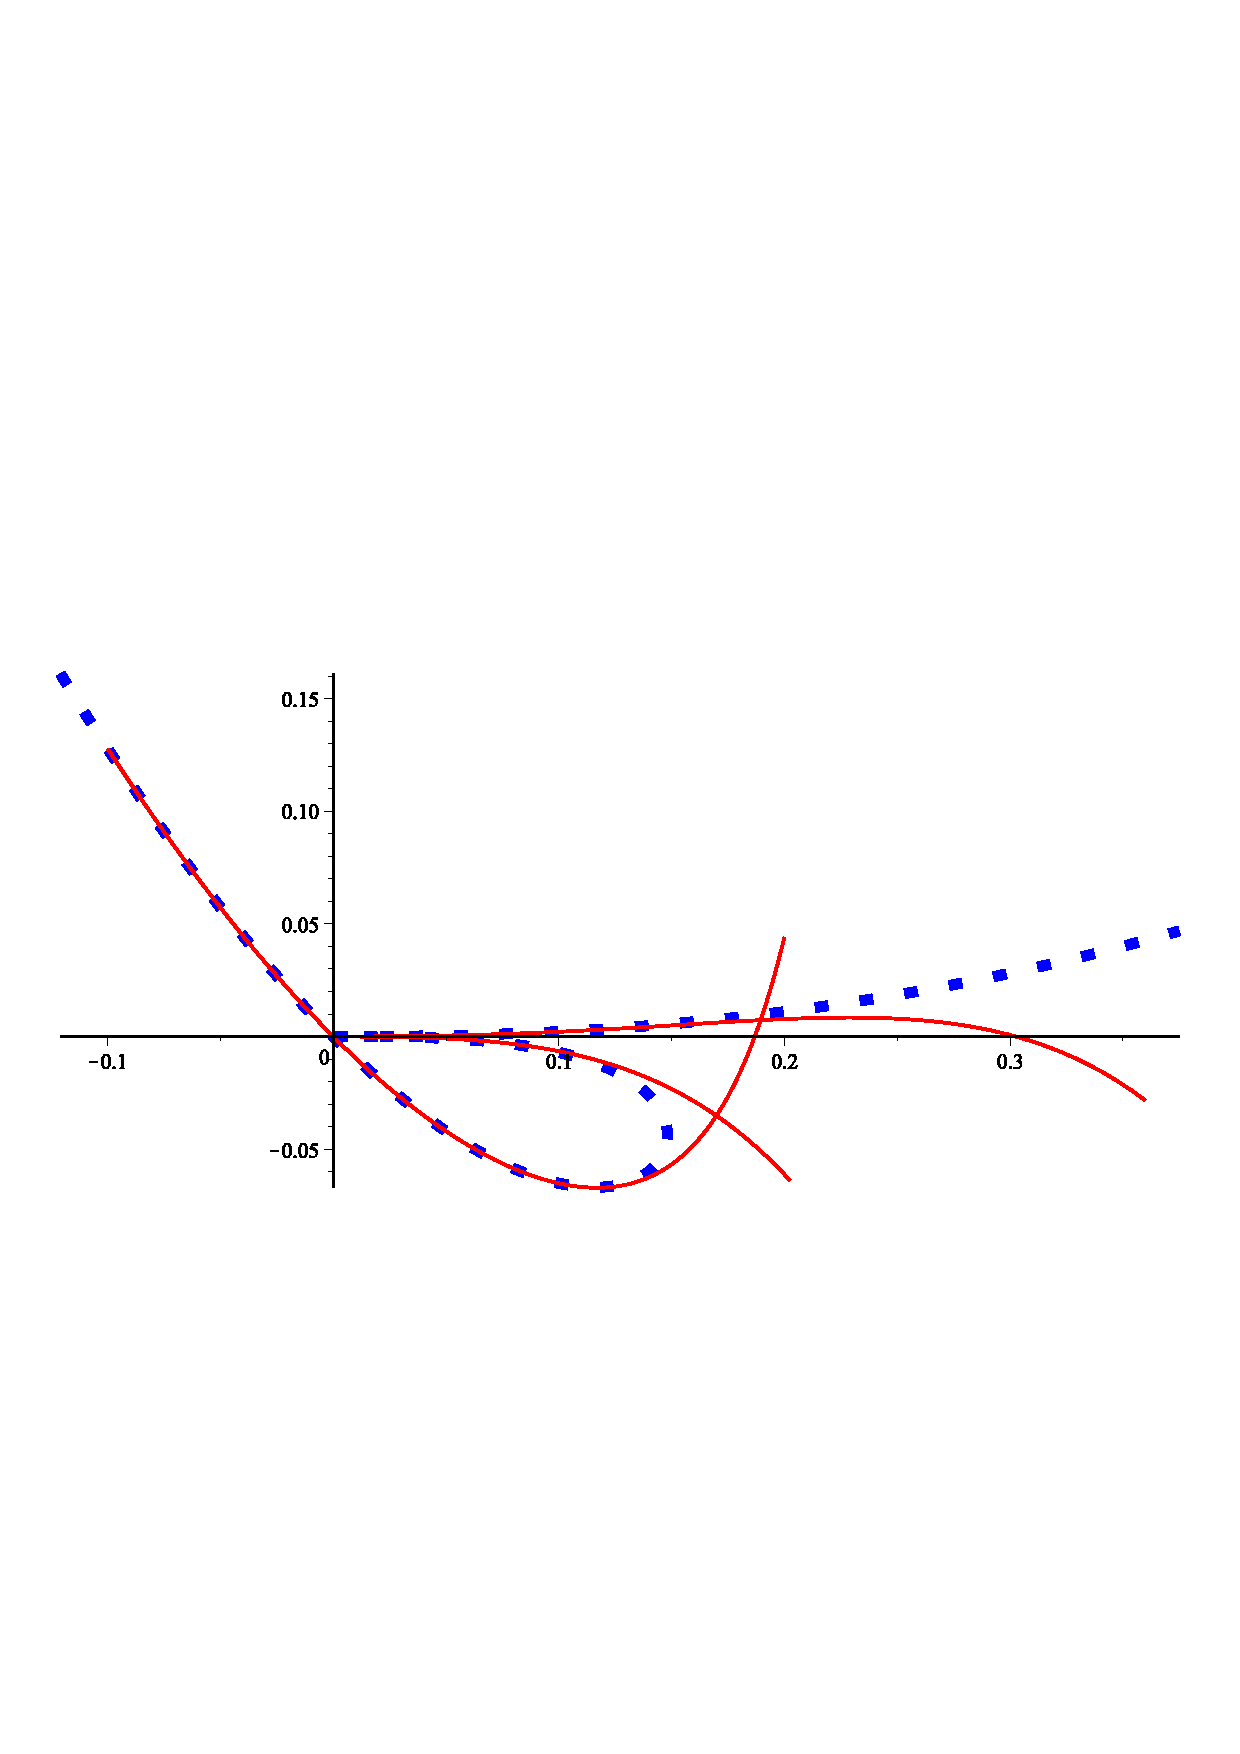
\includegraphics[scale=0.35]{Export/kurvorplot2d1.png}
\end{center}

\subsection{Exempel --- Byte av axel}

Ellipsen $\left(3 \sin(t), 2 \cos(t)\right)$ saknar singulariteter, men vi kan parametrisera om kurvan ändå. Notera hur omparametriseringarna skiljer från $t=0$ och $t=\pi$, jämfört med $t=\pm \pi/2$:

\begin{maplegroup}
\begin{verbatim}
> Reparametrize(3*sin(t), 2*cos(t), t, 0, 10, 0, false);

Elapsed Time: 0.015 s.
\end{verbatim}
\mapleresult
\begin{maplelatex}
\mapleinline{inert}{2d}{[t, 2-(1/9)*t^2-(1/324)*t^4-(1/5832)*t^6-(5/419904)*t^8-(7/7558272)*t^10]}{\[\displaystyle \left[t,2-1/9\,{t}^{2}-{\frac {{t}^{4}}{324}}-{\frac {{t}^{6}}{5832}}-{\frac {5\,{t}^{8}}{419904}}-{\frac {7\,{t}^{10}}{7558272}}\right]\]}
\end{maplelatex}
\end{maplegroup}

\begin{maplegroup}
\begin{verbatim}
> Reparametrize(3*sin(t), 2*cos(t), t, Pi, 10, 0, false);

Elapsed Time: 0.016 s.
\end{verbatim}
\mapleresult
\begin{maplelatex}
\mapleinline{inert}{2d}{[t, -2+(1/9)*t^2+(1/324)*t^4+(1/5832)*t^6+(5/419904)*t^8+(7/7558272)*t^10]}{\[\displaystyle \left[t,-2+1/9\,{t}^{2}+{\frac {{t}^{4}}{324}}+{\frac {{t}^{6}}{5832}}+{\frac {5\,{t}^{8}}{419904}}+{\frac {7\,{t}^{10}}{7558272}}\right]\]}
\end{maplelatex}
\end{maplegroup}

\begin{maplegroup}
\begin{verbatim}
> Reparametrize(3*sin(t), 2*cos(t), t, (1/2)*Pi, 10, 0, false);

Elapsed Time: 0.016 s.
\end{verbatim}
\mapleresult
\begin{maplelatex}
\mapleinline{inert}{2d}{[3-(3/8)*t^2-(3/128)*t^4-(3/1024)*t^6-(15/32768)*t^8-(21/262144)*t^10, t]}{\[\displaystyle \left[3-3/8\,{t}^{2}-{\frac {3\,{t}^{4}}{128}}-{\frac {3\,{t}^{6}}{1024}}-{\frac {15\,{t}^{8}}{32768}}-{\frac {21\,{t}^{10}}{262144}},t\right]\]}
\end{maplelatex}
\end{maplegroup}

\begin{maplegroup}
\begin{verbatim}
> Reparametrize(3*sin(t), 2*cos(t), t, -(1/2)*Pi, 10, 0, false);

Elapsed Time: 0.015 s.
\end{verbatim}
\mapleresult
\begin{maplelatex}
\mapleinline{inert}{2d}{[-3+(3/8)*t^2+(3/128)*t^4+(3/1024)*t^6+(15/32768)*t^8+(21/262144)*t^10, t]}{\[\displaystyle \left[-3+3/8\,{t}^{2}+{\frac {3\,{t}^{4}}{128}}+{\frac {3\,{t}^{6}}{1024}}+{\frac {15\,{t}^{8}}{32768}}+{\frac {21\,{t}^{10}}{262144}},t\right]\]}
\end{maplelatex}
\end{maplegroup}

\vspace{20pt}
Ritar vi sedan ut originalparametriseringen av kurvan tillsammans med de fyra omparametriseringarna får vi:

\begin{center}
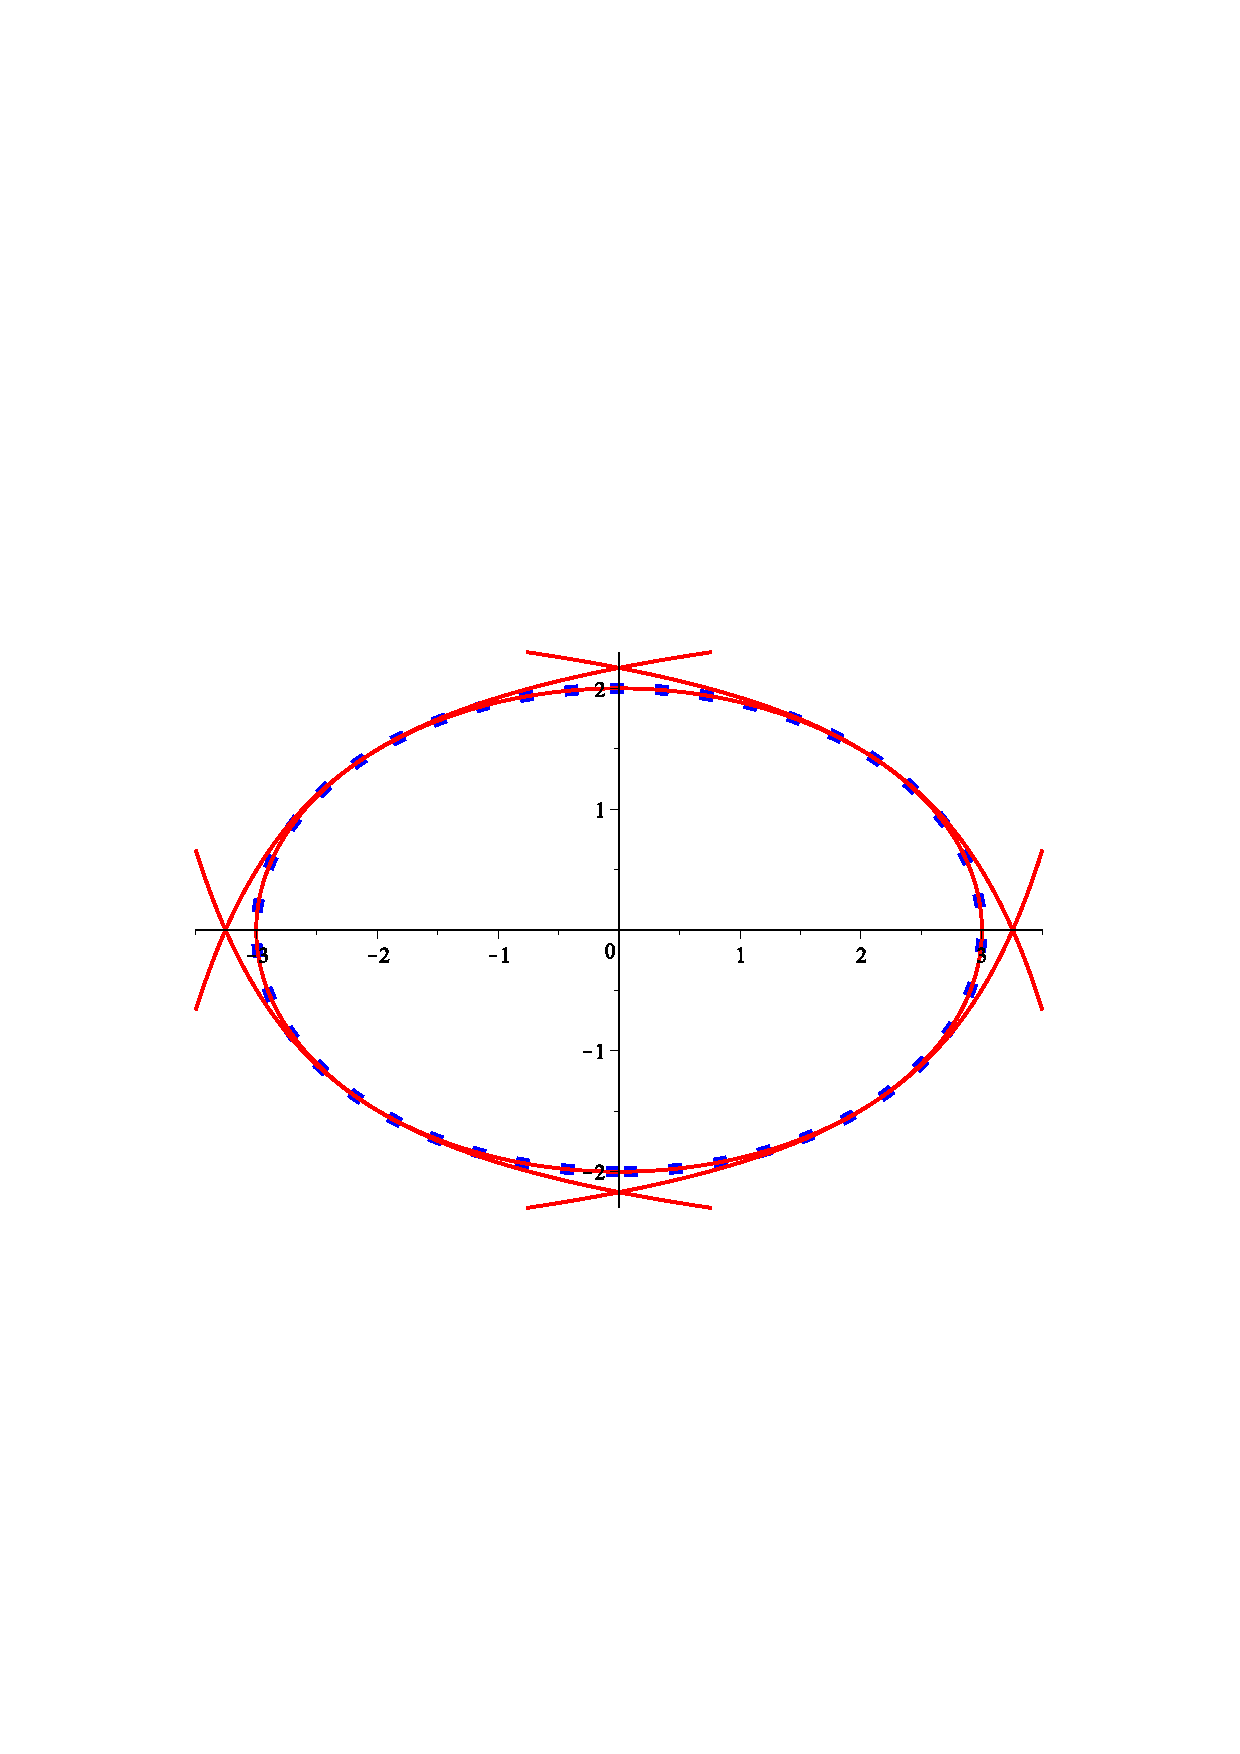
\includegraphics[scale=0.35]{Export/kurvorplot2d2.png}
\end{center}

\subsection{Exempel --- Singulariteter}
\label{ReparametrizeSingularities}

Kurvan $\left(t^3(t - 1)^3(t + 1)^3,t^5(t - 1)^2(t + 1)^2\right) = \left(t^9 - 3t^7 + 3t^5 - t^3, t^5 - 2t^7 + t^9\right)$ har en singularitet i $t = 0$ av ordning $2$, en i $t = 1$ av ordning $1$
och en i $t = -1$ av ordning $1$. Vi analyserar hur omparametriseringarna uppför sig i dessa tre singulariteter:

\begin{maplegroup}
\begin{verbatim}
> Reparametrize(t^3*(t-1)^3*(t+1)^3, t^5*(t-1)^2*(t+1)^2, t, 0, 15,
0, false);

Elapsed Time: 0.031 s.
\end{verbatim}
\mapleresult
\begin{maplelatex}
\mapleinline{inert}{2d}{[t^3, -1428*t^15-273*t^13-55*t^11-12*t^9-3*t^7-t^5]}{\[\displaystyle \left[{t}^{3},-1428\,{t}^{15}-273\,{t}^{13}-55\,{t}^{11}-12\,{t}^{9}-3\,{t}^{7}-{t}^{5}\right]\]}
\end{maplelatex}
\end{maplegroup}

\begin{maplegroup}
\begin{verbatim}
> Reparametrize(t^3*(t-1)^3*(t+1)^3, t^5*(t-1)^2*(t+1)^2, t, 1, 15, 
0, false);

Elapsed Time: 0.063 s.
\end{verbatim}
\mapleresult
\begin{maplelatex}
\mapleinline{inert}{2d}{[(1/2)*sqrt(4)*t^3-(9/4)*t^4+(207/64)*sqrt(4)*t^5-21*t^6+(150183/4096)*sqrt(4)*t^7-(137655/512)*t^8+(66893079/131072)*sqrt(4)*t^9-3978*t^10+(132735945771/16777216)*sqrt(4)*t^11-(8385901667/131072)*t^12+(70379121262905/536870912)*sqrt(4)*t^13-(4345965/4)*t^14+(78087826643607459/34359738368)*sqrt(4)*t^15, t^2]}{\[\displaystyle
\begin{array}{l}
\left[1/2\, \sqrt{4}{t}^{3}-9/4\,{t}^{4}+{\frac {207\, \sqrt{4}{t}^{5}}{64}}-21\,{t}^{6}+{\frac {150183\, \sqrt{4}{t}^{7}}{4096}}\right. \\
\mbox{}-{\frac {137655\,{t}^{8}}{512}}+{\frac {66893079\, \sqrt{4}{t}^{9}}{131072}}-3978\,{t}^{10}+{\frac {132735945771\, \sqrt{4}{t}^{11}}{16777216}}\\
\mbox{}-{\frac {8385901667\,{t}^{12}}{131072}}+{\frac {70379121262905\, \sqrt{4}{t}^{13}}{536870912}}\\
\left.\mbox{}-{\frac {4345965\,{t}^{14}}{4}}+{\frac {78087826643607459\, \sqrt{4}{t}^{15}}{34359738368}},{t}^{2}\right]
\end{array}\]}
\end{maplelatex}
\end{maplegroup}

\begin{maplegroup}
\begin{verbatim}
> Reparametrize(t^3*(t-1)^3*(t+1)^3, t^5*(t-1)^2*(t+1)^2, t, -1, 15, 
0, true);

Elapsed Time: 0.047 s.
\end{verbatim}
\mapleresult
\begin{maplelatex}
\mapleinline{inert}{2d}{[(1/2)*sqrt(4)*t^3+(9/4)*t^4+(207/64)*sqrt(4)*t^5+21*t^6+(150183/4096)*sqrt(4)*t^7+(137655/512)*t^8+(66893079/131072)*sqrt(4)*t^9+3978*t^10+(132735945771/16777216)*sqrt(4)*t^11+(8385901667/131072)*t^12+(70379121262905/536870912)*sqrt(4)*t^13+(4345965/4)*t^14+(78087826643607459/34359738368)*sqrt(4)*t^15, -t^2]}{\[\displaystyle
\begin{array}{l}
\left[1/2\, \sqrt{4}{t}^{3}+9/4\,{t}^{4}+{\frac {207\, \sqrt{4}{t}^{5}}{64}}+21\,{t}^{6}+{\frac {150183\, \sqrt{4}{t}^{7}}{4096}}\right.\\
\mbox{}+{\frac {137655\,{t}^{8}}{512}}+{\frac {66893079\, \sqrt{4}{t}^{9}}{131072}}+3978\,{t}^{10}+{\frac {132735945771\, \sqrt{4}{t}^{11}}{16777216}}\\
\mbox{}+{\frac {8385901667\,{t}^{12}}{131072}}+{\frac {70379121262905\, \sqrt{4}{t}^{13}}{536870912}}\\
\left.\mbox{}+{\frac {4345965\,{t}^{14}}{4}}+{\frac {78087826643607459\, \sqrt{4}{t}^{15}}{34359738368}},-{t}^{2}\right]
\end{array}\]}
\end{maplelatex}
\end{maplegroup}

\vspace{20pt}
Ritar vi sedan ut originalparametriseringen av kurvan tillsammans med de tre omparametriseringarna får vi följande intressanta bild:

\begin{center}
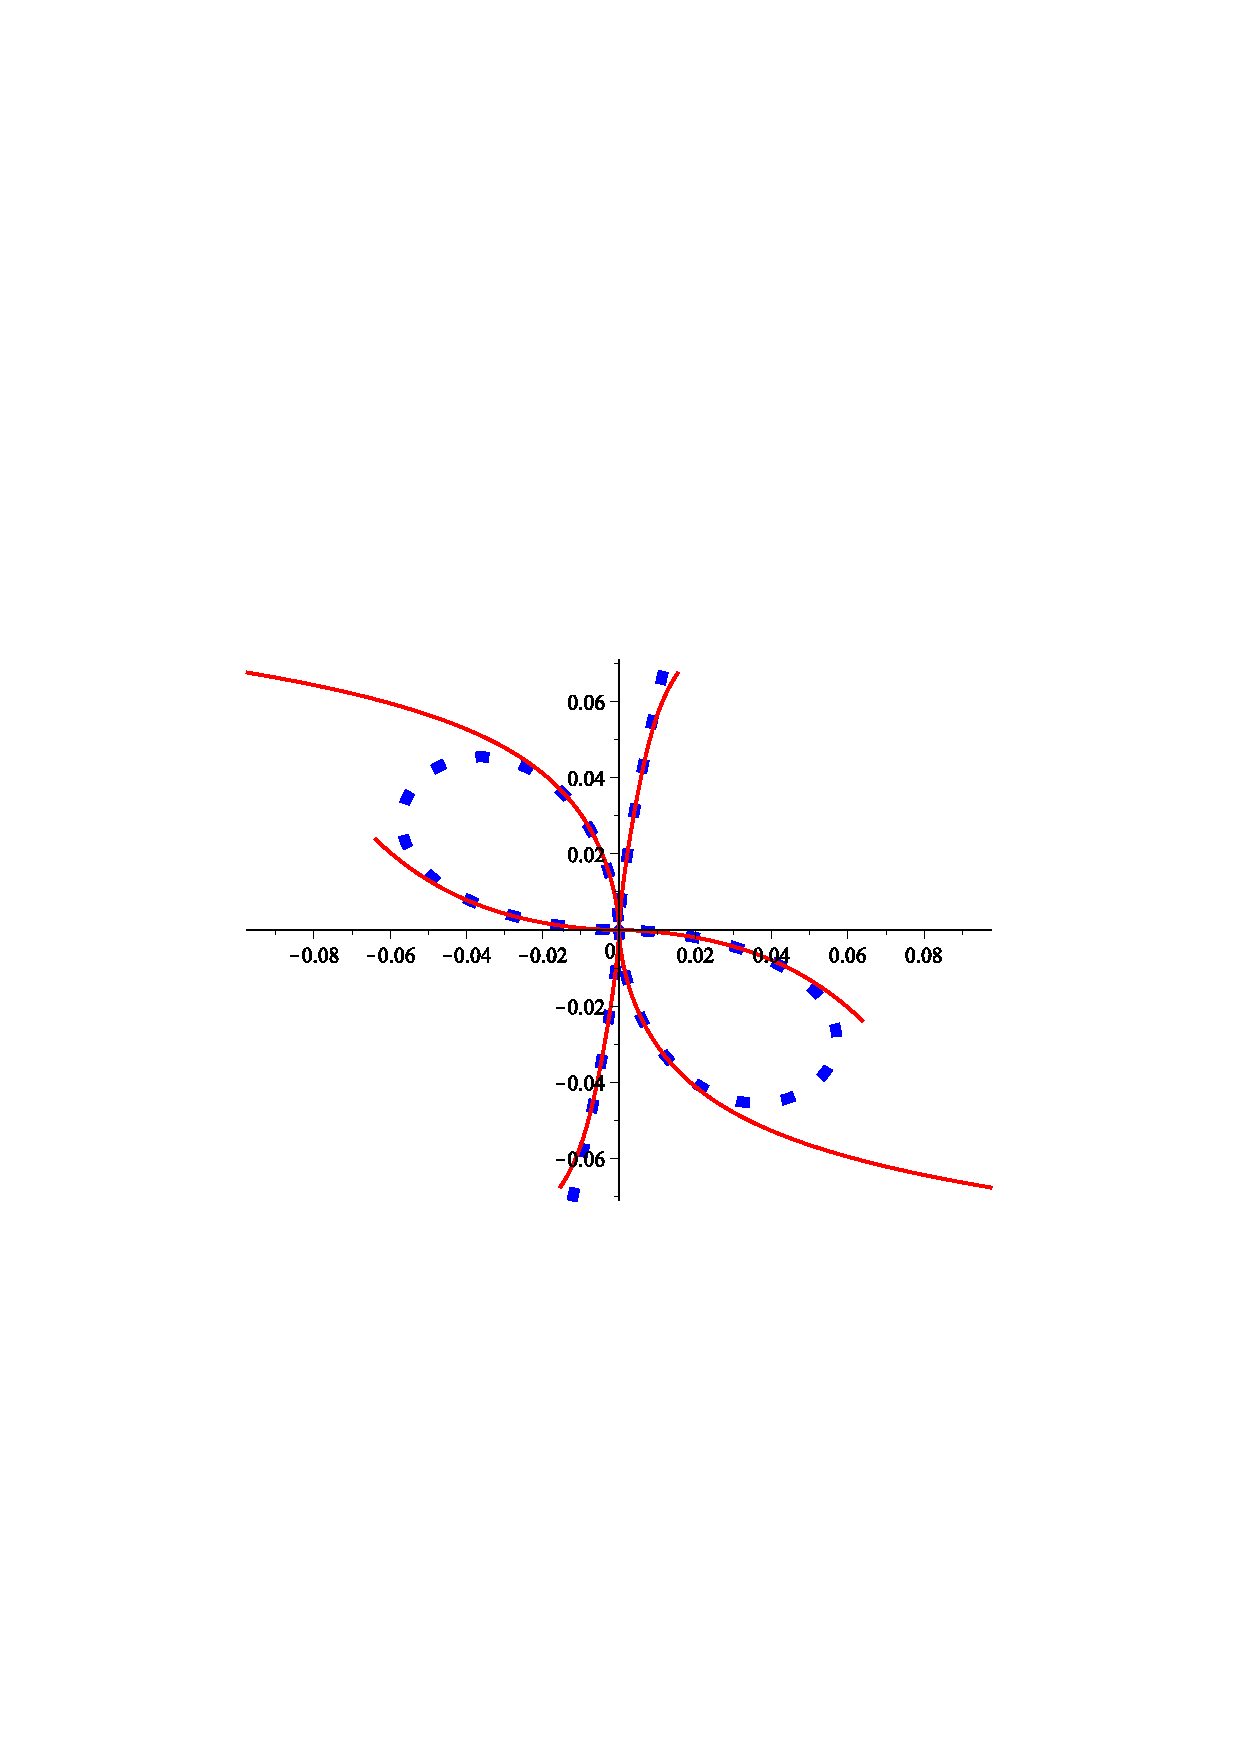
\includegraphics[scale=0.35]{Export/kurvorplot2d3.png}
\end{center}

\subsection{Exempel --- Negering}

Kurvan $\left(t^3 - t^2,t^3 + t^2\right)$ har en singularitet av ordning $1$ i $t = 0$. Vi använder Maple för att omparametrisera kurvan i denna punkt:

\begin{maplegroup}
\begin{verbatim}
> Reparametrize(t^3-t^2, t^3+t^2, t, 0, 10, 0, true);

Elapsed Time: 0.000 s.
\end{verbatim}
\mapleresult
\begin{maplelatex}
\mapleinline{inert}{2d}{[-t^2, 3*t^4+2*t^3+t^2+(21/4)*t^5+10*t^6+(1287/64)*t^7+42*t^8+(46189/512)*t^9+198*t^10]}{\[\displaystyle \left[-{t}^{2},3\,{t}^{4}+2\,{t}^{3}+{t}^{2}+{\frac {21\,{t}^{5}}{4}}+10\,{t}^{6}+{\frac {1287\,{t}^{7}}{64}}+42\,{t}^{8}+{\frac {46189\,{t}^{9}}{512}}+198\,{t}^{10}\right]\]}
\end{maplelatex}
\end{maplegroup}

\vspace{20pt}
Som man kan se av omparametriseringen blir x-termen $-t^2$. Man kan be Maple att omparametrisera kurvan så att x-termen blir positiv. Detta
medför givetvis att y-termen får komplexa koefficienter:

\begin{maplegroup}
\begin{verbatim}
> Reparametrize(t^3-t^2, t^3+t^2, t, 0, 10, 0, false);

Elapsed Time: 0.031 s.
\end{verbatim}
\mapleresult
\begin{maplelatex}
\mapleinline{inert}{2d}{[t^2, -t^2-(2*I)*t^3+3*t^4+(21/4*I)*t^5-10*t^6-(1287/64*I)*t^7+42*t^8+(46189/512*I)*t^9-198*t^10]}{\[\displaystyle
\begin{array}{l}
\left[{t}^{2},-{t}^{2}-2\,i{t}^{3}+3\,{t}^{4}+{\frac {21\,i}{4}}{t}^{5}\right.\\
\left.\mbox{}-10\,{t}^{6}-{\frac {1287\,i}{64}}{t}^{7}+42\,{t}^{8}+{\frac {46189\,i}{512}}{t}^{9}-198\,{t}^{10}\right]
\end{array}\]}
\end{maplelatex}
\end{maplegroup}

\vspace{20pt}
Om vi plottar den ursprungliga funktionen och dess reellvärda omparametrisering tillsammans med realdelen och imaginärdelen av den komplexa omparametriseringen var för sig (tunna punkt-streckade linjer), får vi följande graf:

\begin{center}
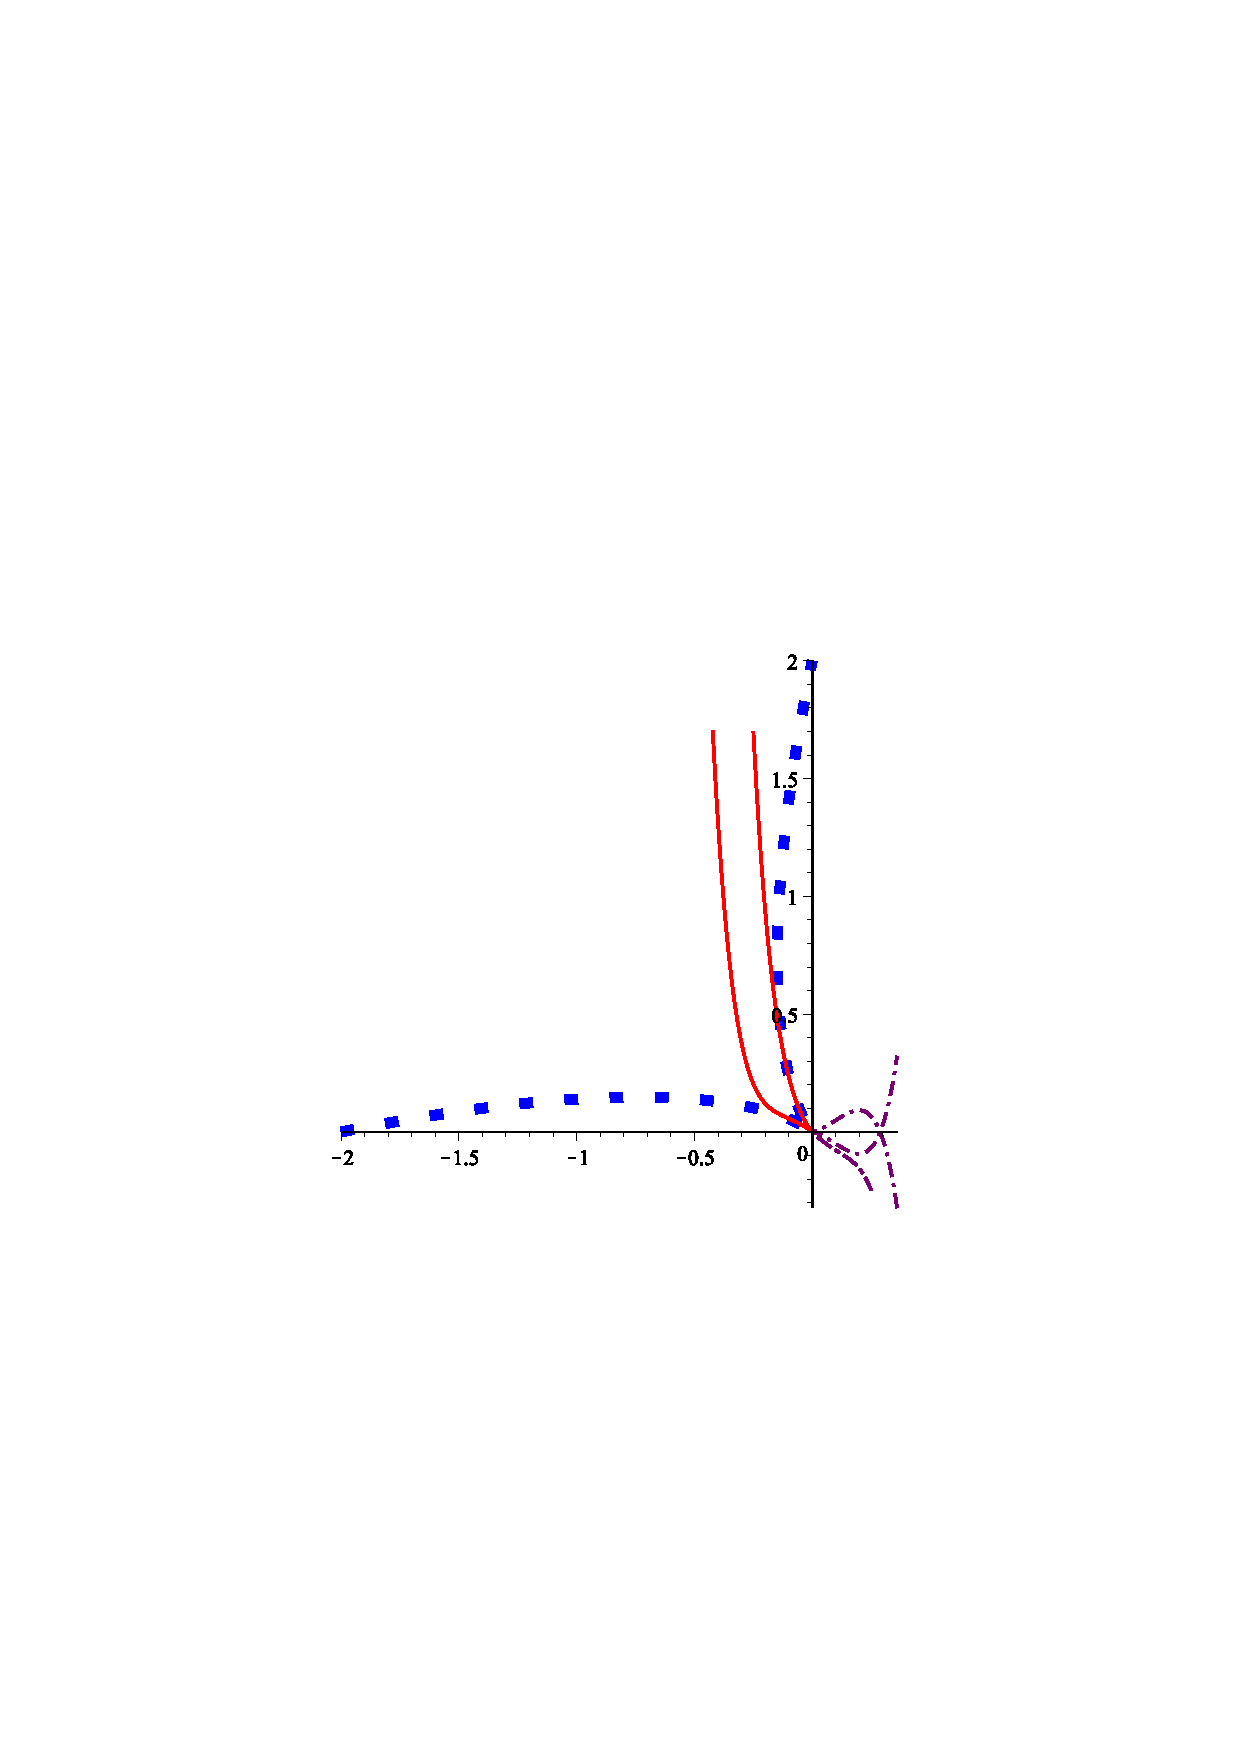
\includegraphics[scale=0.35]{Export/kurvorplot2d4.png}
\end{center}

\subsection{Exempel --- Udda ordning}

Kurvan $\left(t^4 - t^3,t^4 + t^3\right)$ har en singularitet av ordning $2$ i $t = 0$. Den liknar mycket kurvan i exemplet ovan, men eftersom ordningen av x- och y-termerna är udda ($3$), kommer omparametriseringen att vara reell utan att x-termen måste negeras. Vi använder Maple för att omparametrisera kurvan:

\begin{maplegroup}
\begin{verbatim}
> Reparametrize(t^4-t^3, t^4+t^3, t, 0, 10, 2, true);

Elapsed Time: 0.016 s.
\end{verbatim}
\mapleresult
\begin{maplelatex}
\mapleinline{inert}{2d}{[-t^3, 2*t^4+t^3+(8/3)*t^5+4*t^6+(520/81)*t^7+(2618/243)*t^8+(56/3)*t^9+(217360/6561)*t^10]}{\[\displaystyle \left[-{t}^{3},2\,{t}^{4}+{t}^{3}+8/3\,{t}^{5}+4\,{t}^{6}+{\frac {520\,{t}^{7}}{81}}+{\frac {2618\,{t}^{8}}{243}}+{\frac {56\,{t}^{9}}{3}}+{\frac {217360\,{t}^{10}}{6561}}\right]\]}
\end{maplelatex}
\end{maplegroup}

\vspace{20pt}
Vi kan också parametrisera om kurvan utan en negativ $t^n$ komponent. Eftersom ordningen hos komponenterna är udda, kommer bara de udda termerna byta tecken, och komplexa termer undvikas: 

\begin{maplegroup}
\begin{verbatim}
> Reparametrize(t^4-t^3, t^4+t^3, t, 0, 10, 0, false);

Elapsed Time: 0.015 s.
\end{verbatim}
\mapleresult
\begin{maplelatex}
\mapleinline{inert}{2d}{[t^3, 2*t^4-t^3-(8/3)*t^5+4*t^6-(520/81)*t^7+(2618/243)*t^8-(56/3)*t^9+(217360/6561)*t^10]}{\[\displaystyle \left[{t}^{3},2\,{t}^{4}-{t}^{3}-8/3\,{t}^{5}+4\,{t}^{6}-{\frac {520\,{t}^{7}}{81}}+{\frac {2618\,{t}^{8}}{243}}-{\frac {56\,{t}^{9}}{3}}+{\frac {217360\,{t}^{10}}{6561}}\right]\]}
\end{maplelatex}
\end{maplegroup}

\vspace{20pt}
Om vi plottar den ursprungliga kurvan och dess två parametriseringar (dessa två ger samma kurva), får vi följande graf:

\begin{center}
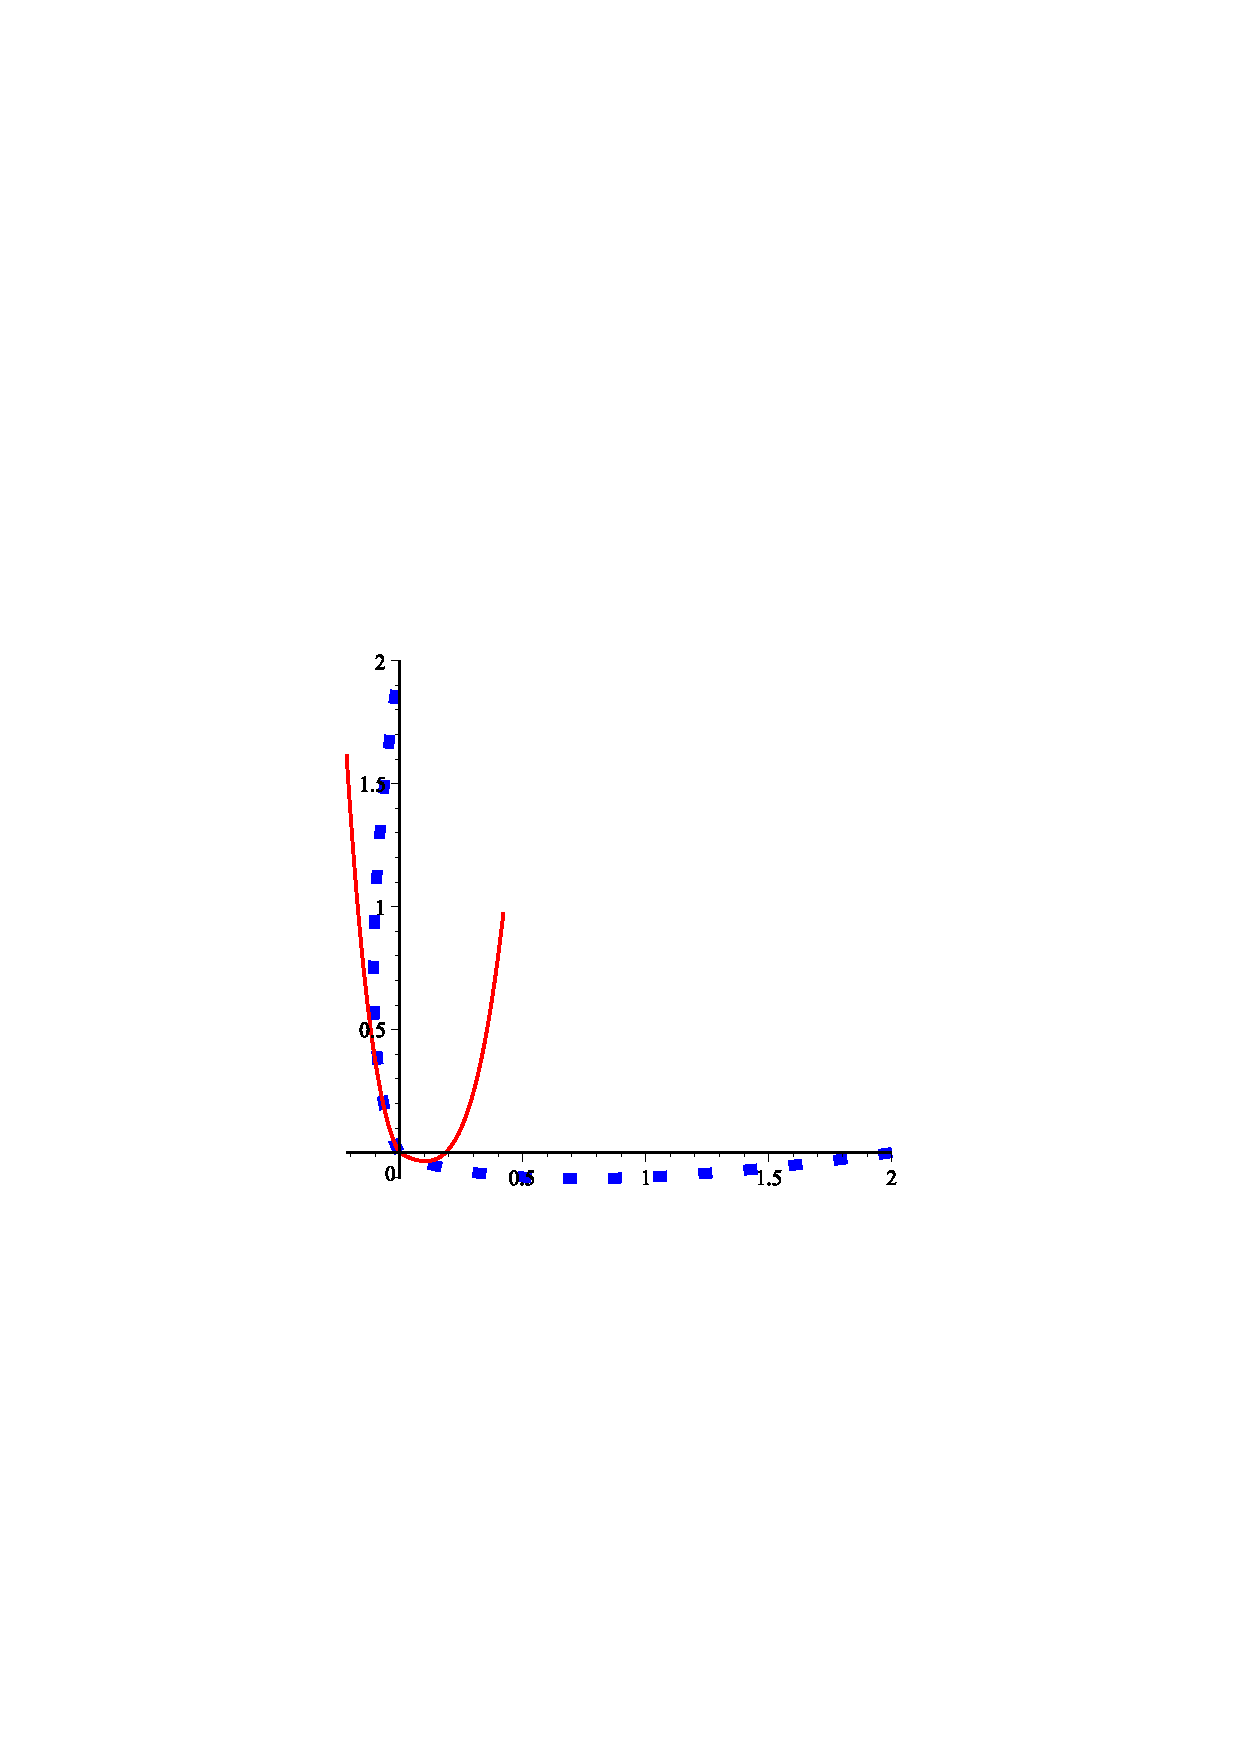
\includegraphics[scale=0.35]{Export/kurvorplot2d5.png}
\end{center}

\chapter[Källtexter --- Semigrupper]{Källtexter till Maple --- Semigrupper}
\label{Semigrupper}

\section{FindGCD}

\emph{FindGCD}-funktionen beräknar den största gemensamma delaren (greatest common divisor) mellan två heltal $a$ och $b$. Den beräknar också de två heltalen $A$ och $B$, sådana att $\gcd = A a + B b$.

\begin{table}[h]
\caption{Parametrar för \emph{FindGCD}}
\begin{center}
\begin{tabular}{|l|l|}
\hline
$a$ & Det första heltalet. \\
$b$ & Det andra heltalet. \\
\hline
\end{tabular}
\end{center}
\end{table}

\begin{verbatim}
FindGCD := proc(a, b)
   local a0 , b0 , m, n, r, GCD, BList, Position, A, B, switch;

   if not type(a, integer) then
      ERROR("a must be an integer!", a)
   end if;

   if not type(b, integer) then
      ERROR("b must be an integer!", b)
   end if;

   if a < b then
      m := b; 
      n := a; 
      switch := true
   else
      m := a; 
      n := b; 
      switch := false
   end if;

   a0 := m;
   b0 := n;
   GCD := n;
   r := m mod n;
   Position := 1;

   while r <> 0 do
      BList[Position] := -(m - r)/n;
      Position := Position + 1;
      m := n;
      n := r;
      GCD := r;
      r := m mod n
   end do;

   A := 0;
   B := 1;

   while 1 < Position do
      Position := Position - 1;
      r := B;
      B := A + BList[Position] * B;
      A := r
   end do;

   if switch then
      RETURN([GCD, B, A])
   else
      RETURN([GCD, A, B])
   end if
end proc
\end{verbatim}

\subsection{Exempel}

Följande exempel beräknar den största gemensamma delaren för 12312334 och 239487192:

\begin{verbatim}
> FindGCD(12312334,239487192);
\end{verbatim}
\[\left[2, -1065409, 54774\right]\]

Resultatet blir $2$. Dessutom får vi:
\[2 = 12312334 \cdot (-1065409) + 239487192 \cdot 54774\]

\section{FindGCDList}

\emph{FindGCDList}-funktionen beräknar den största gemensamma delaren (greatest common divisor) för en lista med heltal. Den returnerar också en lista med heltal sådana att summan av koefficienterna i den ursprungliga heltalslistan multiplicerat med motsvarande koefficienter i den returnerade listan blir lika med den största gemensamma delaren.

\begin{table}[h]
\caption{Parametrar för \emph{FindGCDList}}
\begin{center}
\begin{tabular}{|l|l|}
\hline
$IntegerList$ & En lista med heltal. \\
\hline
\end{tabular}
\end{center}
\end{table}

\begin{verbatim}
FindGCDList := proc(IntegerList)
   local NrIntegers, Position, GCD, Coefficients, l;

   if not type(IntegerList, list) then
      ERROR("IntegerList must be a list of integers!", 
         IntegerList)
   end if;

   NrIntegers := nops(IntegerList);
   if NrIntegers < 1 then
      ERROR("IntegerList must be a list of at least one integer!", 
         IntegerList)
   elif NrIntegers = 1 then
      RETURN([IntegerList1, [1]])
   end if;

   l := FindGCD(IntegerList[1], IntegerList[2]);
   GCD := l[1];
   Coefficients := [l[2], l[3]];
   Position := 3;

   while Position <= NrIntegers do
      l := FindGCD(GCD, IntegerList[Position]);
      GCD := l[1];
      Coefficients := [op(Coefficients * l[2]), l[3]];
      Position := Position + 1
   end do;

   RETURN([GCD, Coefficients])
end proc
\end{verbatim}

\subsection{Exempel}

Följande exempel beräknar den största gemensamma delaren för 6, 9 och 20:

\begin{verbatim}
> FindGCDList([6,9,20]);
\end{verbatim}
\[\left[1, \left[-7, 7, -1\right]\right]\]

Från svaret kan man också utläsa att
\[1 = 6 \cdot (-7) + 9 \cdot 7 + 20 \cdot (-1)\]

\section{FindConductor}

\emph{FindConductor}-funktionen beräknar konduktören för en lista med heltal vars största gemensamma delare är 1. Sats \ref{S4} säger ju att en sådan finns (förutsatt att den största gemensamma delaren är 1).

\begin{table}[h]
\caption{Parametrar för \emph{FindConductor}}
\begin{center}
\begin{tabular}{|l|p{9cm}|}
\hline
$Generators$ & En lista med heltal, vars största gemensamma delare måste vara 1.\\
$PrintTime$ & En frivillig parameter. Om \emph{true} så skrivs tidsåtgången för beräkningen ut på skärmen.\\
\hline
\end{tabular}
\end{center}
\end{table}

\begin{verbatim}
FindConductor := proc(Generators)
   local Conductor, l, MinValue, NrGenerators, g, ZMin, GCD, 
      a, b, c, d, e, StartTime;

   StartTime := time();

   if not type(Generators, list) then
      ERROR("Generators must be a list of integers!", 
         Generators)
   end if;

   l := FindGCDList(Generators);
   if l[1] <> 1 then
      ERROR(cat("The Generators must not have a common ",
         "divisor greater than 1!"), [Generators, l[1]])
   end if;

   NrGenerators := nops(Generators);
   MinValue := min(op(Generators));
   ZMin := array(0..MinValue - 1);
   ZMin[0] := MinValue;

   for l from 1 to MinValue - 1 do
      ZMin[l] := 0
   end do;

   for l to NrGenerators do
      g := Generators[l];
      if g <> MinValue then
         GCD := gcd(g, MinValue);
         b := MinValue/GCD;
         for e from 0 to MinValue do
            if e = MinValue then
               c := 0
            elif ZMin[e] <> 0 then
               c := ZMin[e]
            else
               c := -1
            end if;

            if 0 <= c then
               for a to b do
                  c := c + g;
                  d := c mod MinValue;
                  if ZMin[d] = 0 or c < ZMin[d] then
                     ZMin[d] := c
                  end if
               end do
            end if
         end do
      end if
   end do;

   Conductor := ZMin[0];
   for a to MinValue - 1 do
      if Conductor < ZMin[a] then
         Conductor := ZMin[a]
      end if
   end do;

   Conductor := Conductor - MinValue + 1;

   if nargs = 1 or args[2] then
      printf("Elapsed Time: %0.3f s.\n", time() - StartTime)
   end if;

   RETURN(Conductor)
end proc
\end{verbatim}

\subsection{Exempel --- Explicit generalisering möjlig?}
\label{ConductorGeneralized}

För att se om vi kan generalisera formeln för beräkningen av konduktören för en numerisk semigrupp genererad av fler än två element, beräknar vi konduktören för $\left<2 \cdot 3 \cdot 5, 2 \cdot 3 \cdot 7, 2 \cdot 5 \cdot 7, 3 \cdot 5 \cdot 7\right> = \left<30, 42, 70, 105\right>$:

\begin{verbatim}
> FindConductor([2*3*5,2*3*7,2*5*7,3*5*7]);

Elapsed Time: 0.000 s.
\end{verbatim}
\[384\]

Konduktören blir i detta exempel $384 = 2^7 \cdot 3$. Som man kan se i detta exempel verkar det inte finnas någon enkel självklar generalisering av formeln för konduktören av $\left<m, n\right>$, då $m$ och $n$ är relativt prima ($c = (m-1)(n-1)$).

\subsection{Exempel --- Stor semigrupp}
\label{ExempelStorSemigrupp}

I följande exempel illustreras fördelen med att beräkningen av konduktören genomförs utan att motsvarande semigrupp genereras:

\begin{verbatim}
> FindConductor([2139,2398,3321]);

Elapsed Time: 8.062 s.
\end{verbatim}
\[277188\]

Konduktören för $\left<2139, 2398, 3321\right>$ är alltså $277188$, dvs. lite mer än 129 ggr större än den minsta generatorn ($2139$). Beräkningen av motsvarande semigrupp kommer att ta betydligt mer tid (326.313 s). Utskriften av semigruppen kan också krascha Maple (vilket den gjorde i mitt fall).

\section{FindSemiGroup}

\emph{FindSemiGroup}-funktionen genererar semigruppen från en lista med generatorer. Den returnerar konduktören och alla element fram till och med konduktören i semigruppen. Skulle inte generatorerna vara relativt prima (dvs. de har en största gemensam delare större än 1), delar den först generatorerna med den största gemensamma delaren, skapar motsvarande semigrupp, multiplicerar sedan elementen med den största gemensamma delaren och returnerar motsvarande ``konduktör'', den största gemensamma delaren, samt vilka element som ingår i semigruppen fram till och med ``konduktören''\footnote{Med ``konduktören'' i detta fall menas konduktören av semigruppen som genereras av generatorerna delat med den största gemensamma delaren, multiplicerat med den största gemensamma delaren.}.

\begin{table}[h]
\caption{Parametrar för \emph{FindSemiGroup}}
\begin{center}
\begin{tabular}{|l|p{9cm}|}
\hline
$Generators$ & En lista med heltal.\\
$PrintTime$ & En frivillig parameter. Om \emph{true} så skrivs tidsåtgången för beräkningen ut på skärmen.\\
\hline
\end{tabular}
\end{center}
\end{table}

\begin{verbatim}
FindSemiGroup := proc(Generators)
   local Conductor, l, GCD, Generators2, MinValue, NrGenerators, 
   g, ZMin, GCD2,a, b, c, d, e, SemiGroup, StartTime;

   StartTime := time();

   if not type(Generators, list) then
      ERROR("Generators must be a list of integers!", Generators)
   end if;

   l := FindGCDList(Generators);
   GCD := l[1];
   if GCD = 1 then
      Generators2 := Generators
   else
      Generators2 := Generators/GCD
   end if;

   NrGenerators := nops(Generators2);
   MinValue := min(op(Generators2));
   ZMin := array(0..MinValue - 1);
   ZMin[0] := MinValue;

   for l from 1 to MinValue - 1 do
      ZMin[l] := 0
   end do;

   for l to NrGenerators do
      g := Generators2[l];
      if g <> MinValue then
         GCD2 := gcd(g, MinValue);
         b := MinValue/GCD2;

         for e from 0 to MinValue do
            if e = MinValue then
               c := 0
            elif ZMin[e] <> 0 then
               c := ZMin[e]
            else
               c := -1
            end if;

            if 0 <= c then
               for a to b do
                  c := c + g;
                  d := c mod MinValue;

                  if ZMin[d] = 0 or c < ZMin[d] then
                     ZMin[d] := c
                  end if
               end do
            end if
         end do
      end if
   end do;

   Conductor := ZMin[0];
   for a to MinValue - 1 do
      if Conductor < ZMin[a] then
         Conductor := ZMin[a]
      end if
   end do;

   Conductor := Conductor - MinValue + 1;
   ZMin := array(1..Conductor);
   for l to Conductor do
      ZMin[l] := 0
   end do;

   for l to NrGenerators do
      g := Generators2[l];

      for a to Conductor + 1 do
         if Conductor < a then
            b := g
         elif ZMin[a] <> 0 then
            b := ZMin[a] + g
         else
            b := 0
         end if;

         if 0 < b then
            while b <= Conductor do
               ZMin[b] := b;
               b := b + g
            end do
         end if
      end do
   end do;

   SemiGroup := {};

   for a to Conductor do
      if 0 < ZMin[a] then
         SemiGroup := SemiGroup union {ZMin[a]}
      end if
   end do;

   if GCD <> 1 then
      SemiGroup := GCD * SemiGroup
   end if;

   if nargs = 1 or args2 then
      printf("Elapsed Time: %0.3f s.\n", time() - StartTime)
   end if;

   RETURN([Conductor * GCD, SemiGroup])
end proc
\end{verbatim}

\subsection{Exempel --- Enkel semigrupp}

Det första exemplet beräknar $\left<15, 10, 6\right>$:

\begin{verbatim}
> FindSemiGroup([15,10,6]);

Elapsed Time: .000 s.
\end{verbatim}
\[\left[30, \left\{6, 10, 12, 15, 16, 18, 20, 21, 22, 24, 25, 26, 27, 28, 30\right\}\right]\]

Vi får att konduktören är $30$ och att 
\[\left<15, 10, 6\right> = \left\{6, 10, 12, 15, 16, 18, 20, 21, 22, 24, 25, 26, 27, 28, 30, \ldots\right\}\]
där ``\ldots'' betyder ``alla heltal som kommer därefter''.

\subsection{Exempel --- $\gcd \neq 1$}

Detta exempel beräknar $\left<30, 20, 12\right>$:

\begin{verbatim}
> FindSemiGroup([30,20,12]);

Elapsed Time: .000 s.
\end{verbatim}
\[\left[60, 2 \left\{6, 10, 12, 15, 16, 18, 20, 21, 22, 24, 25, 26, 27, 28, 30\right\}\right]\]

Eftersom den största gemensamma delaren av 30, 20 och 12 är 2 (vilket även ses i resultatet) kan vi uttyda att
\[\left<30, 20, 12\right> = 2 \cdot \left\{6, 10, 12, 15, 16, 18, 20, 21, 22, 24, 25, 26, 27, 28, 30, \ldots\right\}\]

Multiplikationen av 2 med hela mängden skall läsas som att varje element i mängden skall multipliceras med 2.

\subsection{Exempel --- Lite större semigrupp}

Vi kan också beräkna lite större semigrupper. I detta exempel beräknas $\left<21, 93, 32\right>$:

\begin{verbatim}
> FindSemiGroup([21,93,32]);

Elapsed Time: .000 s.
\end{verbatim}
\[
\begin{array}{ll}
\left[332\right., & \left\{21, 32, 42, 53, 63, 64, 74, 84, 85, 93, 95, 96, 105, 106,\right. \\
&	114, 116, 117, 125, 126, 127, 128, 135, 137, 138, 146, 147, 148, 149,\\
&	156, 157, 158, 159, 160, 167, 168, 169, 170, 177, 178, 179, 180, 181,\\
&	186, 188, 189, 190, 191, 192, 198, 199, 200, 201, 202, 207, 209, 210,\\
&	211, 212, 213, 218, 219, 220, 221, 222, 223, 224, 228, 230, 231, 232,\\
&	233, 234, 239, 240, 241, 242, 243, 244, 245, 249, 250, 251, 252, 253,\\
&	254, 255, 256, 260, 261, 262, 263, 264, 265, 266, 270, 271, 272, 273,\\
&	274, 275, 276, 277, 279, 281, 282, 283, 284, 285, 286, 287, 288, 291,\\
&	292, 293, 294, 295, 296, 297, 298, 300, 302, 303, 304, 305, 306, 307,\\
&	308, 309, 311, 312, 313, 314, 315, 316, 317, 318, 319, 320, 321, 323,\\
&	\left.\left.324, 325, 326, 327, 328, 329, 330, 332\right\}\right]\end{array}
\]

Som man kan se växer semigruppen ganska fort. Det kan vara en bra idé att först kolla vad konduktören till en semigrupp är, innan själva semigruppen beräknas. Annars kan man riskera att krascha Maple. Exemplet i \ref{ExempelStorSemigrupp} är ett exempel på en sådan semigrupp.

\subsection{Exempel --- generalisering av formel?}

I detta exempel beräknar vi semigruppen som definierades i exempel \ref{ConductorGeneralized} i beskrivningen av \emph{FindConductor}-funktionen. Notera att det normalt tar längre tid att beräkna semigruppen än konduktören, även om det inte är synligt i just detta exempel.

\begin{verbatim}
FindSemiGroup([2*3*5,2*3*7,2*5*7,3*5*7]);

Elapsed Time: .000 s.
\end{verbatim}
\[
\begin{array}{ll}
\left[384\right., & \left\{30, 42, 60, 70, 72, 84, 90, 100, 102, 105, 112, 114, 120, 126,\right\}\\
&	130, 132, 135, 140, 142, 144, 147, 150, 154, 156, 160, 162, 165, 168,\\
&	170, 172, 174, 175, 177, 180, 182, 184, 186, 189, 190, 192, 195, 196,\\
&	198, 200, 202, 204, 205, 207, 210, 212, 214, 216, 217, 219, 220, 222,\\
&	224, 225, 226, 228, 230, 231, 232, 234, 235, 237, 238, 240, 242, 244,\\
&	245, 246, 247, 249, 250, 252, 254, 255, 256, 258, 259, 260, 261, 262,\\
&	264, 265, 266, 267, 268, 270, 272, 273, 274, 275, 276, 277, 279, 280,\\
&	282, 284, 285, 286, 287, 288, 289, 290, 291, 292, 294, 295, 296, 297,\\
&	298, 300, 301, 302, 303, 304, 305, 306, 307, 308, 309, 310, 312, 314,\\
&	315, 316, 317, 318, 319, 320, 321, 322, 324, 325, 326, 327, 328, 329,\\
&	330, 331, 332, 333, 334, 335, 336, 337, 338, 339, 340, 342, 343, 344,\\
&	345, 346, 347, 348, 349, 350, 351, 352, 354, 355, 356, 357, 358, 359,\\
&	360, 361, 362, 363, 364, 365, 366, 367, 368, 369, 370, 371, 372, 373,\\
&	\left.\left.374, 375, 376, 377, 378, 379, 380, 381, 382, 384\right\}\right]
\end{array}
\]

\section{FindSemiGroupFromPolynomialRing}
\label{FindSemiGroupFromPolynomialRing}
Funktionen \emph{FindSemiGroupFromPolynomialRing} beräknar en serie generatorer för semigruppen motsvarande polynomringen $\mathbb{C}\left[g_1, \ldots, g_n\right]$, där $g_i$ är polynomen som anges i parameter 1 när man anropar funktionen. Semigruppen består av alla de heltal $n : \exists f \in \mathbb{C}\left[g_1, \ldots, g_n\right] : n = \mathbf{o}(f)$. Detta kan skrivas enklare som $\mathbf{o}(\mathbb{C}\left[g_1, \ldots, g_n\right])$.

\begin{table}[h]
\caption{Parametrar för \emph{FindSemiGroupFromPolynomialRing}}
\begin{center}
\begin{tabular}{|l|p{9cm}|}
\hline
$Polynomials$ & En lista med polynom.\\
$Variable$ & Namnet på variabeln.\\
$PrintTime$ & En frivillig parameter. Om \emph{true} så skrivs tidsåtgången för beräkningen ut på skärmen.\\
$PrintFormulae$ & En frivillig parameter. Om \emph{true} så skrivs för varje generator en explicit formel för hur motsvarande polynom genererats.\\
$MaxPolynomials$ & En frivillig parameter. Om den anges, anger den det maximala antalet polynom som kan genereras av algoritmen, innan den ger upp i sitt sökande efter lösningen. Om den inte anges, antas 5000 polynom vara gränsen.\\
\hline
\end{tabular}
\end{center}
\end{table}

\begin{verbatim}
FindSemiGroupFromPolynomialRing := proc(PolynomialGenerators, 
   Variable)
   local StartTime, GCD, Conductor, Polynomials, NrPolynomials,
      MaxPolynomials, Generators, PolynomialsByOrder, Orders,
      ExplicitNotation, FirstExplicitNotation, 
      NrOriginalPolynomials, OriginalOrders, MaxExponent, 
      MinOrder, HighestOrder, CalcExplicit, MaxTerm, MaxTerms, 
      a, b, c, d, e, f, g, h, e1, e2, g1, g2, g3, d1, d2, d3, p;

   StartTime := time();

   CalcExplicit := 4 <= nargs and args[4];

   if 5 <= nargs then
      MaxPolynomials:=args[5]
   else
      MaxPolynomials:=5000
   end if;

   if not type(PolynomialGenerators, list) then
      ERROR(cat("PolynomialGenerators must be a list of ",
         "polynomials!"), PolynomialGenerators)
   end if;

   NrOriginalPolynomials := nops(PolynomialGenerators);
   if NrOriginalPolynomials = 0 then
      ERROR("List of polynomials cannot be empty!")
   end if;

   f := PolynomialGenerators;
   for a to NrOriginalPolynomials do
      g1 := f[a];
      if not type(g1, polynom) then
         ERROR(cat("PolynomialGenerators must be a list of ",
            "polynomials!"), PolynomialGenerators)
      end if;

      ExplicitNotation[a] := p[a];
      OriginalOrders[a] := ldegree(g1, Variable);
      Orders[a] := OriginalOrders[a]
   end do;

   for a from 2 to NrOriginalPolynomials do
      for b to a - 1 do
         if Orders[a] < Orders[b] then
            c := Orders[a];
            Orders[a] := Orders[b];
            Orders[b] := c;
            c := f[a];
            f[a] := f[b];
            f[b] := c;
            c := ExplicitNotation[a];
            ExplicitNotation[a] := ExplicitNotation[b];
            ExplicitNotation[b] := c
         end if
      end do
   end do;

   MinOrder := Orders[1];
   GCD := MinOrder;
   Generators := [MinOrder];
   g1 := f[1];
   e := coeff(g1, Variable, MinOrder);
   Polynomials[1] := g1/e;
   ExplicitNotation[1] := ExplicitNotation[1]/e;
   g := 1;

   for a from 2 to NrOriginalPolynomials do
      g1 := f[a];
      b := ExplicitNotation[a];

      for h to g do
         g2 := Polynomials[h];
         d2 := ldegree(g2, Variable);
         e := coeff(g1, Variable, d2);

         if e <> 0 then
            g1 := g1 - e * g2;
            b := b - e * ExplicitNotation[h]
         end if
      end do;

      if g1 <> 0 then
         d := ldegree(g1, Variable);
         Generators := [op(Generators), d];
         GCD := gcd(GCD, d);
         e := coeff(g1, Variable, d);
         g1 := g1/e;
         b := b/e;
         g := g + 1;
         Polynomials[g] := g1;
         ExplicitNotation[g] := b;

         for h to g - 1 do
            g2 := Polynomials[h];
            e := coeff(g2, Variable, d);
            if e <> 0 then
               g2 := g2 - e * g1;
               Polynomials[h] := g2;
               ExplicitNotation[h] := ExplicitNotation[h] - e * b
            end if
         end do
      end if
   end do;

   NrPolynomials := g;
   if GCD = 1 then
      Conductor := FindConductor(Generators, false);
      MaxTerm := Variable^(Conductor+1);

      for c to NrOriginalPolynomials do
         MaxExponent[c] := ceil((Conductor + 1)/OriginalOrders[c])
      end do
   else
      Conductor := infinity
   end if;

   HighestOrder := max(op(Generators));
   for a from MinOrder to HighestOrder do
      PolynomialsByOrder[a] := 0
   end do;

   for a to NrPolynomials do
      f := Polynomials[a];
      d := ldegree(f, Variable);
      Orders[a] := d;
      PolynomialsByOrder[d] := a;
      FirstExplicitNotation[d] := ExplicitNotation[a]
   end do;

   a := 1;
   while a <= NrPolynomials do
      g1 := Polynomials[a];
      d1 := Orders[a];

      if g1 <> 0 and d1 <= Conductor then
         if CalcExplicit then
            e1 := ExplicitNotation[a]
         end if;

         b := 1;
         while b <= a do
            if b = a then
               g2 := g1;
               d2 := d1
            else
               g2 := Polynomials[b];
               d2 := Orders[b]
            end if;

            if g2 <> 0 and d2 <= Conductor then
               d := sort(simplify(expand(g1 * g2)));
               if CalcExplicit then
                  e2 := expand(e1 * ExplicitNotation[b])
               end if;

               d3 := d1 + d2;
               while d3 <= HighestOrder and d3 <= Conductor and 
                  d <> 0 and PolynomialsByOrder[d3] <> 0 do
                  
                  c := PolynomialsByOrder[d3];
                  g3 := Polynomials[c];

                  if g3 = 0 then
                     ERROR("Runtime Error", d)
                  end if;

                  e := coeff(d, Variable, d3);
                  d := d - e * g3;

                  if CalcExplicit then
                     e2 := e2 - e * ExplicitNotation[c]
                  end if;

                  d3 := ldegree(d, Variable)
               end do;

               if d <> 0 and d3 <= Conductor then
                  e := coeff(d, Variable, d3);
                  d := d/e;

                  if CalcExplicit then
                     e2 := e2/e
                  end if;

                  Generators := [op(Generators), d3];
                  GCD := gcd(GCD, d3);

                  if GCD = 1 and Conductor = infinity then
                     Conductor := FindConductor(Generators, false);

                     if Conductor < d3 then
                        Conductor := d3
                     end if;

                     for c to NrOriginalPolynomials do
                        MaxExponent[c] := ceil((Conductor + 1)/
                           OriginalOrders[c]);
                        MaxTerms[c] := p[c]^MaxExponent[c]
                     end do;

                     MaxTerm := Variable^(Conductor+1);
                     if Conductor < degree(d, Variable) then
                        d := rem(d, MaxTerm, Variable);
                        if CalcExplicit then
                           for c to NrOriginalPolynomials do
                              if MaxExponent[c] < 
                                 degree(e2, p[c]) then
                                 e2 := expand(rem(e2, 
                                    MaxTerms[c], p[c]))
                              end if
                           end do
                        end if
                     end if;

                     for c to NrPolynomials do
                        e := Polynomials[c];
                        if e <> 0 and 
                           Conductor < degree(e, Variable) then
                           
                           Polynomials[c] := rem(e, MaxTerm, 
                              Variable);

                           if CalcExplicit then
                              if Polynomials[c] = 0 then
                                 ExplicitNotation[c] := 0
                              end if
                           else
                              e := ExplicitNotation[c];
                              for f to NrOriginalPolynomials do
                                 if MaxExponent[f] < 
                                    degree(e, p[f]) then
                                    
                                    e := expand(rem(e, 
                                       MaxTerms[f], p[f]))
                                 end if
                              end do;

                              ExplicitNotation[c] := e
                           end if
                        end if
                     end do
                  elif Conductor < degree(d, Variable) then
                     d := rem(d, MaxTerm, Variable);
                     if CalcExplicit then
                        for c to NrOriginalPolynomials do
                           if MaxExponent[c] < 
                              degree(e2, p[c]) then
                              e2 := expand(rem(e2, 
                                 MaxTerms[c], p[c]))
                           end if
                        end do
                     end if
                  end if;

                  NrPolynomials := NrPolynomials + 1;
                  if NrPolynomials > MaxPolynomials then
                     ERROR(cat("Generated more polynomials than",
                        "allowed. Solution not found."),
                        MaxPolynomials)
                  end if;

                  Polynomials[NrPolynomials] := d;
                  Orders[NrPolynomials] := d3;

                  if CalcExplicit then
                     ExplicitNotation[NrPolynomials] := e2;
                     FirstExplicitNotation[d3] := e2
                  end if;

                  if HighestOrder < d3 then
                     HighestOrder := HighestOrder + 1;
                     while HighestOrder < d3 do
                        PolynomialsByOrder[HighestOrder] := 0;
                        HighestOrder := HighestOrder + 1
                     end do
                  end if;

                  PolynomialsByOrder[d3] := NrPolynomials;
                  h := NrPolynomials - 1;

                  for c to h do
                     e := Polynomials[c];
                     if e <> 0 then
                        f := coeff(e, Variable, d3);
                        if f <> 0 then
                           e := e - f * d;
                           NrPolynomials := NrPolynomials + 1;
                           if NrPolynomials > 
                              MaxPolynomials then
                              ERROR(cat("Generated more ",
                                 "polynomials than allowed. ",
                                 "Solution not found."),
                                 MaxPolynomials)
                           end if;

                           g := Orders[c];
                           Polynomials[NrPolynomials] := e;
                           Orders[NrPolynomials] := g;
                           PolynomialsByOrder[g] := 
                              NrPolynomials;

                           if CalcExplicit then
                              e := ExplicitNotation[c] - 
                                 f * e2;
                              ExplicitNotation[
                                 NrPolynomials] := e
                           end if;

                           Polynomials[c] := 0
                        end if
                     end if
                  end do
               end if
            end if;

            b := b + 1
         end do
      end if;

      a := a + 1
   end do;

   if Conductor = infinity then
      ERROR("No upper bound found.", PolynomialGenerators)
   end if;

   Generators := sort(Generators);
   a := {};
   b := [];
   for c to nops(Generators) do
      d := Generators[c];
      if d <= Conductor and not member(d, a) then
         b := [op(b), d];
         e := d;
         f := {};
         while e <= Conductor do
            f := f union {e};

            for h to nops(a) do
               g := a[h] + e;
               if g <= Conductor then 
                  f := f union {g}
               end if
            end do;

            e := e + d
         end do;

         a := a union f
      end if
   end do;

   Generators := b;
   if CalcExplicit then
      for c to NrOriginalPolynomials do
         MaxExponent[c] := ceil((Conductor + 1)/OriginalOrders[c]);
         MaxTerms[c] := p[c]^MaxExponent[c]
      end do;

      MaxTerm := Variable^(Conductor+1);

      for a to nops(Generators) do
         b := Generators[a];
         c := FirstExplicitNotation[b];

         for e to NrOriginalPolynomials do
            c := expand(rem(c, MaxTerms[e], p[e]))
         end do;

         d := convert(c, list);
         if 1 < nops(d) then
            for e to nops(d) do
               f := d[e];

               for g to NrOriginalPolynomials do
                  f := subs(p[g] = PolynomialGenerators[g], f)
               end do;

               if b < ldegree(f) then 
                  c := c - d[e] 
               end if
            end do
         end if;

         d := c;
         for g to NrOriginalPolynomials do
            d := subs(p[g] = PolynomialGenerators[g], d)
         end do;

         d := sort(expand(d));
         e := lcm(denom(c), denom(d));
         c := sort(e * c);
         d := sort(e * d);
         print(c = d)
      end do
   end if;

   if nargs < 3 or args[3] then
      printf("Elapsed Time: %0.3f s.\n", time() - StartTime)
   end if;

   RETURN(Generators)
end proc
\end{verbatim}

\subsection{Exempel --- Enkelt första exempel}
\label{SimplePolynomialRingExample}

I följande exempel beräknar vi den numeriska semigruppen $G_1$ motsvarande polynomringen $\mathbb{C}\left[t^4 + t^5, t^6 + t^7\right]$:

\begin{verbatim}
> FindSemiGroupFromPolynomialRing([t^4+t^5,t^6+t^7],t,true,true);
\end{verbatim}
\[\begin{array}{c}
p_1 = t^5 + t^4\\[3pt]
p_2 = t^7 + t^6\\[3pt]
p_1^3 - p_2^2 = t^{15} + 2 t^{14} + t^{13}\\
\end{array}\]
\begin{verbatim}
Elapsed Time: .000 s.
\end{verbatim}
\[\left[4, 6, 13\right]\]
\begin{verbatim}
> FindSemiGroup([4,6,13]);

Elapsed Time: 0.000 s.
\end{verbatim}
\[\left[16, \left\{4, 6, 8, 10, 12, 13, 14, 16\right\}\right]\]

Vi fick alltså att $G_1 = \left<4, 6, 13\right>=\left\{4, 6, 8, 10, 12, 13, 14, 16, \ldots\right\}$. Konduktören för semigruppen är 16. Vi fick dessutom veta att 13 kommer från $p_1^3 - p_2^2 = t^{15} + 2 t^{14} + t^{13}$, där $p_1 = t^5 + t^4$ och $p_2 = t^7 + t^6$.

Vi kan också jämföra detta resultat med den numeriska semigruppen som motsvarar polynomringen vi får om vi först gör en omparametrisering av kurvan i punkten $t = 0$:

\begin{verbatim}
> Reparametrize(t^4+t^5,t^6+t^7,t,0,15,0,false);

Elapsed Time: 0.047 s.
\end{verbatim}
\[
\begin{array}{l}
\left[t^4, t^6+\frac{1}{2}*t^7+\frac{1}{2}t^8+\frac{39}{64}t^9+\frac{105}{128}t^{10}+\frac{4807}{4096}t^{11}+\frac{7}{4}t^{12}+\right.\\[8pt]
\left.\frac{352495}{131072}t^{13}+\frac{138567}{32768}t^{14}+\frac{113591595}{16777216}t^{15}\right]\\
\end{array}
\]

\begin{verbatim}
> FindSemiGroupFromPolynomialRing([t^4,t^6 + 1/2*t^7 + 1/2*t^8 + 
   39/64*t^9 + 105/128*t^10 + 4807/4096*t^11 + 7/4*t^12 + 
   352495/131072*t^13 + 138567/32768*t^14 + 
   113591595/16777216*t^15],t,true,true);
\end{verbatim}

\[p_1=t^4\]
\[
\begin{array}{rcl}
16777216 p_2 & = & 113591595 t^{15} + 70946304 t^{14} + 45119360 t^{13} +\\[3pt]
& + & 29360128 t^{12} + 19689472 t^{11} + 13762560 t^{10} +\\[3pt]
 & + & 10223616 t^9 + 8388608 t^8 + 8388608 t^7 + 16777216 t^6\\[3pt]
\end{array}\]
\[
\begin{array}{l}
-281474976710656 p_1^3 + 281474976710656 p_2^2 =\\[3pt]
\qquad 12903050454644025 t^{30} + 16117807661429760 t^{29} +\\[3pt]
\qquad 15283738186818816 t^{28} + 13072231199539200 t^{27} +\\[3pt]
\qquad 10674858838319104 t^{26} + 8569833185345536 t^{25} +\\[3pt]
\qquad 6914209094303744 t^{24} + 5754492897198080 t^{23} +\\[3pt]
\qquad 5214414567374848 t^{22} + 6901048593612800 t^{21} +\\[3pt]
\qquad 4222124650659840 t^{20} + 2618276488151040 t^{19} +\\[3pt]
\qquad 1650916709105664 t^{18} + 1063090305105920 t^{17} +\\[3pt]
\qquad 703687441776640 t^{16} + 483785116221440 t^{15} +\\[3pt]
\qquad 351843720888320 t^{14} + 281474976710656 t^{13}\\
\end{array}
\]

\begin{verbatim}
Elapsed Time: 0.015 s.
\end{verbatim}
\[\left[4, 6, 13\right]\]

Från detta ser vi inte bara att den numeriska semigruppen är oförändrad vid omparametriseringen. Vi kan även notera att generatorn 13 genereras på samma sätt i båda fallen:
\[\mathbf{o}(p_1^3 - p_2^2) = 13\]

\subsection{Exempel --- Beräkningsintensivitet}
\label{CostRingExample}

Följande exempel är mer beräkningsintensivt. Vi skall beräkna den numeriska semigruppen $G_2$ motsvarande $\mathbb{C}\left[t^8 + t^{11}, t^{12} + t^{13}\right]$. För att se skillnaden i tidsåtgång mellan att endast beräkna generatorerna till semigruppen och att dessutom beräkna motsvarande polynom, gör vi två exekveringar enligt följande:

\begin{verbatim}
> FindSemiGroupFromPolynomialRing([t^11+t^8, t^13+t^12], t);

Elapsed Time: 1.078 s.
\end{verbatim}
\[\left[8, 12, 25\right]\]

\begin{verbatim}
> FindSemiGroupFromPolynomialRing([t^11+t^8, t^13+t^12], t, 
     true, true);
\end{verbatim}
\[p_1 = t^{11} + t^8 \]
\[p_2 = t^{13} + t^{12} \]
\[-p_1^3+p_2^2 = -t^{33}-3t^{30}-3t^{27}+t^{26}+2t^{25}\]
\begin{verbatim}
Elapsed Time: 4.671 s.
\end{verbatim}
\[\left[8, 12, 25\right]\]

\begin{verbatim}
> FindSemiGroup([8,12,25]);

Elapsed Time: 0.016 s.
\end{verbatim}
\[
\begin{array}{l}
\left[80, \left\{8, 12, 16, 20, 24, 25, 28, 32, 33, 36, 37, 40, 41, 44, 45, 48, 49, 50, 52, 53,\right.\right.\\
\left.\left.56, 57, 58, 60, 61, 62, 64, 65, 66, 68, 69, 70, 72, 73, 74, 75, 76, 77, 78, 80\right\}\right]\\
\end{array}
\]

Vi fick alltså att $G_2 = \left<8, 12, 25\right>$. Konduktören för semigruppen är 80. Vi fick dessutom veta att 25 kommer från $-p_1^3 +p_2^2 = -t^{33}-3t^{30}-3t^{27}+t^{26}+2t^{25}$, där $p_1 = t^{11} + t^8$ och $p_2 = t^{13} + t^{12}$.

För att förstå varför detta exempel är så beräkningsintensivt i jämförelse med exempel \ref{SimplePolynomialRingExample} betraktar vi förhållandet mellan konduktörerna och den lägsta av generatorerna i varje exempel. I Exempel \ref{SimplePolynomialRingExample} är den lägsta generatorn 4 och konduktören 16. Dvs. den största potens av denna generator som kan förekomma i algoritmen är 4. I detta exempel däremot, är den lägsta generatorn 8 men konduktören är 80. Detta betyder att den högsta potensen av denna generator som förekommer i algoritmen är 10. Antalet kombinationer av generatorerna är i detta exempel mycket större, varför algoritmen måste generera betydligt fler polynom innan den är klar. Dessutom växer polynomen i takt med att större potenser förekommer i dem. Detta gör polynommultiplikationer kostbara m.a.p. tidsåtgång. Att denna faktor är betydande ser man i detta senare exempel. Vi beräknar semigruppen två gånger, först beräknas bara generatorerna, sedan även polynom motsvarande dessa generatorer. Eftersom komplexiteten är densamma i de två anropen ser vi att polynomaritmetiken i det senare fallet gjorde att funktionsanropet tog flera gånger längre tid att beräknas.

För att avsluta exemplet, undersöker vi vad som händer om vi först gör en
omparametrisering av kurvan:

\begin{verbatim}
> Reparametrize(t^8+t^11,t^12+t^13,t,0,20,2,false);

Elapsed Time: 0.062 s.
\end{verbatim}
\[\left[t^8, t^{13}+t^{12}-\frac{3}{2}t^{15}-\frac{13}{8}t^{16}+\frac{39}{16}t^{18}+\frac{351}{128}t^{19}\right]\]

\begin{verbatim}
> FindSemiGroupFromPolynomialRing([t^8, t^12 + t^13-3/2*t^15-
     13/8*t^16+39/16*t^18+351/128*t^19],t,true,true);
\end{verbatim}
\[p_1 = t^8\]
\[128p_2 = 351t^{19}+312t^{18}-208t^{16}-192t^{15}+128t^{13}+128t^{12}\]
\[
\begin{array}{rcl}
-16384p_1^3+16384p_2^2 & = & 123201t^{38}+219024t^{37}+97344t^{36}-\\
& - & 146016t^{35}-264576t^{34}-119808t^{33}+\\
& + & 133120t^{32}+249600t^{31}+116736t^{30}-\\
& - & 53248t^{29}-102400t^{28}-49152t^{27}+\\
& + & 16384t^{26}+32768t^{25}\\
\end{array}
\]
\begin{verbatim}
Elapsed Time: 4.000 s.
\end{verbatim}
\[\left[8, 12, 25\right]\]

Även i detta exempel förblir semigruppen oförändrad. Dessutom fås generatorerna på samma sätt: $\mathbf{o}(p_1^3 - p_2^2) = 25$.

\subsection{Exempel --- Flera polynom}

Följande enkla exempel visar att vi kan använda fler än två polynom som indata. Vi skall beräkna den numeriska semigruppen $G_3$ motsvarande $\mathbb{C}\left[t^5, t^7, t^{12} + t^{13}\right]$:

\begin{verbatim}
> FindSemiGroupFromPolynomialRing([t^5,t^7,t^12+t^13],t,
     true,true);
\end{verbatim}
\[p_1 = t^5\]
\[p_2 = t^7\]
\[-p_1 p_2 + p_3 = t^{13}\]
\begin{verbatim}
Elapsed Time: 0.016 s.
\end{verbatim}
\[\left[5, 7, 13\right]\]

\begin{verbatim}
> FindSemiGroup([5,7,13]);

Elapsed Time: 0.000 s.
\end{verbatim}
\[\left[17, \left\{5, 7, 10, 12, 13, 14, 15, 17\right\}\right]\]

Vi fick alltså att $G_3 = \left<5, 7, 13\right>=\left\{5, 7, 10, 12, 13, 14, 15, 17, \ldots\right\}$. Konduktören för semigruppen är 17. Vi fick dessutom veta att 13 kommer från $-p_1 p_2 + p_3 = t^{13}$, där $p_1 = t^5$, $p_2 = t^7$ och $p_3 = t^{12} + t^{13}$.

\subsection{Exempel --- Längre kedjor}

Här är ett annat enkelt litet exempel som visar att kedjan för att hitta generatorerna kan vara litet längre. Vi skall beräkna den numeriska semigruppen $G_4$ motsvarande $\mathbb{C}\left[t^4, t^6 + t^8 + t^{11}\right]$.

\begin{verbatim}
> FindSemiGroupFromPolynomialRing([t^4,t^6+t^8+t^11],
     t,true,true);
\end{verbatim}
\[p_1 = t^4\]
\[p_2 = t^{11}+t^8+t^6\]
\[p_1^4-p_1^3-2p_1^2 p_2+p_2^2 = t^{22}+2t^{17}\]
\begin{verbatim}
Elapsed Time: 0.000 s.
\end{verbatim}
\[\left[4, 6, 17\right]\]

\begin{verbatim}
> FindSemiGroup([4,6,17]);

Elapsed Time: 0.000 s.
\end{verbatim}
\[\left[20, \left\{4, 6, 8, 10, 12, 14, 16, 17, 18, 20\right\}\right]\]

Vi får att $G_4 = \left<4, 6, 17\right>=\left\{4, 6, 8, 10, 12, 14, 16, 17, 18, 20, \ldots\right\}$. Konduktören för semigruppen är 20. Vi fick dessutom veta att generatorn 17 kommer från $p_1^4 -p_1^3 - 2 p_1^2 p_2 +p_2^2 = t^{22} + 2 t^{17}$, där $p_1 = t^4$ och $p_2 = t^{11} +t^8 +t^6$.

\subsection{Exempel --- Andra enkel längre kedja}

Ett annat trivialt exempel: Här beräknas den numeriska semigruppen $G_5$ motsvarande $\mathbb{C}\left[t^2, t^4 + t^6 + t^{10} + t^{13}\right]$.

\begin{verbatim}
> FindSemiGroupFromPolynomialRing([t^2,t^4+t^6+t^10+t^13],
     t,true,true);
\end{verbatim}
\[p_1 = t^2\]
\[-p_1^5 - p_1^3 - p_1^2 + p_2 = t^{13}\]
\begin{verbatim}
Elapsed Time: 0.015 s.
\end{verbatim}
\[\left[2, 13\right]\]
\begin{verbatim}
> FindSemiGroup([2,13]);

Elapsed Time: 0.000 s.
\end{verbatim}
\[\left[12, \left\{2, 4, 6, 8, 10, 12\right\}\right]\]

Vi fick att $G_5 = \left<2, 13\right>=\left\{2, 4, 6, 8, 10, 12, \ldots\right\}$. Konduktören för semigruppen är 12 (dvs. mindre än den större generatorn). Vi fick dessutom veta att 13 kommer från $-p_1^5-p_1^3-p_1^2+p2 = t^{13}$, där $p_1 = t^2$ och $p_2 = t^4+t^6+t^{10}+t^{13}$.

\subsection{Exempel --- Avslutande exempel}

Här kommer ett litet besvärligare exempel: Vi ska beräkna den numeriska semigruppen $G_6$ motsvarande $\mathbb{C}\left[t^2 + t^5, t^4 + t^6 + t^{10} + t^{13}\right]$:

\begin{verbatim}
> FindSemiGroupFromPolynomialRing([t^2+t^5,
     t^4+t^6+t^10+t^13],t,true,true);
\end{verbatim}
\[p_1 = t^5+t^2\]
\[p_1^3+p_1^2-p_2 = t^{15}-t^{13}+3t^{12}+3t^9+2t^7\]
\begin{verbatim}
Elapsed Time: 0.000 s.
\end{verbatim}
\[\left[2, 7\right]\]
\begin{verbatim}
> FindSemiGroup([2,7]);

Elapsed Time: 0.000 s.
\end{verbatim}
\[\left[6, \left\{2, 4, 6\right\}\right]\]

Vi fick att $G_6 = \left<2, 7\right>=\left\{2, 4, 6,\ldots\right\}$. Konduktören för semigruppen är 6 (dvs. mindre än den större generatorn). Vi fick dessutom veta att 7 kommer från $p_1^3 + p_1^2 - p_2 = t^{15} - t^{13} + 3 t^{12} + 3 t^9 + 2 t^7$, där $p_1 = t^2 + t^5$ och $p_2 = t^4 + t^6 + t^{10} + t^{13}$.

För skojs skull gör vi även här en omparametrisering för att se dess motsvarande semigrupp, och hur generatorerna härleds:

\begin{verbatim}
> Reparametrize(t^5+t^2, t^13+t^10+t^6+t^4, t, 0, 10, 0, false);

Elapsed Time: 0.016 s.
\end{verbatim}
\[\left[t^2,7t^{10}-3t^9-2t^7+t^6+t^4\right]\]

\begin{verbatim}
> FindSemiGroupFromPolynomialRing([t^2,t^4+t^6-2*t^7
     -3*t^9+7*t^10],t,true,true);
\end{verbatim}
\[p_1 = t^2\]
\[p_1^3 + p_1^2 - p_2 = -7 t^{10} + 3 t^9 + 2 t^7\]
\begin{verbatim}
Elapsed Time: 0.000 s.
\end{verbatim}
\[\left[2, 7\right]\]

Återigen ser vi att semigruppen förblir oförändrad vid omparametrisering. Även generatorerna fås på samma sätt: $\mathbf{o}\left(p_1^3 + p_1^2 - p_2\right) = 7$.

\chapter[Källtexter --- Implicit notation]{Källtexter till Maple --- Implicit notation}
\label{FindImplicitNotation}

\section{FindImplicitNotation}

\emph{FindImplicitNotation}-funktionen beräknar den implicita notationen för en kurva, $C=\left\{(x,y)\in \mathbb{C}^2 : F(x,y)=0\right\}$ givet en explicit parametriserad version av samma kurva $C=C(\mathbb{R}), C(t)=(X_p(t),Y_p(t))$. För resultatet gäller att $F(X_p(t),Y_p(t))=0, \forall t \in \mathbb{R}$. Dessutom kommer $F(x,y)$ vara av minimal grad i den variabel som används för att definiera $X_p$ och $Y_p$. Funktionen tar också en maximal grad som används som övre gräns i sökalgoritmen, för att begränsa sökningen ifall resultat inte hittas.

\begin{table}[h]
\caption{Parametrar för \emph{FindImplicitNotation}}
\begin{center}
\begin{tabular}{|l|p{9cm}|}
\hline
$X_p$ & Parametriseringen av x-koordinaten. \\
$Y_p$ & Parametriseringen av y-koordinaten. \\
$Variable$ & Vilken variabel som använts vid parametriseringen.\\
$MaxDegree$ & Maximal grad vid sökning efter medlemmar i $\left<X_p , Y_p\right>$.\\
$PrintTime$ & En frivillig parameter. Om \emph{true} så skrivs tidsåtgången för beräkningen ut på skärmen.\\
\hline
\end{tabular}
\end{center}
\end{table}

\begin{verbatim}
FindImplicitNotation := proc(Xp, Yp, Variable, MaxDegree)
   local List, Pos, Count, ExpOrder, ExpOrders, MaxOrd, 
      Explicit, StartTime, CurrentMaxDegree, PrintTime, 
      Solution, i, j, k, f, g, p, x, y, a, b, c;

   StartTime := time();
   PrintTime := nargs < 5 or args[5];
   CurrentMaxDegree := MaxDegree;
   Solution := 0;
   f := Xp;
   g := Yp;

   if ldegree(f, Variable) = ldegree(g, Variable) then
      a := tcoeff(f, Variable);
      b := tcoeff(g, Variable);
      g := (g * a - f * b) / gcd(a,b)
   end if;

   List[0] := f;
   List[1] := g;
   Explicit[0] := x;
   Explicit[1] := y;
   MaxOrd := ldegree(f, Variable);
   ExpOrder[0] := MaxOrd;

   for i from 0 to MaxOrd - 1 do 
      ExpOrders[i] := -1 
   end do;

   ExpOrders[MaxOrd] := 0;
   j := ldegree(g, Variable);

   if MaxOrd < j then
      if MaxOrd + 1 < j then
         for i from MaxOrd + 1 to j - 1 do 
            ExpOrders[i] := -1 
         end do
      end if;

      MaxOrd := j
   end if;

   ExpOrders[j] := 1;
   ExpOrder[1] := j;
   Pos := 0;
   Count := 2;
   while Pos < Count do
      for i from 0 to Pos do
         if ExpOrder[Pos] + ExpOrder[i] <= CurrentMaxDegree then
            f := expand(List[Pos] * List[i]);
            p := expand(Explicit[Pos] * Explicit[i]);
            j := ldegree(f, Variable);
            k := 0;
            while j <= MaxOrd and f <> 0 do
               k := ExpOrders[j];
               if 0 <= k then
                  g := List[k];
                  a := tcoeff(g, Variable);
                  b := tcoeff(f, Variable);
                  c := gcd(a,b);
                  f := (f * a - g * b) / c;
                  p := p * a/c - Explicit[k] * b/c;
                  if f <> 0 then 
                     j := ldegree(f, Variable) 
                  end if
               else
                  List[Count] := f;
                  Explicit[Count] := p;
                  ExpOrder[Count] := j;
                  ExpOrders[j] := Count;
                  Count := Count + 1;
                  f := 0
               end if
            end do;

            if f <> 0 and MaxOrd < j then
               while MaxOrd < j - 1 do 
                  MaxOrd := MaxOrd + 1; 
                  ExpOrders[MaxOrd] := -1
               end do;

               List[Count] := f;
               Explicit[Count] := p;
               ExpOrder[Count] := j;
               ExpOrders[j] := Count;
               MaxOrd := j;
               Count := Count + 1
            elif 0 <= k and p <> 0 then
               j := degree(p);
               if j < CurrentMaxDegree then 
                  CurrentMaxDegree := j; 
                  Solution := p 
               end if
            end if
         end if
      end do;

      Pos := Pos + 1
   end do;

   if Solution = 0 then
      ERROR(cat("Implicit function not found. Please try ",
         "a higher Maximum Degree."), MaxDegree)
   end if;

   if PrintTime then 
      printf("Elapsed Time: %0.3f s.\n", time() - StartTime) 
   end if;

   a := [coeffs(Solution)];
   b := nops(a);
   j := op(1, a);

   for i from 2 to b do 
      j := gcd(j, op(i, a)) 
   end do;

   Solution := Solution/j;

   RETURN(sort(Solution) = 0)
end proc\end{verbatim}

\subsection{Exempel --- Elementärt första exempel}
\label{ImplicitNotationEx1}

Följande exempel beräknar den implicita funktionen till kurvan $C(t) =
\left(t^2, t^3\right)$:

\begin{verbatim}
> FindImplicitNotation(t^2,t^3,t,30,true);

Elapsed Time: 0.000 s.
\end{verbatim}
\[x^3 - y^2 = 0\]

Kurvan $C(t)$ motsvaras alltså av $x^3 - y^2 = 0$.

\begin{center}
\includegraphics[scale=0.35]{Export/implicitplot1.png}
\end{center}

Vi kan använda Maple för att rita ut både den explicita versionen av kurvan (prickad tjock linje) och den implicita versionen (tunn hel linje). Om vi inte övertygas av den algebraiska representationen, kan den visuella representationen snabbt ge oss en fingervisning hur väl den explicita och den implicita stämmer överens.

\subsection{Exempel --- Lite svårare}
\label{ImplicitNotationEx2}

Låt oss nu studera kurvan $C(t)=(t^2,t^3+t^4)$. Den ser till synes inte mycket svårare ut. Hur ser den implicita formen ut?

\begin{verbatim}
> FindImplicitNotation(t^2, t^3+t^4, t, 30, true);

Elapsed Time: 0.000 s.
\end{verbatim}
\[-x^4+x^3+2x^2y-y^2 = 0\]

Här behövs lite fler operationer genomföras för att $X_p(t)$ och $Y_p(t)$ ska ta ut varandra. I en graf ser de explicita och implicita formerna ut så här:

\begin{center}
\includegraphics[scale=0.35]{Export/implicitplot2.png}
\end{center}

\subsection{Exempel --- Annan variant på samma}
\label{ImplicitNotationEx3}

Nästa kurva är nästan identisk med föregående. Bara den andra potensen i t-koordinated är lite högre $C(t)=(t^2,t^3+t^7)$.

\begin{verbatim}
> FindImplicitNotation(t^2, t^3+t^7, t, 30, true);

Elapsed Time: 0.000 s.
\end{verbatim}
\[-x^7-2x^5-x^3+y^2 = 0\]

Komplexiteten är samma som föregående kurva. I en graf ser de explicita och implicita formerna ut så här:

\begin{center}
	\includegraphics[scale=0.35]{Export/implicitplot3.png}
\end{center}

\subsection{Exempel --- Jmfr. exempel \ref{SimplePolynomialRingExample}}

Detta exempel motsvarar exempel \ref{SimplePolynomialRingExample} till funktionen \emph{FindSemiGroupFromPolynomialRing}: $C(t)=\left(t^2+t^3,t^5+t^6\right)$.

\begin{verbatim}
> FindImplicitNotation(t^4+t^5, t^6+t^7, t, 40, true);

Elapsed Time: 0.000 s.
\end{verbatim}
\[-x^7+2x^4y^2-xy^4+y^5 = 0\]

I en graf ser de explicita och implicita formerna ut så här:

\begin{center}
	\includegraphics[scale=0.35]{Export/implicitplot4.png}
\end{center}

\subsection{Exempel --- Jmfr. exempel \ref{CostRingExample}}

Detta exempel motsvarar det lite mer beräkningskrävande exemplet \ref{CostRingExample} till funktionen \emph{FindSemiGroupFromPolynomialRing}: $C(t)=\left(t^8+t^{11},t^{12}+t^{13}\right)$.

\begin{verbatim}
> FindImplicitNotation(t^8+t^11, t^12+t^13, t, 150, true);

Elapsed Time: 0.438 s.
\end{verbatim}
\[
\begin{array}{l}
-x^{13}+4x^{10}y^2+5x^9y^3-42x^8y^4-11x^7y^5-6x^7y^4+33x^6y^5-\\
-85x^5y^6+125x^4y^7-14x^3y^8+25x^2y^9+y^{11}+4x^4y^6-25x^3y^7+\\
+36x^2y^8+13xy^9-3y^{10}-xy^8+3y^9 = 0
\end{array}
\]

I en graf ser de explicita och implicita formerna ut så här:

\begin{center}
\includegraphics[scale=0.35]{Export/implicitplot5.png}
\end{center}

\subsection{Exempel --- Jmfr. exempel \ref{ReparametrizeSingularities}}

Detta exempel motsvarar rosetten i exemplet \ref{ReparametrizeSingularities} till funktionen \emph{Reparametrize}: $C(t)=\left(t^3(t - 1)^3(t + 1)^3,t^5(t - 1)^2(t + 1)^2\right)$.

\begin{verbatim}
> FindImplicitNotation(t^3*(t-1)^3*(t+1)^3, t^5*(t-1)^2*(t+1)^2, 
     t, 150, true);

Elapsed Time: 1.266 s.
\end{verbatim}
\[
\begin{array}{l}
x^9-9x^8y+36x^7y^2-84x^6y^3+126x^5y^4-126x^4y^5+\\
+84x^3y^6-36x^2y^7+9xy^8-y^9+x^4y^3 = 0
\end{array}
\]

I en graf ser de explicita och implicita formerna ut så här:

\begin{center}
\includegraphics[scale=0.35]{Export/implicitplot6.png}
\end{center}

\chapter[Källtexter --- Multiplicitetsföljder]{Källtexter till Maple --- Multiplicitetsföljder}

\section{BlowUpXY}
\label{BlowUpXY}

\emph{BlowUpXY}-funktionen tar en funktion $F(x, y)$ med en singularitet i origo och blåser upp den i ytterligare en dimension ($z=y/x$). Därefter returneras multipliciteten $m$ av $F(x,y) = F(x, x \cdot z)$ samt den motsvarande uppblåsningen $F(x, x \cdot y)/{x^m}$. (Eftersom vi kommer använda \emph{BlowUpXY}-funktionen flera gånger i rad väljer vi dock att kalla variabeln för den nya dimensionen för $y$ istället för $z$, för att slippa hitta på nya variabelnamn i varje steg.)

\begin{table}[h]
\caption{Parametrar för \emph{BlowUpXY}}
\begin{center}
\begin{tabular}{|l|p{9cm}|}
\hline
$F$ & Funktion i två variabler med singularitet i origo. \\
$XVariable$ & Namnet på variabeln som motsvarar $x$.\\
$YVariable$ & Namnet på variabeln som motsvarar $y$.\\
\hline
\end{tabular}
\end{center}
\end{table}

\begin{verbatim}
BlowUpXY := proc(F, XVariable, YVariable)
   local G, m;

   G := subs(YVariable = XVariable * YVariable, F);
   m := ldegree(G, XVariable);

   RETURN([m, expand(G/XVariable^m)])
end proc
\end{verbatim}

\subsection{Exempel}

Följande är ett enkelt exempel på en uppblåsnin av $F(x,y)=y^2-x^5$:

\begin{verbatim}
> BlowUpXY(y^2-x^5,x,y)
\end{verbatim}
\[[2, -x^3+y^2]\]

\section{MultiplicitySequenceXY}
\label{MultiplicitySequenceXY}

\emph{MultiplicitySequenceXY}-funktionen beräknar multiplicitetsföljden av en algebraisk kurva givet på formen $F(x, y) = 0$, där $F \in \mathbb{C}\left[x, y\right]$ genom att upprepade gånger anropa \emph{BlowUpXY} tills den resulterande uppblåsningen blir reguljär.

\begin{table}[h]
\caption{Parametrar för \emph{MultiplicitySequenceXY}}
\begin{center}
\begin{tabular}{|l|p{9cm}|}
\hline
$F$ & Funktion i två variabler med singularitet i origo. \\
$XVariable$ & Namnet på variabeln som motsvarar $x$.\\
$YVariable$ & Namnet på variabeln som motsvarar $y$.\\
$PrintSteps$ & Frivillig parameter. Om \emph{true} skriver rutinen ut alla steg i beräkningen.\\
\hline
\end{tabular}
\end{center}
\end{table}

\begin{verbatim}
MultiplicitySequenceXY := proc(F, XVariable, YVariable)
   local M, m, G, resp;

   if coeff(F, YVariable, 0) = 0 then
      ERROR("Function not irreducible.", F )
   end if;

   m := infinity;
   M := [];
   G := F;

   while 1 <= m and degree(G)>0 do
      resp := BlowUpXY(G, XVariable, YVariable);
      m := resp[1];

      if G = resp[2] then 
         ERROR("Infinite loop.", G)
      end if;

      G := resp[2];

      if 0 < m then
         M := [op(M), m]
      end if;

      if 4 <= nargs then
         print([m, G])
      end if
   end do;

   RETURN(M)
end proc
\end{verbatim}

\subsection{Exempel --- Trivialt första exempel}
\label{MultiplicitySequenceXYEx1}

I detta exempel beräknas multiplicitetsföljden för $y^2 - x^5 = 0$:

\begin{verbatim}
> MultiplicitySequenceXY(y^2-x^5,x,y)
\end{verbatim}
\[\left[2, 2, 1\right]\]

Vill vi se de successiva uppblåsningarna gör vi som följer:

\begin{verbatim}
> MultiplicitySequenceXY(y^2-x^5,x,y,true)
\end{verbatim}
\[[2,-x^3+y^2]\]
\[[2,y^2-x]\]
\[[1,xy^2-1]\]
\[[0,x^3y^2-1]\]
\[\left[2, 2, 1\right]\]

Här ser vi att de successiva uppblåsningarna är $y^2-x^3$, $y^2-x$ och $xy^2-1$. Det sista steget är i sammanhangen irrelevant, då det bara används för att avsluta sekvensen. Sekvensen avslutas då en multiplicitet $m=0$ detekteras.

\subsection{Exempel --- Flera steg}
\label{MultiplicitySequenceXYEx2}

I detta exempel beräknas multiplicitetsföljden för $y^3 + x^2y - x^{11} = 0$:

\begin{verbatim}
> MultiplicitySequenceXY(y^3+x^2*y-x^11,x,y)
\end{verbatim}
\[[3, 1, 1, 1, 1, 1, 1, 1, 1]\]

\subsection{Exempel --- Högre multipliciteter}
\label{MultiplicitySequenceXYEx3}

I detta exempel beräknas multiplicitetsföljden för $y^5x+y^7+y^3x^3-x^{11} = 0$:

\begin{verbatim}
> MultiplicitySequenceXY(y^5*x+y^7+y^3*x^3-x^11,x,y)
\end{verbatim}
\[[6, 3, 2]\]

\section{FindIndices}

\emph{FindIndices} är en hjälpfunktion som används av \emph{FindFunctionXYFromMultiplicitySequenece}. Funktionen går rekursivt igenom ett algebraiskt uttryck och tar fram indexen till eventuella konstanter i uttrycket. Exempelvis innehåller uttrycket $a_1y$ indexet 1, och uttrycket $a_2y^4 + a_3y$ indexen 2 och 3.

\begin{table}[h]
\caption{Parametrar för \emph{FindIndices}}
\begin{center}
\begin{tabular}{|l|p{9cm}|}
\hline
$Expression$ & Uttrycket som skall undersökas. \\
\hline
\end{tabular}
\end{center}
\end{table}

\begin{verbatim}
FindIndices := proc(Expression)
   local a, b, c, n;

   a := {op(Expression)};
   b := {};
   n := nops(a);

   if n = 1 and type(a[1], integer) then
      b := {a[1]}
   elif 1 < n then
      for c to n do
         if not type(a[c], integer) then
            b := b union FindIndices(a[c])
         end if
      end do
   end if;

   RETURN(b)
end proc
\end{verbatim}

\subsection{Exempel --- Trivialt fall}

Följande exempel visar hur indexet 1 tas ut ur $a_1y$:

\begin{verbatim}
> FindIndexes(a[1]*y)
\end{verbatim}
\[\left\{1\right\}\]

\subsection{Exempel --- Mer komplext uttryck}

Följande exempel visar hur indexen 2 och 3 tas ut ur $a_3y^4+ya_2$:

\begin{verbatim}
> FindIndexes(y^4*a[3]+y*a[2])
\end{verbatim}
\[\left\{2,3\right\}\]

\section{FindFunctionXYFromMultiplicitySequence}
\label{FindFunctionXYFromMultiplicitySequence}

Denna funktion tar en multiplicitetsföljd och beräknar fram en funktion $F(x,y)$, $F(x, y) \in \mathbb{C}\left[x, y\right]$ vars multiplicitetsföljd är given i anropet. Funktionen kan också, om man vill, beräkna en hel familj med sådana funktioner kurvor, alla med samma multiplicitetsföljd. Notera dock att inte alla möjliga sådana funktioner beräknas.

\begin{table}[h]
\caption{Parametrar för \emph{FindFunctionXYFromMultiplicitySequence}}
\begin{center}
\begin{tabular}{|l|p{9cm}|}
\hline
$Sequence$ & Multiplicitetsföljden.\\
$CalcFamily$ & \emph{true} eller \emph{false}. Om \emph{true} beräknas en hel familj med lösningar.\\
$PrintProgress$ & Frivillig parameter. Om \emph{true} skrivs alla steg ut i beräkningen.\\
\hline
\end{tabular}
\end{center}
\end{table}

\begin{verbatim}
FindFunctionXYFromMultiplicitySequence := proc(Sequence, 
   CalcFamily)
   local Max, SumS, i, j, k, l, m, n, p, q, f, g, h, a, NrA, 
      Conditions, PrintProgress, NonZero, Zero;

   PrintProgress := 3 <= nargs and args[3];

   if not type(Sequence, list) then
      ERROR("Sequence must be a list of integers.", Sequence)
   end if;

   n := nops(Sequence);
   if n = 0 then
      ERROR("Empty list!", Sequence)
   end if;

   i := Sequence[1];
   for j to n do
      if not type(Sequence[j], integer) then
         ERROR("The list must only contain integer numbers.", 
            Sequence[j])
      end if;

      if i < Sequence[j] then
         ERROR(cat("The list must be a (not strictly) ",
            "descending sequence of integers."), Sequence)
      end if;

      i := Sequence[j]
   end do;

   Max := Sequence[1];
   SumS := sum(Sequence[v], v = 1..n);
   NrA := 0;
   f := -x^SumS;

   for i to Max do
      for j from 0 to SumS - i do
         NrA := NrA + 1;
         f := a[NrA] * y^i * x^j + f;
         Zero[NrA] := false;
         NonZero[NrA] := false
      end do
   end do;

   if PrintProgress then
      print(f)
   end if;

   g := f;
   for i to n do
      g := subs(y = x * y, g);

      if PrintProgress then
         print(g)
      end if;

      k := Sequence[i];
      for j to k - 1 do
         l := coeff(g, x, j);
         if l <> 0 then
            if PrintProgress then
               print(l = 0)
            end if;

            l := FindIndices(l);
            m := nops(l);

            if 0 < m then
               for p to m do
                  q := l[p];
                  f := f - coeff(f, a[q], 1) * a[q];
                  g := g - coeff(g, a[q], 1) * a[q];
                  Zero[q] := true
               end do
            else
               ERROR("Invalid function.", f)
            end if
         end if
      end do;

      if coeff(g, x, k) = 0 or coeff(g, x, 0) <> 0 then
         ERROR(cat("Internal error: Unable to find function. ",
            "Starting function too small."), f)
      end if;

      g := expand(g/x^k)
   end do;

   Conditions := [];

   if PrintProgress then
      print(f)
   end if;

   g := f;
   h := f;

   for i to n do
      g := subs(y = x * y, g);

      if PrintProgress then
         print(g)
      end if;

      k := Sequence[i];
      p := coeff(g, x, k);
      if p=0 then
         ERROR("Function family could not be computed.")
      end if;
		
      l := FindIndices(p);
      m := nops(l);

      if 0 < m then
         for j to m do
            q := l[j];
            if NonZero[q] then
               p := 0
            end if
         end do
      end if;

      if p <> 0 then
         q := degree(p, y);
         j := ldegree(p, y);

         if PrintProgress then
            print([p <> 0, q])
         end if;

         if 0 < q and 0 < j then
            p := coeff(p, y, q);
            for j to nops(Conditions) do
               if Conditions[j] = p then
                  p := 0
               end if
            end do;

            if p <> 0 then
               q := coeff(h, p, 1);
               h := q + h - q * p;
               Conditions := [op(Conditions), p];
               l := FindIndices(p);
               m := nops(l);

               if 0 < m then
                  NonZero[l[1]] := true;
                  if (Zero[l[1]]) then
                     ERROR("Contradiction.", p<>0, p=0)
                  end if
               end if
            end if
         end if
      end if;

      g := expand(g/x^k)
   end do;

   l := FindIndices(h);
   m := nops(l);

   for p to m do
      q := l[p];
      h := h - coeff(h, a[q], 1) * a[q]
   end do;

   if CalcFamily then
      for i to nops(Conditions) do
         Conditions[i] := Conditions[i] <> 0
      end do;

      RETURN([h, f, op(Conditions)])
   else
      RETURN(h)
   end if
end proc
\end{verbatim}

\subsection{Exempel --- Beräkning av familj av kurvor}

I följande exempel beräknas en familj av polynom $F(x, y) \in \mathbb{C}[x, y]$ sådana att kurvorna $F(x, y) = 0$ har multiplicitetsföljden 2, 2, 1.

\begin{verbatim}
> FindFunctionXYFromMultiplicitySequence([2,2,1], true)
\end{verbatim}
\[
\begin{array}{l}
\left[-x^5+y^2,\right.\\
x^4ya_5+x^3y^2a_9-x^5+x^3ya_4+x^2y^2a_8+x^2ya_3+xy^2a_7+y^2a_6,\\
\left.a_6 \neq 0\right]\\
\end{array}
\]

Funktionen visar först en enkel lösning: $y^2 - x^5 = 0$. Notera att detta är samma funktion som i exempel \ref{MultiplicitySequenceXYEx1} för funktionen \emph{MultiplicitySequenceXY}. En familj av polynom med motsvarande multiplicitetsföljd ges också:
\[
\left\{
\begin{array}{l}
x^4ya_5+x^3y^2a_9-x^5+x^3ya_4+x^2y^2a_8+x^2ya_3+xy^2a_7+y^2a_6=0\\
a_6 \neq 0\\ 
\end{array}
\right.
\]

\subsection{Exempel --- Flera steg}

Följande exempel beräknar en funktion $F(x, y) \in \mathbb{C}[x, y]$ som har multiplicitetsföljden 3, 1, 1, 1, 1, 1, 1, 1, 1. Denna följd är tagen från exempel \ref{MultiplicitySequenceXYEx2} för funktionen \emph{MultiplicitySequenceXY}.

\begin{verbatim}
> FindFunctionXYFromMultiplicitySequence([3,1,1,1,1,1,1,1,1],
     false)
\end{verbatim}
\[-x^{11}+x^2y+y^3\]

Som svar fick vi kurvan $y^3 + x^2y - x^{11} = 0$, vilket är samma lösning som den given i exempel \ref{MultiplicitySequenceXYEx2} för funktionen \emph{MultiplicitySequenceXY}.

\subsection{Exempel --- Högre multipliciteter}

Följande exempel beräknar en funktion $F(x, y) \in \mathbb{C}[x, y]$ som har multiplicitetsföljden 6, 3, 2. Denna följd är tagen från exempel \ref{MultiplicitySequenceXYEx3} för funktionen \emph{MultiplicitySequenceXY}.

\begin{verbatim}
> FindFunctionXYFromMultiplicitySequence([6,3,2],false)
\end{verbatim}
\[-x^{11}+x^3y^3+y^6\]

Som svar fick vi kurvan $y^6+x^3y^3-x^{11} = 0$, vilket inte motsvarar kurvan vi testade i \ref{MultiplicitySequenceXYEx3} ($y^5x+y^7+y^3x^3-x^{11} = 0$). Vi kan testa att multiplicitetsföljden stämmer:

\begin{verbatim}
> MultiplicitySequenceXY(-x^11+x^3*y^3+y^6,x,y);
\end{verbatim}
\[[6, 3, 2]\]

\subsection{Exempel ---- Flera höga multipliciteter}

I detta exempel beräknas en kurva för multiplicitetsföljden 13, 6, 6, 6, 6, 4:

\begin{verbatim}
> FindFunctionXYFromMultiplicitySequence([13,6,6,6,6,4], 
     false)
\end{verbatim}
\[\left[-x^{41}+x^7y^6+y^{13}\right]\]

Kurvan blir således $-x^{41}+x^7y^6+y^{13} = 0$. Vi testar detta:

\begin{verbatim}
> MultiplicitySequenceXY(-x^41+x^7*y^6+y^13, x, y)
\end{verbatim}
\[\left[13, 6, 6, 6, 6, 4\right]\]

\subsection{Exempel --- Enkel följd}

Låt oss betrakta multiplicitetsföljden $4,3,2,1$:

\begin{verbatim}
> FindFunctionXYFromMultiplicitySequence([4,3,2,1], true)
\end{verbatim}
\[
\begin{array}{l}
\left[-x^{10}+x^3y^2+xy^3+y^4,\right.\\ -x^{10}+a_{30}y^4x^2+a_{31}y^4x^3+a_{29}y^4x+a_{8}yx^7+a_{32}y^4x^4+a_{33}y^4x^5+\\
+a_{34}y^4x^6+a_{16}y^2x^5+a_{14}y^2x^3+a_{7}yx^6+a_{15}y^2x^4+a_{17}y^2x^6+a_{19}y^2x^8+\\
+a_{18}y^2x^7+a_{22}y^3x^2+a_{21}y^3x+a_{23}y^3x^3+a_{27}y^3x^7+a_{24}y^3x^4+a_{26}y^3x^6+\\
+a_{25}y^3x^5+a_{28}y^4+a_{10}yx^9+a_{9}yx^8,a_{28} \neq 0,a_{21} \neq 0,\left.a_{14} \neq 0\right]\\
\end{array}\]

Den enkla lösningen blir således $-x^{10}+x^3y^2+xy^3+y^4 = 0$. Vi kontrollerar
detta:

\begin{verbatim}
> MultiplicitySequenceXY(-x^10+x^3*y^2+x*y^3+y^4, x, y)
\end{verbatim}
\[\left[4,3,2,1\right]\]

\subsection{Exempel --- Längre följd}

Låt oss höja svårighetsgraden lite. Vi betraktar multiplicitetsföljden 15, 13, 12, 9, 7, 5, 4, 3, 1:

\begin{verbatim}
> FindFunctionXYFromMultiplicitySequence([15,13,12,9,7,5,4,3,1], 
     false)
\end{verbatim}
\[-x^{69}+x^{44}y^3+x^{37}y^4+x^{31}y^5+x^{21}y^7+x^{13}y^9+x^4y^{12}+x^2y^{13}+y^{15}\]

En lösning är således $-x^{69}+x^{44}y^3+x^{37}y^4+x^{31}y^5+x^{21}y^7+x^{13}y^9+x^4y^{12}+x^2y^{13}+y^{15} = 0$. Vi kontrollerar:

\begin{verbatim}
> MultiplicitySequenceXY(-x^69+x^44*y^3+x^37*y^4+x^31*y^5+
     x^21*y^7+x^13*y^9+x^4*y^12+x^2*y^13+y^15, x, y)
\end{verbatim}
\[\left[15, 13, 12, 9, 7, 5, 4, 3, 1\right]\]

\subsection{Exempel --- Ännu längre}

Vi betraktar multiplicitetsföljden 15, 14, 13, 12, 11, 10, 9, 8, 7, 6, 5, 4, 3, 2, 1:

\begin{verbatim}
> FindFunctionXYFromMultiplicitySequence([15,14,13,12,11,10,9,8,
     7,6,5,4,3,2,1],false)
\end{verbatim}
\[
\begin{array}{l}
-x^{120}+x^{91}y^2+x^{78}y^3+x^{66}y^4+x^{55}y^5+x^{45}y^6+x^{36}y^7+x^{28}y^8+x^{21}y^9+\\
+x^{15}y^{10}+x^{10}y^{11}+x^6y^12+x^3y^{13}+xy^{14}+y^{15}\\
\end{array}
\]

Vi kontrollerar om detta svar ger den förväntade multiplicitetsföljden:

\begin{verbatim}
> MultiplicitySequenceXY(-x^120+x^91*y^2+x^78*y^3+x^66*y^4+
     x^55*y^5+x^45*y^6+x^36*y^7+x^28*y^8+x^21*y^9+x^15*y^10+
     x^10*y^11+x^6*y^12+x^3*y^13+x*y^14+y^15, x, y)
\end{verbatim}
\[\left[15, 14, 13, 12, 11, 10, 9, 8, 7, 6, 5, 4, 3, 2, 1\right]\]

\section{FindMultiplicitySequences}

\emph{FindMultiplicitySequences}-funktionen beräknar genom rekursion mängden av alla multiplicitetsföljder vars multipliciteter summerar till ett givet tal. Funktionen används senare för att testa om \ref{FindFunctionXYFromMultiplicitySequence}-funktionen kan hitta funktionsfamiljer för alla multiplicitetsföljder upp till en given komplexitet.

\begin{table}[h]
\caption{Parametrar för \emph{FindMultiplicitySequences}}
\begin{center}
\begin{tabular}{|l|p{9cm}|}
\hline
$SumM$ & Summan av multipliciteterna som multiplicitetsföljderna ska ha.\\
$MaxMultiplicity$ & Valfri parameter. Används i rekursionen för att begränsa storleken på multipliciteter som går genereras.\\
\hline
\end{tabular}
\end{center}
\end{table}

\begin{verbatim}
FindMultiplicitySequences := proc(SumM)
   local Sequences, SubSequences, MaxMultiplicity, i, j, c;

   if nargs >= 2 then
      MaxMultiplicity:=args[2];
      if (MaxMultiplicity>SumM) then
         MaxMultiplicity:=SumM
      end if
   else
      MaxMultiplicity:=SumM
   end if;

   Sequences:={};

   if (MaxMultiplicity>0) then
      for i to MaxMultiplicity do
         if (i<SumM) then
            SubSequences:=FindMultiplicitySequences(SumM-i, i);
            c:=nops(SubSequences);
            for j to c do
               Sequences:=Sequences union {[i, 
                  op(SubSequences[j])]};
            end do
         else
            Sequences:=Sequences union {[i]};
         end if
      end do
   end if;

   RETURN(Sequences)
end proc
\end{verbatim}

\subsection{Exempel --- Multiplicitetssumma 3}

Följande exempel beräknar alla multiplicitetsföljder där summan av multipliciteterna blir 3:

\begin{verbatim}
> FindMultiplicitySequences(3)
\end{verbatim}
\[\left\{[3], [2,1], [1,1,1]\right\}\]

\subsection{Exempel --- Multiplicitetssumma 4}

Följande exempel beräknar alla multiplicitetsföljder där summan av multipliciteterna blir 4:

\begin{verbatim}
> FindMultiplicitySequences(4)
\end{verbatim}
\[\left\{[4], [2,2], [3,1], [2,1,1], [1,1,1,1]\right\}\]

\subsection{Exempel --- Multiplicitetssumma 5}

Följande exempel beräknar alla multiplicitetsföljder där summan av multipliciteterna blir 5:

\begin{verbatim}
> FindMultiplicitySequences(5)
\end{verbatim}
\[\left\{[5], [3,2], [4,1], [2,2,1], [3,1,1], [2,1,1,1], [1,1,1,1,1]\right\}\]

\subsection{Exempel --- Multiplicitetssumma 10}

Följande exempel beräknar alla multiplicitetsföljder där summan av multipliciteterna blir 10:

\begin{verbatim}
> FindMultiplicitySequences(10)
\end{verbatim}
\[
\begin{array}{l}
\left\{[10], [5,5], [6,4], [7,3], [8,2], [9,1], [4,3,3], [4,4,2], [5,3,2], [5,4,1], [6,2,2],\right.\\
\left[6,3,2\right], [7,2,1], [8,1,1], [3,3,2,2], [3,3,3,1], [4,2,2,2], [4,3,2,1], [4,4,1,1], \\
\left[5,2,2,1\right], [5,3,1,1], [6,2,1,1], [7,1,1,1], [2,2,2,2,2], [3,2,2,2,1], [3,3,2,1,1], \\
\left[4,2,2,1,1\right], [4,3,1,1,1], [5,2,1,1,1], [6,1,1,1,1], [2,2,2,2,1,1], [3,2,2,1,1,1], \\
\left[3,3,1,1,1,1\right], [4,2,1,1,1,1], [5,1,1,1,1,1], [2,2,2,1,1,1,1], [3,2,1,1,1,1,1], \\
\left[4,1,1,1,1,1,1\right], [2,2,1,1,1,1,1,1], [3,1,1,1,1,1,1,1], [2,1,1,1,1,1,1,1,1], \\
\left.[1,1,1,1,1,1,1,1,1,1]\right\}\\
\end{array}
\]

\section{TestFunctionsXYForMultiplicitySequence-\\
	Sum}

Funktionen \emph{TestFunctionsXYForMultiplicitySequenceSum} går systematiskt genom alla multiplcitetsföljder vars multipliciteter summerar till ett givet tal för att sedan testa om funktionen \emph{FindFunctionXYFromMultiplicitySequence} fungerar som den ska, genom att beräkna en familj av funktioner för varje sådan multiplicitetsföljd. Om \emph{FindFunctionXYFromMultiplicitySequence} genererar fel, eller om den enkla lösningen inte genererar den multiplicitetsföljd som förväntats (genom anrop till \emph{MultiplicitySequenceXY}), orsakas ett körfel. Om alla funktioner genereras korrekt för samtliga multiplicitetsföljder, returneras istället en vektor vars första element är antalet multiplicitetsföljder som gåtts igenom, och det andra elementet är den tid (i sekunder) som använts för att gå igenom alla multiplicitetsföljder.

\begin{table}[h]
\caption{Parametrar för \emph{TestFunctionsXYForMultiplicitySequenceSum}}
\begin{center}
\begin{tabular}{|l|p{9cm}|}
\hline
$SumM$ & Summan av multipliciteterna som multiplicitetsföljderna ska ha.\\
$PrintFunctions$ & Om de generella lösningarna ska listas för varje multiplicitetsföljd som gås igenom.\\
\hline
\end{tabular}
\end{center}
\end{table}

\begin{verbatim}
TestFunctionsXYForMultiplicitySequenceSum := proc(SumM,
   PrintFunctions)
   
   local Sequences, Sequence, i, c, F, StartTime;

   StartTime := time();

   Sequences:=FindMultiplicitySequences(SumM);
   c:=nops(Sequences);

   for i to c do
      Sequence:=Sequences[i];
      F:=FindFunctionXYFromMultiplicitySequence(Sequence,true);
      
      if MultiplicitySequenceXY(F[1],x,y)<>Sequence then
         ERROR("Unable to find correct function.", F[1], Sequence)
      end if;

      if PrintFunctions then
         print (Sequence, op(F[2..nops(F)]))
      end if
   end do;

   RETURN([nops(Sequences), time() - StartTime])
end proc
\end{verbatim}

\subsection{Exempel --- Multiplicitetssumma 5}

Följande exempel listar alla multiplicitetsföljder med multiplicitetssumma 5 med tillhörande familj av funktioner, inklusive villkor, som genererar motsvarande multiplicitetsföljd:

\begin{verbatim}
> TestFunctionsXYForMultiplicitySequenceSum(5, true)
\end{verbatim}
\[[5], x^4ya_5+x^3y^2a_9+x^2y^3a_{12}+xy^4a_{14}+y^5a_{15}-x^5\]
\[
\begin{array}{c}
[3,2], a_{12}y^3x^2+a_{11}y^3x+a_{10}y^3+a_9y^2x^3+a_8y^2x^2+a_5yx^4-x^5+
\\+a_4yx^3+a_7y^2x, a_{10}\neq 0
\end{array}
\]
\[
\begin{array}{c}
[4,1], a_{14}y^4x+a_{13}y^4+a_{12}y^3x^2+a_{11}y^3x+a_9y^2x^3+a_8y^2x^2+a_5yx^4-\\
-x^5+a_4yx^3, a_{13}\neq 0
\end{array}
\]
\[[2,2,1], x^4ya_5+x^3y^2a_9-x^5+x^3ya_4+x^2y^2a_8+x^2ya_3+xy^2a_7+y^2a_6,a_6\neq 0\]
\[
\begin{array}{c}
[3,1,1], a_{12}y^3x^2+a_{11}y^3x+a_{10}y^3+a_9y^2x^3+a_8y^2x^2+a_5yx^4-x^5+a_4yx^3+\\
+a_3yx^2+a_7y^2x, a_{10}\neq 0, a_3\neq 0
\end{array}
\]
\[
\begin{array}{c}
[2,1,1,1], a_9y^2x^3+a_8y^2x^2+a_5yx^4-x^5+a_4yx^3+a_3yx^2+a_7y^2x+a_2yx+\\
+a_6y^2, a_6\neq 0, a_2\neq 0 
\end{array}
\]
\[[1,1,1,1,1], x^4ya_5-x^5+x^3ya_4+x^2ya_3+xya_2+ya_1, a_1\neq 0\]

\section{TestFunctionsXYForMultiplicitySequences}

Funktionen \emph{TestFunctionsXYForMultiplicitySequences} går systematiskt genom alla multiplicitetsföljder vars multipliciteter summerar till ett tal som inte för överskrida en maximal gräns. Sedan anropas funktionen \emph{TestFunctionsXYForMultiplicitySequenceSum} för att testa \emph{FindFunctionXYFromMultiplicitySequence} för varje multiplicitetssumma upp till och med den givna gränsen.

\begin{table}[h]
\caption{Parametrar för \emph{TestFunctionsXYForMultiplicitySequences}}
\begin{center}
\begin{tabular}{|l|p{9cm}|}
\hline
$MaxSumM$ & Den maximala summan av multipliciteterna som multiplicitetsföljderna ska ha.\\
$PrintFunctions$ & Om de generella lösningarna ska listas för varje multiplicitetsföljd som gås igenom.\\
$PrintTimes$ & Om tidsåtgången (och antalet multiplicitetsföljder) ska skrivas ut för varje multiplicitetssumma. Denna information kan användas för komplexitetsberäkningar.\\
\hline
\end{tabular}
\end{center}
\end{table}

\begin{verbatim}
TestFunctionsXYForMultiplicitySequences := proc(MaxSumM,
   PrintFunctions, PrintTimes)

   local Sequences, StartTime, i, N;

   StartTime := time();

   for i to MaxSumM do
      N:=TestFunctionsXYForMultiplicitySequenceSum(i, 
         PrintFunctions);
         
      if PrintTimes then
         print([i, op(N)])
      end if
   end do;

   printf("Elapsed Time: %0.3f s.\n", time() - StartTime);
end proc
\end{verbatim}

\subsection{Exempel --- Multiplicitetssumma $\leq 5$}

Följande exempel listar alla multiplicitetsföljder med multiplicitetssumma upp till och med 5, med tillhörande familj av funktioner, inklusive villkor, som genererar motsvarande multiplicitetsföljd:

\begin{verbatim}
> TestFunctionsXYForMultiplicitySequences(5, true, false)
\end{verbatim}
\[[1], ya_1-x\]
\[[2], xya_2+y^2a_3-x^2\]
\[[1,1], xya_2-x^2+ya_1,a_1\neq 0\]
\[[3],x^2ya_3+xy^2a_5+y^3a_6-x^3\]
\[[2,1],x^2ya_3+xy^2a_5-x^3+xya_2+y^2a_4,a_4\neq 0\]
\[[1,1,1],x^2ya_3-x^3+xya_2+ya_1,a_1\neq 0\]
\[[4], x^3ya_4+x^2y^2a_7+xy^3a_9+y^4a_{10}-x^4\]
\[[2,2], x^3ya_4+x^2y^2a_7-x^4+x^2ya_3+xy^2a_6+y^2a_5, a_5\neq 0\]
\[[3,1],x^3ya_4+x^2y^2a_7+xy^3a_9-x^4+x^2ya_3+xy^2a_6+y^3a_8,a_8\neq 0\]
\[[2,1,1], x^3ya_4+x^2y^2a_7-x^4+x^2ya_3+xy^2a_6+xya_2+y^2a_5, a_5\neq 0, a_2\neq 0\]
\[[1,1,1,1], x^3ya_4-x^4+x^2ya_3+xya_2+ya_1,a_1\neq 0\]
\[[5], x^4ya_5+x^3y^2a_9+x^2y^3a_{12}+xy^4a_{14}+y^5a_{15}-x^5\]
\[
\begin{array}{c}
[3,2], a_{12}y^3x^2+a_{11}y^3x+a_{10}y^3+a_9y^2x^3+a_8y^2x^2+a_5yx^4-x^5+
\\+a_4yx^3+a_7y^2x, a_{10}\neq 0
\end{array}
\]
\[
\begin{array}{c}
[4,1], a_{14}y^4x+a_{13}y^4+a_{12}y^3x^2+a_{11}y^3x+a_9y^2x^3+a_8y^2x^2+a_5yx^4-\\
-x^5+a_4yx^3, a_{13}\neq 0
\end{array}
\]
\[[2,2,1], x^4ya_5+x^3y^2a_9-x^5+x^3ya_4+x^2y^2a_8+x^2ya_3+xy^2a_7+y^2a_6,a_6\neq 0\]
\[
\begin{array}{c}
[3,1,1], a_{12}y^3x^2+a_{11}y^3x+a_{10}y^3+a_9y^2x^3+a_8y^2x^2+a_5yx^4-x^5+a_4yx^3+\\
+a_3yx^2+a_7y^2x, a_{10}\neq 0, a_3\neq 0
\end{array}
\]
\[
\begin{array}{c}
[2,1,1,1], a_9y^2x^3+a_8y^2x^2+a_5yx^4-x^5+a_4yx^3+a_3yx^2+a_7y^2x+a_2yx+\\
+a_6y^2, a_6\neq 0, a_2\neq 0 
\end{array}
\]
\[[1,1,1,1,1], x^4ya_5-x^5+x^3ya_4+x^2ya_3+xya_2+ya_1, a_1\neq 0\]
\begin{verbatim}
Elapsed Time: 0.016 s.
\end{verbatim}

\subsection{Exempel --- Multiplicitetssumma $\leq 30$}
\label{TestFindFunctionXYFromMultiplicitySequence}

Följande exempel utför test av funktionen \emph{FindFunctionXYFromMultiplicitySequence} för alla multiplicitetsföljder vars multiplicitetssumma inte överstiger 30, samt listar antal multiplicitetsföljder och tidsåtgång (i sekunder) för varje multiplicitetssumma.

\begin{verbatim}
> TestFunctionsXYForMultiplicitySequences(30, false, true)
\end{verbatim}
\[[1, 1, 0.]\]
\[[2, 2, 0.]\]
\[[3, 3, 0.]\]
\[[4, 5, 0.]\]
\[[5, 7, 0.]\]
\[[6, 11, 0.016]\]
\[[7, 15, 0.016]\]
\[[8, 22, 0.031]\]
\[[9, 30, 0.062]\]
\[[10, 42, 0.078]\]
\[[11, 56, 0.157]\]
\[[12, 77, 0.234]\]
\[[13, 101, 0.453]\]
\[[14, 135, 0.531]\]
\[[15, 176, 0.875]\]
\[[16, 231, 1.297]\]
\[[17, 297, 1.953]\]
\[[18, 385, 3.063]\]
\[[19, 490, 4.000]\]
\[[20, 627, 6.031]\]
\[[21, 792, 8.485]\]
\[[22, 1002, 11.781]\]
\[[23, 1255, 16.734]\]
\[[24, 1575, 22.828]\]
\[[25, 1958, 31.735]\]
\[[26, 2436, 44.109]\]
\[[27, 3010, 60.219]\]
\[[28, 3718, 81.015]\]
\[[29, 4565, 108.360]\]
\[[30, 5604, 144.656]\]
\begin{verbatim}
Elapsed Time: 548.719 s.
\end{verbatim}

\section{FindNrMultiplicitySequences}
\label{FindNrMultiplicitySequences}

För att enklare kunna studera hur antalet multiplicitetsföljder ökar med multiplicitetssumman, tar vi fram en enklare funktion som bara gör detta, utan att anropa \emph{FindFunctionXYFromMultiplicitySequence}. Då mängden multiplicitetsföljder väntas växa kraftigt, kommer denna senare ta en enorm mängd processorkraft i anspråk. Vill vi bara studera hur följden av antalet multiplicitetsföljder ökar, är det således bättre att använda \emph{FindNrMultiplicitySequences}-funktionen istället.

\begin{table}[h]
\caption{Parametrar för \emph{FindNrMultiplicitySequences}}
\begin{center}
\begin{tabular}{|l|p{9cm}|}
\hline
$SumM$ & Summan av multipliciteterna som multiplicitetsföljderna ska ha.\\
$MaxMultiplicity$ & Valfri parameter. Begränsar storleken på första multipliciteten. Används i rekursionen för att säkerställa att alla följder är (icke strikt) avtagande.\\
\hline
\end{tabular}
\end{center}
\end{table}

\begin{verbatim}
FindNrMultiplicitySequences := proc(SumM)
   local NrSequences, MaxMultiplicity, i;

   if nargs >= 2 then
      MaxMultiplicity:=args[2];
      if (MaxMultiplicity>SumM) then
         MaxMultiplicity:=SumM
      end if
   else
      MaxMultiplicity:=SumM
   end if;

   NrSequences:=0;

   if (MaxMultiplicity>0) then
      for i to MaxMultiplicity do
         if (i<SumM) then
            NrSequences:=NrSequences+FindNrMultiplicitySequences(
               SumM-i, i);
         else
            NrSequences:=NrSequences+1;
         end if
      end do
   end if;

   RETURN(NrSequences)
end proc
\end{verbatim}

\subsection{Exempel --- Given multiplicitetssumma}

I följande exempel beräknas antalet multiplicitetsföljder med den givna multiplicitetssumman 35:

\begin{verbatim}
> FindNrMultiplicitySequences(35)
\end{verbatim}
\[14883\]

\subsection{Exempel --- Följd av antal}

Vill vi se hur mängden multiplicitetsföljder ökar med multiplicitetssumman, kan vi anropa funktionen i en slinga, så här:

\begin{verbatim}
> for i to 100 do print([i, FindNrMultiplicitySequences(i)]) end do
\end{verbatim}
\[
\begin{array}{c}
\left[1, 1\right]\\
\left[2, 2\right]\\
\left[3, 3\right]\\
\left[4, 5\right]\\
\left[5, 7\right]\\
\ldots\\
\left[99, 169229875\right]\\
\left[100, 190569292\right]\\
\end{array}
\]


\begin{thebibliography}{99}
\bibitem{HilbertBasisTheorem} Oscar Zariski, Pierre Samuel, Cohen (1975): Commutative Algebra I, Springer Verlag, Graduate Texts in Mathematics vol. 28, ISBN 978-0-387-90089-6. Hilbert Basis Theorem: Chapter IV (Noetherian Rings), §1, Theorem 1.

\bibitem{WeierstrassPreparationTheorem} Oscar Zariski, Pierre Samuel (1975): Commutative Algebra II, Springer Verlag, Graduate Texts in Mathematics vol. 29, ISBN 978-0-387-90171-8. Weierstrass Preparation Theorem: Chapter VII (Formal Power Series), §1, Theorem 5.

\bibitem{GitHub} Peter Waher (2015): FindNrMultiplicitySequences project on GitHub: https://github.com/PeterWaher/FindNrMultiplicitySequences/

\bibitem{NelderMead} Jeff Heaton (2013): Artificial Intelligence for Humans, Volume 1, ISBN 978-1493682225. Nelder Mead Algoritm: Chapter 8, page 179.

\bibitem{ClaysterScript} Peter Waher (2008-2015): Clayster Script. Script syntax, online: https://wiki.clayster.com/mediawiki/index.php?title=Script\_syntax

\end{thebibliography}

\end{document}          
